\PassOptionsToPackage{unicode=true}{hyperref} % options for packages loaded elsewhere
\PassOptionsToPackage{hyphens}{url}
%
\documentclass[]{article}
\usepackage{lmodern}
\usepackage{amssymb,amsmath}
\usepackage{ifxetex,ifluatex}
\usepackage{fixltx2e} % provides \textsubscript
\ifnum 0\ifxetex 1\fi\ifluatex 1\fi=0 % if pdftex
  \usepackage[T1]{fontenc}
  \usepackage[utf8]{inputenc}
  \usepackage{textcomp} % provides euro and other symbols
\else % if luatex or xelatex
  \usepackage{unicode-math}
  \defaultfontfeatures{Ligatures=TeX,Scale=MatchLowercase}
\fi
% use upquote if available, for straight quotes in verbatim environments
\IfFileExists{upquote.sty}{\usepackage{upquote}}{}
% use microtype if available
\IfFileExists{microtype.sty}{%
\usepackage[]{microtype}
\UseMicrotypeSet[protrusion]{basicmath} % disable protrusion for tt fonts
}{}
\usepackage{hyperref}
\hypersetup{
            pdftitle={Prevendo a resistência à compressão do concreto com técnicas de machine learning},
            pdfauthor={Pedro Bernardino Alves Moreira},
            pdfborder={0 0 0},
            breaklinks=true}
\urlstyle{same}  % don't use monospace font for urls
\usepackage[margin=1in]{geometry}
\usepackage{color}
\usepackage{fancyvrb}
\newcommand{\VerbBar}{|}
\newcommand{\VERB}{\Verb[commandchars=\\\{\}]}
\DefineVerbatimEnvironment{Highlighting}{Verbatim}{commandchars=\\\{\}}
% Add ',fontsize=\small' for more characters per line
\usepackage{framed}
\definecolor{shadecolor}{RGB}{248,248,248}
\newenvironment{Shaded}{\begin{snugshade}}{\end{snugshade}}
\newcommand{\AlertTok}[1]{\textcolor[rgb]{0.94,0.16,0.16}{#1}}
\newcommand{\AnnotationTok}[1]{\textcolor[rgb]{0.56,0.35,0.01}{\textbf{\textit{#1}}}}
\newcommand{\AttributeTok}[1]{\textcolor[rgb]{0.77,0.63,0.00}{#1}}
\newcommand{\BaseNTok}[1]{\textcolor[rgb]{0.00,0.00,0.81}{#1}}
\newcommand{\BuiltInTok}[1]{#1}
\newcommand{\CharTok}[1]{\textcolor[rgb]{0.31,0.60,0.02}{#1}}
\newcommand{\CommentTok}[1]{\textcolor[rgb]{0.56,0.35,0.01}{\textit{#1}}}
\newcommand{\CommentVarTok}[1]{\textcolor[rgb]{0.56,0.35,0.01}{\textbf{\textit{#1}}}}
\newcommand{\ConstantTok}[1]{\textcolor[rgb]{0.00,0.00,0.00}{#1}}
\newcommand{\ControlFlowTok}[1]{\textcolor[rgb]{0.13,0.29,0.53}{\textbf{#1}}}
\newcommand{\DataTypeTok}[1]{\textcolor[rgb]{0.13,0.29,0.53}{#1}}
\newcommand{\DecValTok}[1]{\textcolor[rgb]{0.00,0.00,0.81}{#1}}
\newcommand{\DocumentationTok}[1]{\textcolor[rgb]{0.56,0.35,0.01}{\textbf{\textit{#1}}}}
\newcommand{\ErrorTok}[1]{\textcolor[rgb]{0.64,0.00,0.00}{\textbf{#1}}}
\newcommand{\ExtensionTok}[1]{#1}
\newcommand{\FloatTok}[1]{\textcolor[rgb]{0.00,0.00,0.81}{#1}}
\newcommand{\FunctionTok}[1]{\textcolor[rgb]{0.00,0.00,0.00}{#1}}
\newcommand{\ImportTok}[1]{#1}
\newcommand{\InformationTok}[1]{\textcolor[rgb]{0.56,0.35,0.01}{\textbf{\textit{#1}}}}
\newcommand{\KeywordTok}[1]{\textcolor[rgb]{0.13,0.29,0.53}{\textbf{#1}}}
\newcommand{\NormalTok}[1]{#1}
\newcommand{\OperatorTok}[1]{\textcolor[rgb]{0.81,0.36,0.00}{\textbf{#1}}}
\newcommand{\OtherTok}[1]{\textcolor[rgb]{0.56,0.35,0.01}{#1}}
\newcommand{\PreprocessorTok}[1]{\textcolor[rgb]{0.56,0.35,0.01}{\textit{#1}}}
\newcommand{\RegionMarkerTok}[1]{#1}
\newcommand{\SpecialCharTok}[1]{\textcolor[rgb]{0.00,0.00,0.00}{#1}}
\newcommand{\SpecialStringTok}[1]{\textcolor[rgb]{0.31,0.60,0.02}{#1}}
\newcommand{\StringTok}[1]{\textcolor[rgb]{0.31,0.60,0.02}{#1}}
\newcommand{\VariableTok}[1]{\textcolor[rgb]{0.00,0.00,0.00}{#1}}
\newcommand{\VerbatimStringTok}[1]{\textcolor[rgb]{0.31,0.60,0.02}{#1}}
\newcommand{\WarningTok}[1]{\textcolor[rgb]{0.56,0.35,0.01}{\textbf{\textit{#1}}}}
\usepackage{graphicx,grffile}
\makeatletter
\def\maxwidth{\ifdim\Gin@nat@width>\linewidth\linewidth\else\Gin@nat@width\fi}
\def\maxheight{\ifdim\Gin@nat@height>\textheight\textheight\else\Gin@nat@height\fi}
\makeatother
% Scale images if necessary, so that they will not overflow the page
% margins by default, and it is still possible to overwrite the defaults
% using explicit options in \includegraphics[width, height, ...]{}
\setkeys{Gin}{width=\maxwidth,height=\maxheight,keepaspectratio}
\setlength{\emergencystretch}{3em}  % prevent overfull lines
\providecommand{\tightlist}{%
  \setlength{\itemsep}{0pt}\setlength{\parskip}{0pt}}
\setcounter{secnumdepth}{5}
% Redefines (sub)paragraphs to behave more like sections
\ifx\paragraph\undefined\else
\let\oldparagraph\paragraph
\renewcommand{\paragraph}[1]{\oldparagraph{#1}\mbox{}}
\fi
\ifx\subparagraph\undefined\else
\let\oldsubparagraph\subparagraph
\renewcommand{\subparagraph}[1]{\oldsubparagraph{#1}\mbox{}}
\fi

% set default figure placement to htbp
\makeatletter
\def\fps@figure{htbp}
\makeatother

\renewcommand{\abstractname}{Resumo}
\usepackage{booktabs}
\usepackage{longtable}
\usepackage{supertabular}
\usepackage{array}
\usepackage{multirow}
\usepackage{wrapfig}
\usepackage{colortbl}
\usepackage{pdflscape}
\usepackage{tabu}
\usepackage{threeparttable}
\usepackage[normalem]{ulem}
\usepackage{caption}
\usepackage{floatrow}
\floatsetup[table]{capposition=top}
\floatsetup[figure]{capposition=top}
\captionsetup{options=chunk}
\DeclareNewFloatType{chunk}{placement=H, fileext=chk, name=}
\renewcommand{\thechunk}{\arabic{chunk}}
\usepackage{indentfirst}
\usepackage{sectsty} \sectionfont{\centering}
\usepackage{booktabs}
\usepackage{longtable}
\usepackage{array}
\usepackage{multirow}
\usepackage{wrapfig}
\usepackage{float}
\usepackage{colortbl}
\usepackage{pdflscape}
\usepackage{tabu}
\usepackage{threeparttable}
\usepackage{threeparttablex}
\usepackage[normalem]{ulem}
\usepackage{makecell}
\usepackage{xcolor}

\title{Prevendo a resistência à compressão do concreto com técnicas de machine
learning}
\author{Pedro Bernardino Alves Moreira}
\date{Abril 22, 2020}

\begin{document}
\maketitle
\begin{abstract}
A resistência à compressão é a principal característica do concreto. A
previsão correta desse parâmetro significa redução de custo e tempo.
Esse trabalho construiu modelos de previsão em 6 idades diferentes de
amostras de concreto (3, 7, 14, 28, 56, e 100 dias). Foi utilizado um
conjunto de dados obtido em estudos anteriores, um total de 1030
amostras, com 9 variáveis: resistência à compressão, idade e 7
ingredientes (água, cimento, agregado miúdo, agregado graúdo, cinza
volante, escória granulada de alto forno e superplastificantes). Outras
6 variáveis foram adicionadas para representar as proporções dos
principais ingredientes em cada amostra (água/cimento, agregado
miúdo/cimento, agregado graúdo/cimento, agregado miúdo/agregado graúdo,
água/agregado graúdo e água/agregado miúdo). Os modelos de previsão
foram desenvolvidos em linguagem \emph{R}, utilizando o pacote
\emph{caret} com o algoritmo \emph{Parallel Random Forest} e técnica de
validação cruzada repetida para otimização dos parâmetros. Os resultados
foram satisfatórios e compatíveis com outros estudos utilizando o mesmo
conjunto de dados. O modelo mais importante, de 28 dias, obteve
\emph{RMSE} de 4,717. O modelo de 3 dias obteve o melhor resultado,
\emph{RMSE} de 3,310. O pior resultado foi o modelo de 56 dias, com
\emph{RMSE} de 5,939. O trabalho mostrou que a resistência à compressão
do concreto pode ser prevista. A escolha de criar um modelo para cada
idade, ao invés de utilizar a idade como característica para previsão,
permitiu chegar a resultados compatíveis com os dados disponíveis de
cada idade. Foi uma alternativa promissora, visto que bons resultados
foram atingidos treinando com apenas um algoritmo. Esse trabalho
facilita a exploração e novos esforços para previsão da resistência à
compressão do concreto, ele pode ser replicado utilizando diferentes
algoritmos ou a combinação de diversos.
\end{abstract}

\renewcommand{\figurename}{Figura}
\renewcommand{\tablename}{Tabela}
\renewcommand{\contentsname}{Sumário}
\renewcommand{\chunkname}{Código}
\renewcommand{\listfigurename}{Lista de figuras}
\renewcommand{\listtablename}{Lista de tabelas}
\newpage
\tableofcontents
\newpage
\listoffigures
\listoftables
\newpage

\hypertarget{introduuxe7uxe3o}{%
\section{Introdução}\label{introduuxe7uxe3o}}

A resistência à compressão é a principal característica do concreto,
medida por testes de padrões internacionais que consistem na quebra de
corpos de prova. A medição aos 28 dias é obrigatória e representa a
classe do concreto. Saber com antecêdencia qual o resultado será obtido
para uma determinada idade, a partir das proporções de seus
ingredientes, é de grande interesse para os fabricantes de concreto,
construtoras e engenheiros civis.

~

Essa resistência à compressão é uma função não linear de seus
ingredientes e idade, tornando difícil o estabelecimento de uma fórmula
analítica, apesar de algumas fórmulas já haveram sido propostas. Hasan
(2011) propós um modelo matemático para prever a partir dos resultados
de testes de 7 e 14 dias, e Kabir (2012) a partir de 7 dias. Porém
técnicas de machine learning podem ser utilizadas para modelar essa
característica a partir de dados reais de amostras, utilizando apenas os
ingredientes.

~

Muitos estudos anteriores utilizam o mesmo conjunto de dados utilizado
por Yeh (1998) para prever a resistência à compressão do concreto.
Alshamiri (2020) obteve bons resultados com a técnica de regularized
extreme learning machine (RELM), e Hameed (2020) obteve resultados ainda
melhores com a técnica de Artificial Neural Networks e cross-validation.
Esse conjunto de amostras é tão conhecido que há ainda páginas na
internet de estudos não publicados que o utilizam e possuem bons
resultados, como Abban (2016), Raj (2018), Modukuru (2020) e Pierobon
(2018). Ao final do trabalho os resultados encontrados são comparados
aos trabalhos citados aqui.

~

Diferente dos estudos anteriores com esse conjunto de amostras, este
trabalho faz a preparação dos dados de forma diferente. A idade do
concreto é a variável mais singular que contribui para sua resistência à
compressão, por esse motivo, a idade é tratada separadamente nos modelos
de machine learning, criando modelos para cada faixa de idade.

\hypertarget{metodologia}{%
\section{Metodologia}\label{metodologia}}

\hypertarget{materiais-utilizados}{%
\subsection{Materiais utilizados}\label{materiais-utilizados}}

A metodologia foi realizada utilizando o software RStudio (RStudio Team
2020), ambiente virtual integrado para desenvolvimento de código na
linguagem \emph{R} (R Core Team 2020). Ao longo do processo, todo código
executado foi documentado na mesma ordem de sua execução no
\protect\hyperlink{appendix3}{Apêndice 3}, e foi sempre realizada
referência aos códigos ao longo do texto. Todas as informações
relevantes relacionados ao sistema operacional e pacotes instalados
foram apresentados no \protect\hyperlink{appendix1}{Apêndice 1}. Além
disso foi criado um repositorio online e de código aberto no
\emph{Github}, abrigando todo o código utilizado para gerar esse
trabalho, o link foi diponibilizado no
\protect\hyperlink{appendix2}{Apêndice 2}.

\hypertarget{reprodutibilidade}{%
\subsection{Reprodutibilidade}\label{reprodutibilidade}}

Para garantir a reprodutibilidade, sempre que houve algum código que
podesse utilizar operações probabilísticas, foi definido um \emph{seed}
antes da sua execução, garantindo que quando rodado em outra máquina,
com a mesma versão de \emph{R} e o mesmo \emph{seed}, chegue ao mesmo
resultado. Os \emph{seeds} podem ser conferidos ao longo do
\protect\hyperlink{appendix}{apêndice 3} ou diretamente no
\emph{Github}.

\hypertarget{obtenuxe7uxe3o-dos-dados}{%
\subsection{Obtenção dos dados}\label{obtenuxe7uxe3o-dos-dados}}

O download dos dados foi realizado no website da Universidade da
California Irvine (``Concrete Compressive Strength Data Set'' 2008)
(\ref{show-download-data}). No total são 1030 amostras com 9 colunas. As
amostras foram renomeadas e foi adicionado uma coluna de id para
facilitar na manipulação dos dados (\ref{show-rename-dat-cols}). As
colunas foram reordenadas para colocar a nova coluna id em primeira
posição (\ref{show-reorder-dat}). As primeiras amostras podem ser
visualizadas na tabela \ref{tab:first-samples}.

~

\hypertarget{preparauxe7uxe3o-dos-dados}{%
\subsection{Preparação dos dados}\label{preparauxe7uxe3o-dos-dados}}

A preparação dos dados consistiu em transformar o conjunto de amostra
afim de manter apenas dados relevantes para os estudos subsequêntes.
Foram retirandos dados considerados irrelevantes ou que com potencial de
adicionar um ruído indesejavel nas análises. Além disso, os dados
relevântes foram transformados para melhor se enquadrar para os estudos
nas próximas etapas.

\hypertarget{limpeza-inicial-dos-dados}{%
\subsubsection{Limpeza inicial dos
dados}\label{limpeza-inicial-dos-dados}}

Inicialmente foram observadas a existência de 25 amostras duplicadas que
foram retiradas, resultando em um novo total de 1005 amostras
(\ref{show-removing-duplicated-samples}).

~

Os dados apresentam as variaveis nas colunas e amostras nas linhas.
Porém foi verificado que algumas amostras são identicas em proporções de
ingredientes, alterando apenas o valor da idade e resistência à
compressão, por exemplo as amostras 653, 654, 678 e 681, mostradas na
tabela \ref{tab:similar-samples}.

~

\begin{table}[H]

\caption{\label{tab:similar-samples}Amostras com a mesma composição}
\centering
\resizebox{\linewidth}{!}{
\begin{tabular}[t]{cccccccccc}
\toprule
\multicolumn{1}{c}{ID} & \multicolumn{1}{c}{Cimento} & \multicolumn{1}{c}{E.G.A.F} & \multicolumn{1}{c}{C.Volante} & \multicolumn{1}{c}{Água} & \multicolumn{1}{c}{Superp.} & \multicolumn{1}{c}{A.Graúdo} & \multicolumn{1}{c}{A.Miúdo} & \multicolumn{1}{c}{Dia} & \multicolumn{1}{c}{Comp.Str.} \\
 & $kg/m^3$ & $kg/m^3$ & $kg/m^3$ & $kg/m^3$ & $kg/m^3$ & $kg/m^3$ & $kg/m^3$ &  & $MPa$\\
\midrule
653 & 102 & 153 & 0 & 192 & 0 & 887 & 942 & 3 & 4.57\\
\addlinespace
678 & 102 & 153 & 0 & 192 & 0 & 887 & 942 & 7 & 7.68\\
\addlinespace
681 & 102 & 153 & 0 & 192 & 0 & 887 & 942 & 28 & 17.28\\
\addlinespace
654 & 102 & 153 & 0 & 192 & 0 & 887 & 942 & 90 & 25.46\\
\bottomrule
\end{tabular}}
\end{table}

Além disso, também existem amostras com os mesmos valores e proporções
de ingredientes, mas com resistência à compressão diferente,
provavelmente devido a diferenças na execução. É o caso por exemplo das
amostras 472, 473 e 474, mostradas na tabela
\ref{tab:similar-samples-2}.

~

\begin{table}

\caption{\label{tab:similar-samples-2}Amostras iguais com resultados diferentes}
\centering
\resizebox{\linewidth}{!}{
\begin{tabular}[t]{cccccccccc}
\toprule
\multicolumn{1}{c}{ID} & \multicolumn{1}{c}{Cimento} & \multicolumn{1}{c}{E.G.A.F} & \multicolumn{1}{c}{C.Volante} & \multicolumn{1}{c}{Água} & \multicolumn{1}{c}{Superp.} & \multicolumn{1}{c}{A.Graúdo} & \multicolumn{1}{c}{A.Miúdo} & \multicolumn{1}{c}{Dia} & \multicolumn{1}{c}{Comp.Str.} \\
 & $kg/m^3$ & $kg/m^3$ & $kg/m^3$ & $kg/m^3$ & $kg/m^3$ & $kg/m^3$ & $kg/m^3$ &  & $MPa$\\
\midrule
472 & 446 & 24 & 79 & 162 & 11.6 & 967 & 712 & 28 & 57.03\\
\addlinespace
473 & 446 & 24 & 79 & 162 & 11.6 & 967 & 712 & 28 & 44.42\\
\addlinespace
474 & 446 & 24 & 79 & 162 & 11.6 & 967 & 712 & 28 & 51.02\\
\bottomrule
\end{tabular}}
\end{table}

Para facilitar a analise das amostras, todas as amostras que são iguais
em relação aos ingredientes, foram atribuidos o mesmo \emph{id}. Além
disso, como a resistência à compressão aos 28 dias é o parâmetro para
determinar a classe do concreto, foi mantido apenas os elementos que
contenham esse dia entre suas amostras. No caso das amostras iguais mas
com resultado diferentes de resistência à compressão, foi calculado a
média dos valores. Após todas essas alterações
(\ref{show-initial-data-cleaning}), o novo total de amostras foi
reduzido para 970, contendo 416 configurações diferentes das proporções
de ingredientes.

~

O resultado pode ser conferido na tabela
\ref{tab:similar-samples-same-id}. Todas as amostras com configurações
iguais de ingredientes possuem o mesmo id, e quando possuiam resultados
diferentes para os mesmos dias, foram transformadas em apenas uma
amostra, com a média aritmética na resistência à compressão.

~

\begin{table}[H]

\caption{\label{tab:similar-samples-same-id}Amostras anteriores após processamento}
\centering
\resizebox{\linewidth}{!}{
\begin{tabular}[t]{cccccccccc}
\toprule
\multicolumn{1}{c}{ID} & \multicolumn{1}{c}{Cimento} & \multicolumn{1}{c}{E.G.A.F} & \multicolumn{1}{c}{C.Volante} & \multicolumn{1}{c}{Água} & \multicolumn{1}{c}{Superp.} & \multicolumn{1}{c}{A.Graúdo} & \multicolumn{1}{c}{A.Miúdo} & \multicolumn{1}{c}{Dia} & \multicolumn{1}{c}{Comp.Str.} \\
 & $kg/m^3$ & $kg/m^3$ & $kg/m^3$ & $kg/m^3$ & $kg/m^3$ & $kg/m^3$ & $kg/m^3$ &  & $MPa$\\
\midrule
472 & 446 & 24 & 79 & 162 & 11.6 & 967 & 712 & 28 & 50.82\\
\addlinespace
653 & 102 & 153 & 0 & 192 & 0.0 & 887 & 942 & 3 & 4.57\\
\addlinespace
653 & 102 & 153 & 0 & 192 & 0.0 & 887 & 942 & 7 & 7.68\\
\addlinespace
653 & 102 & 153 & 0 & 192 & 0.0 & 887 & 942 & 28 & 17.28\\
\addlinespace
653 & 102 & 153 & 0 & 192 & 0.0 & 887 & 942 & 90 & 25.46\\
\bottomrule
\end{tabular}}
\end{table}

\hypertarget{seleuxe7uxe3o-das-idades}{%
\subsubsection{Seleção das idades}\label{seleuxe7uxe3o-das-idades}}

Como descrito anteriormente, a principal idade para análise da
resistência à compressão é aos 28 dias, mas as outras idades também
podem ser utilizadas para construir modelos de previsão. Porém é
necessário verificar o quanto relevante os dados dessas outras idades
são. Iniciando pela distribuição das amostras em relação a cada idade
(\ref{show-boxplot}) mostrado na figura \ref{fig:boxplot}.

~

\begin{figure}

{\centering 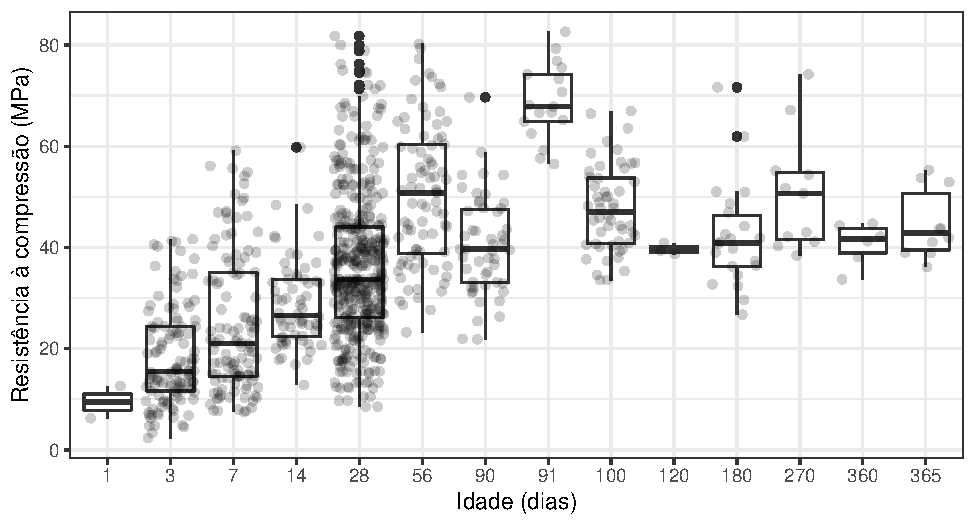
\includegraphics{paper_PT_files/figure-latex/boxplot-1} 

}

\caption{Boxplot - Resistência à compressão (MPa) vs idade (dias)}\label{fig:boxplot}
\end{figure}

Foi observado que as idades de 90, 91 e 100 dias provavelmente
representam extremos entre si das configurações de ingredientes, uma vez
que são idades relativamente próximas porém com valores muito
diferentes, especialmente para 90 e 91.

~

Essa hipótese foi verificada utilizando o método de análise de
componente principal, aplicado às amostras dessas 3 idades
(\ref{show-pca-90-91-100}). A fígura \ref{fig:pca-90-91-100} mostra como
as amostras se relacionam umas com as outras (quais são parecidas ou
diferentes) e revelou como cada variável contribui para a análise. As
duas primeiras dimensões representam 37\% e 24\% respectivamente da
variância.

~

\begin{figure}

{\centering 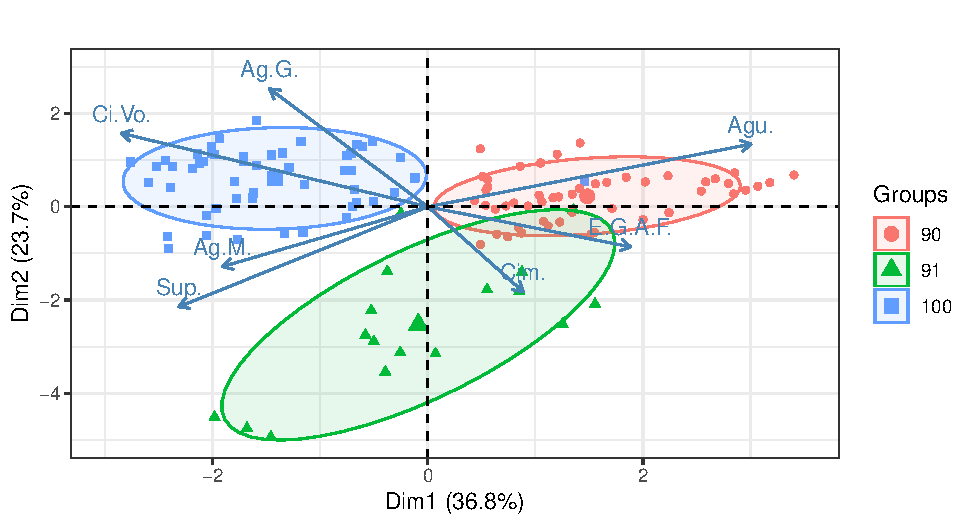
\includegraphics{paper_PT_files/figure-latex/pca-90-91-100-1} 

}

\caption{Análise componente principal - 90, 91 e 100 dias}\label{fig:pca-90-91-100}
\end{figure}

Outro ponto importante considerado, da própria natureza do concreto, é o
fato da taxa de crescimento de sua resistência à compressão diminuir com
o tempo, chegando a um certo valor de establidade. A figura
\ref{fig:mpa-on-time} mostra a resistência à compressão ao longo dos
dias para amostras com mais de 5 dados, ou seja, dados disponiveis para
no mínimo 6 idades distintas (\ref{show-mpa-on-time}).

~

\begin{figure}

{\centering 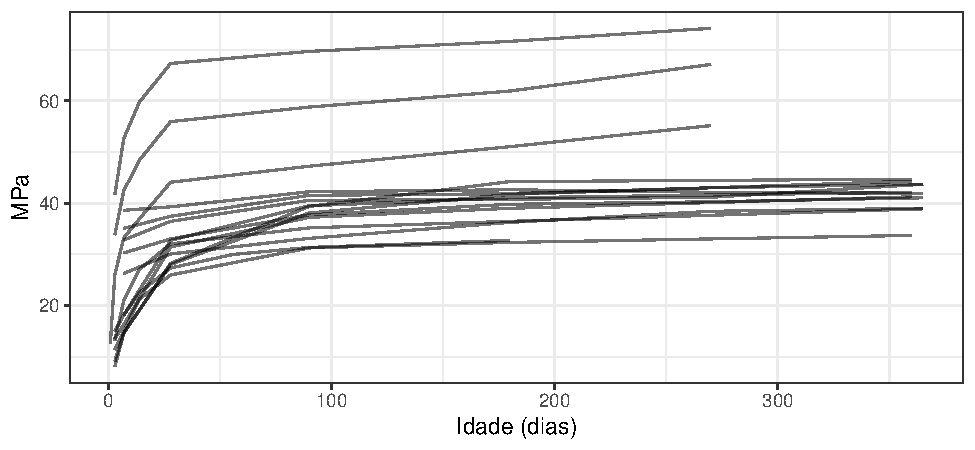
\includegraphics{paper_PT_files/figure-latex/mpa-on-time-1} 

}

\caption{Resistência à compressão ao longo do tempo}\label{fig:mpa-on-time}
\end{figure}

Pelos motivos apresentados nas figuras \ref{fig:boxplot},
\ref{fig:pca-90-91-100} e \ref{fig:mpa-on-time}, foi considerado que as
idades de 90, 91 e 100 dias podem ser agrupadas para melhorar a leitura
e diminuir o ruído das amostras. Elas foram convertidas para o mesmo
valor, que no caso foi escolhido a idade de 100 dias
(\ref{show-join-90-91-100}), pois como mostrado na figura
\ref{fig:mpa-on-time}, a resistência apenas aumenta, logo aos 100 dias a
resistência à compressão será maior ou igual ao valor de 90 ou 91 dias.

~

Mais um tópico analisado na seleção das idades foi a frequência
observada de cada valor de idade após essa transformação dos 90, 91 em
100 dias, mostrada na figura \ref{fig:freq-ages}. Alguns valores de dias
apresentam concentrações muito baixas de amostras, correndo o risco de
prejudicar mais do que ajudar na criação dos modelos, logo elas foram
removidas (\ref{show-remove-ages-lower-50}). O critério adotado foi
manter apenas idades com frequência maior que 50, ou seja, apenas os
valores de 3, 7, 14, 28, 56 e 100 dias.

~

\begin{figure}

{\centering 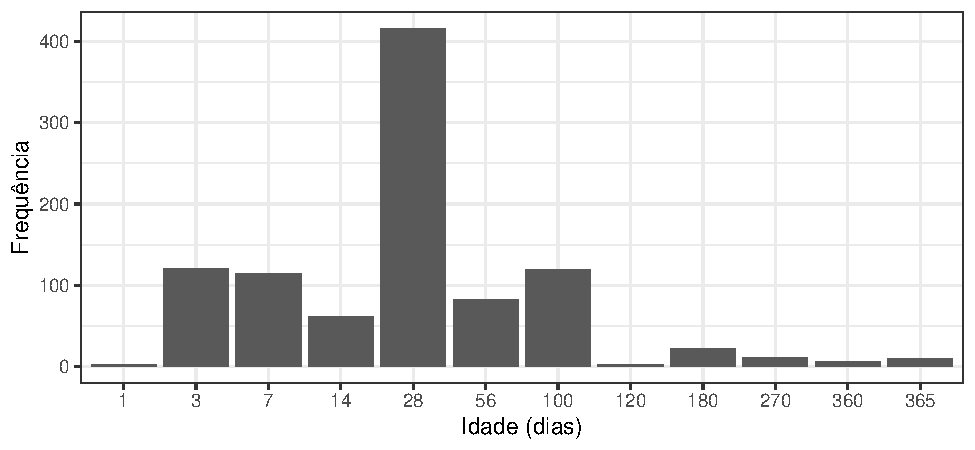
\includegraphics{paper_PT_files/figure-latex/freq-ages-1} 

}

\caption{Frequência das idades}\label{fig:freq-ages}
\end{figure}

\hypertarget{reorganizauxe7uxe3o-dos-dados}{%
\subsubsection{Reorganização dos
dados}\label{reorganizauxe7uxe3o-dos-dados}}

As amostras foram agrupadas para manter apenas uma amostra distinta de
cada conjunto de configuração das proporções dos ingredientes,
adicionando novas variáveis/colunas para a resistência em cada idade
(\ref{show-reorganizing-dat}). O resultado nas primeiras amostras após
esse processamento é mostrado na tabela \ref{tab:new-features}.

~

\begin{table}[H]

\caption{\label{tab:new-features}Primeiras 6 amostras reorganizadas}
\centering
\resizebox{\linewidth}{!}{
\begin{tabular}[t]{cccccccccccccc}
\toprule
\multicolumn{1}{c}{ID} & \multicolumn{1}{c}{Cimento} & \multicolumn{1}{c}{E.G.A.F.} & \multicolumn{1}{c}{C.Volante} & \multicolumn{1}{c}{Água} & \multicolumn{1}{c}{Superp.} & \multicolumn{1}{c}{A.Graúdo} & \multicolumn{1}{c}{A.Miúdo} & \multicolumn{1}{c}{3 dias} & \multicolumn{1}{c}{7 dias} & \multicolumn{1}{c}{14 dias} & \multicolumn{1}{c}{28 dias} & \multicolumn{1}{c}{56 dias} & \multicolumn{1}{c}{100 dias} \\
 & $kg/m^3$ & $kg/m^3$ & $kg/m^3$ & $kg/m^3$ & $kg/m^3$ & $kg/m^3$ & $kg/m^3$ & $MPa$ & $MPa$ & $MPa$ & $MPa$ & $MPa$ & $MPa$\\
\midrule
1 & 540.0 & 0.0 & 0 & 162 & 2.5 & 1040.0 & 676.0 &  &  &  & 79.99 &  & \\
\addlinespace
2 & 540.0 & 0.0 & 0 & 162 & 2.5 & 1055.0 & 676.0 &  &  &  & 61.89 &  & \\
\addlinespace
3 & 332.5 & 142.5 & 0 & 228 & 0.0 & 932.0 & 594.0 &  & 30.28 &  & 33.02 &  & 37.72\\
\addlinespace
5 & 198.6 & 132.4 & 0 & 192 & 0.0 & 978.4 & 825.5 & 9.13 & 14.64 &  & 28.02 &  & 38.07\\
\addlinespace
6 & 266.0 & 114.0 & 0 & 228 & 0.0 & 932.0 & 670.0 &  &  &  & 45.85 &  & 47.03\\
\addlinespace
7 & 380.0 & 95.0 & 0 & 228 & 0.0 & 932.0 & 594.0 &  & 32.82 &  & 36.45 &  & 40.56\\
\bottomrule
\end{tabular}}
\end{table}

O número de amostras e amostras distintas após toda essa manipulação
permaneceu o mesmo, um total de 416 (\ref{show-total-samples-2}).

\hypertarget{adicionando-novas-variuxe1veis}{%
\subsubsection{Adicionando novas
variáveis}\label{adicionando-novas-variuxe1veis}}

Para finalizar a preparação dos dados, novas colunas foram adicionadas
ao conjunto de amostras (\ref{show-new-features-2}). Iniciando pela
classe do concreto, por exemplo se a resistência à compressão está entre
25 e 30, recebe a classe \emph{C25}. A inclusão da classe foi importânte
pois a resistência em \(MPa\) é uma variável contínua, que será
utilizada nos modelos de regressão, mas a classe como variável discreta
pode fornecer outro ângulo de visualização dos dados. Também foi
adicionado o traço aproximado do concreto, que representa as proporções
de agregados (miúdo e graúdo) para o cimento. Outras proporções entre os
principais ingredientes também foram adicionadas. As novas variáveis são
apresentadas na tabela \ref{tab:new-features-table}.

\begin{table}[H]

\caption{\label{tab:new-features-table}Novas variáveis}
\centering
\resizebox{\linewidth}{!}{
\begin{tabular}[t]{c>{\centering\arraybackslash}p{1.5cm}>{\centering\arraybackslash}p{2cm}>{\centering\arraybackslash}p{1.7cm}>{\centering\arraybackslash}p{1.7cm}>{\centering\arraybackslash}p{1.7cm}>{\centering\arraybackslash}p{1.7cm}>{\centering\arraybackslash}p{1.7cm}>{\centering\arraybackslash}p{1.7cm}}
\toprule
ID & Classe & Traço aproximado & Água / Cimento & A.Miúdo / Cimento & A.Graúdo / Cimento & A.Miúdo / A.Graúdo & Água / A.Graúdo & Água / A.Miúdo\\
\midrule
1 & C75 & 1:1:2 & 0.3000 & 1.2519 & 1.9259 & 0.6500 & 0.1558 & 0.2396\\
\addlinespace
2 & C60 & 1:1:2 & 0.3000 & 1.2519 & 1.9537 & 0.6408 & 0.1536 & 0.2396\\
\addlinespace
3 & C30 & 1:2:3 & 0.6857 & 1.7865 & 2.8030 & 0.6373 & 0.2446 & 0.3838\\
\addlinespace
5 & C25 & 1:4:5 & 0.9668 & 4.1566 & 4.9265 & 0.8437 & 0.1962 & 0.2326\\
\addlinespace
6 & C45 & 1:3:4 & 0.8571 & 2.5188 & 3.5038 & 0.7189 & 0.2446 & 0.3403\\
\addlinespace
7 & C35 & 1:2:2 & 0.6000 & 1.5632 & 2.4526 & 0.6373 & 0.2446 & 0.3838\\
\bottomrule
\end{tabular}}
\end{table}

\hypertarget{visualizauxe7uxe3o-dos-dados}{%
\subsection{Visualização dos dados}\label{visualizauxe7uxe3o-dos-dados}}

Para avaliar a necessidade de mais manipulações antes da construção dos
modelos, nesta etapa as 416 amostras já processadas foram visualizadas e
analisadas.

\hypertarget{estatistica-descritiva}{%
\subsubsection{Estatistica descritiva}\label{estatistica-descritiva}}

A tabela \ref{tab:stat-summ} apresenta os dados estatísticos das
variáveis contínuas (\ref{show-stat-summ}). A linha de \emph{Null}
representa o número de valores zerados para os ingredientes, e a linha
\emph{NA} representa o número de dados faltando. Como as amostras foram
filtradas para manter apenas conjuntos de amostras com valores
conhecidos da resistência à compressão aos 28 dias, o número de
\emph{NAs} é zero para essa idade. A figura
\ref{fig:stat-summ-categorical} apresenta os dados estatísticos das
variáveis discretas (\ref{show-stat-summ-categorical}).

~

\begin{table}[H]

\caption{\label{tab:stat-summ}Estatística descritiva - variáveis contínuas}
\centering
\resizebox{\linewidth}{!}{
\begin{tabular}[t]{>{\raggedright\arraybackslash}p{1.5cm}cccccccc>{\centering\arraybackslash}p{1.5cm}>{\centering\arraybackslash}p{1.5cm}>{\centering\arraybackslash}p{1.5cm}>{\centering\arraybackslash}p{1.5cm}>{\centering\arraybackslash}p{1.5cm}>{\centering\arraybackslash}p{1.5cm}}
\toprule
  & Amostras & Null & NA & Min & Max & Intervalo & Soma & Mediana & Média & Erro padrão  da média & Intervalo de confiânça da média & Variância & Desvio Padrão & Coeficiênte de variação\\
\midrule
Cimento & 416 & 0 & 0 & 102.00 & 540.00 & 438.00 & 109373.10 & 257.70 & 262.92 & 5.10 & 10.02 & 10817.50 & 104.01 & 0.40\\
\addlinespace
E.G.A.F. & 416 & 174 & 0 & 0.00 & 359.40 & 359.40 & 35824.60 & 94.25 & 86.12 & 4.32 & 8.49 & 7755.00 & 88.06 & 1.02\\
\addlinespace
Cinza Volante & 416 & 202 & 0 & 0.00 & 200.10 & 200.10 & 26389.00 & 71.25 & 63.44 & 3.26 & 6.40 & 4407.81 & 66.39 & 1.05\\
\addlinespace
Água & 416 & 0 & 0 & 121.80 & 247.00 & 125.20 & 76335.60 & 185.00 & 183.50 & 0.94 & 1.86 & 370.73 & 19.25 & 0.10\\
\addlinespace
Superplast. & 416 & 107 & 0 & 0.00 & 32.20 & 32.20 & 2871.30 & 7.60 & 6.90 & 0.26 & 0.52 & 28.85 & 5.37 & 0.78\\
\addlinespace
A.Graúdo & 416 & 0 & 0 & 801.00 & 1145.00 & 344.00 & 397799.90 & 953.35 & 956.25 & 4.12 & 8.10 & 7063.06 & 84.04 & 0.09\\
\addlinespace
A.Miúdo & 416 & 0 & 0 & 594.00 & 992.60 & 398.60 & 317809.80 & 769.65 & 763.97 & 3.59 & 7.06 & 5371.89 & 73.29 & 0.10\\
\addlinespace
3 dias & 121 & 0 & 295 & 2.33 & 41.64 & 39.31 & 2210.82 & 15.52 & 18.27 & 0.87 & 1.72 & 91.64 & 9.57 & 0.52\\
\addlinespace
7 dias & 114 & 0 & 302 & 7.51 & 59.09 & 51.58 & 2845.52 & 21.06 & 24.96 & 1.29 & 2.55 & 188.81 & 13.74 & 0.55\\
\addlinespace
14 dias & 62 & 0 & 354 & 12.84 & 59.76 & 46.92 & 1782.56 & 26.54 & 28.75 & 1.10 & 2.19 & 74.62 & 8.64 & 0.30\\
\addlinespace
28 dias & 416 & 0 & 0 & 8.54 & 81.75 & 73.21 & 15101.13 & 33.72 & 36.30 & 0.70 & 1.38 & 206.30 & 14.36 & 0.40\\
\addlinespace
56 dias & 83 & 0 & 333 & 23.25 & 80.20 & 56.95 & 4178.77 & 50.77 & 50.35 & 1.52 & 3.02 & 190.82 & 13.81 & 0.27\\
\addlinespace
100 dias & 120 & 0 & 296 & 21.86 & 82.60 & 60.74 & 5701.90 & 45.61 & 47.52 & 1.17 & 2.31 & 163.40 & 12.78 & 0.27\\
\addlinespace
Água/ Cimento & 416 & 0 & 0 & 0.27 & 1.88 & 1.62 & 340.60 & 0.73 & 0.82 & 0.02 & 0.03 & 0.11 & 0.34 & 0.41\\
\addlinespace
A.Miúdo/ Cimento & 416 & 0 & 0 & 1.14 & 9.24 & 8.10 & 1415.82 & 2.94 & 3.40 & 0.07 & 0.14 & 1.96 & 1.40 & 0.41\\
\addlinespace
A.Graúdo/ Cimento & 416 & 0 & 0 & 1.55 & 8.70 & 7.14 & 1761.06 & 3.67 & 4.23 & 0.08 & 0.16 & 2.70 & 1.64 & 0.39\\
\addlinespace
A.Miúdo / A.Graúdo & 416 & 0 & 0 & 0.53 & 1.16 & 0.63 & 335.42 & 0.80 & 0.81 & 0.01 & 0.01 & 0.01 & 0.11 & 0.14\\
\addlinespace
Água / A.Graúdo & 416 & 0 & 0 & 0.12 & 0.29 & 0.17 & 80.66 & 0.19 & 0.19 & 0.00 & 0.00 & 0.00 & 0.03 & 0.16\\
\addlinespace
Água / A.Miúdo & 416 & 0 & 0 & 0.13 & 0.38 & 0.26 & 101.26 & 0.24 & 0.24 & 0.00 & 0.00 & 0.00 & 0.04 & 0.17\\
\bottomrule
\end{tabular}}
\end{table}
\begin{figure}

{\centering 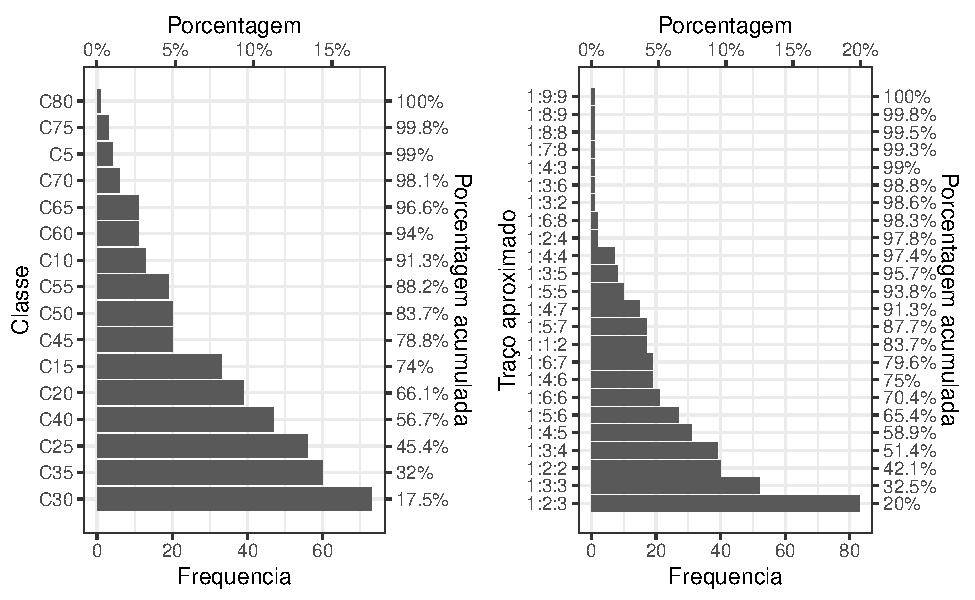
\includegraphics{paper_PT_files/figure-latex/stat-summ-categorical-1} 

}

\caption{Estatística descritiva - variáveis discretas}\label{fig:stat-summ-categorical}
\end{figure}

\hypertarget{correlauxe7uxe3o-dos-ingredientes-e-resistuxeancia-uxe0-compressuxe3o}{%
\subsubsection{Correlação dos ingredientes e resistência à
compressão}\label{correlauxe7uxe3o-dos-ingredientes-e-resistuxeancia-uxe0-compressuxe3o}}

A figura \ref{fig:correlation} apresenta a correlação das variáveis para
cada conjunto de idades (\ref{show-correlation}). A figura
\ref{fig:correlation-mpa} apresenta os mesmos dados, mas em vez de
correlacionar todos, correlaciona apenas com a resistência à compressão,
mostrando os valores mais detalhadamente (\ref{show-correlation-mpa}).

~

\begin{figure}

{\centering 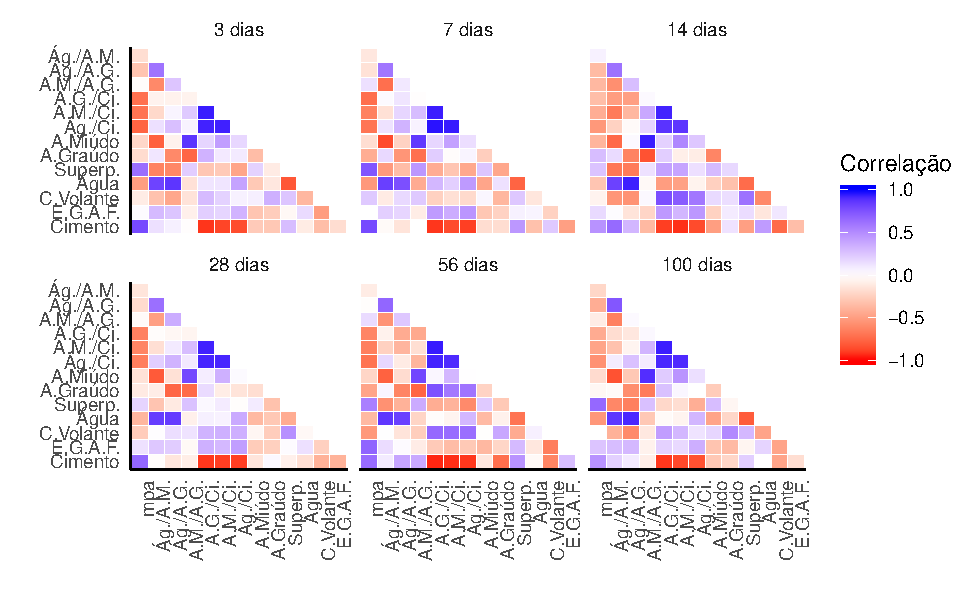
\includegraphics{paper_PT_files/figure-latex/correlation-1} 

}

\caption{Correlações em cada idade}\label{fig:correlation}
\end{figure}
\begin{figure}

{\centering 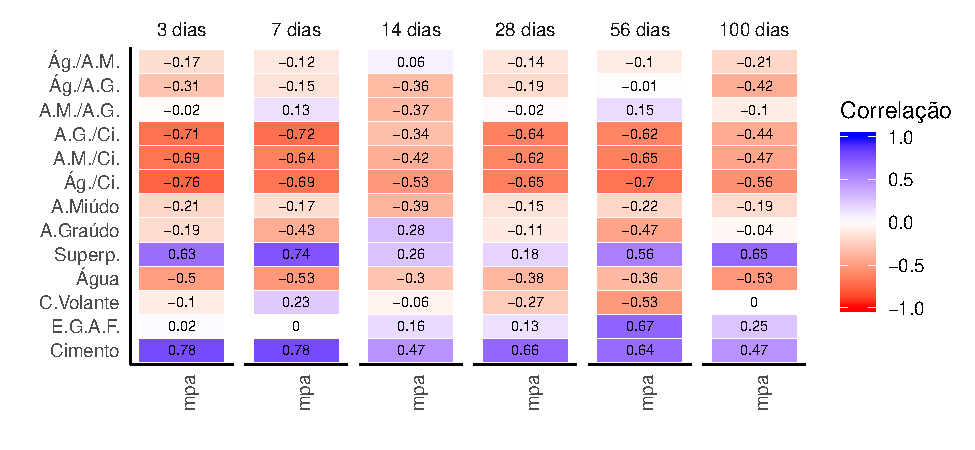
\includegraphics{paper_PT_files/figure-latex/correlation-mpa-1} 

}

\caption{Correlação das variáveis com a resistência à compressão no tempo}\label{fig:correlation-mpa}
\end{figure}

A interpretação da figura \ref{fig:correlation-mpa} sugere que a
resistência do concreto está relacionada positivamente principalmente
com os ingredientes cimento e superplastificante e negativamente com a
água e agregado miúdo. Quanto menor a quantidade de cimento para os
agregados e para água, mais negativamente estão correlacionados com a
resistência à compressão.

~

\begin{figure}

{\centering 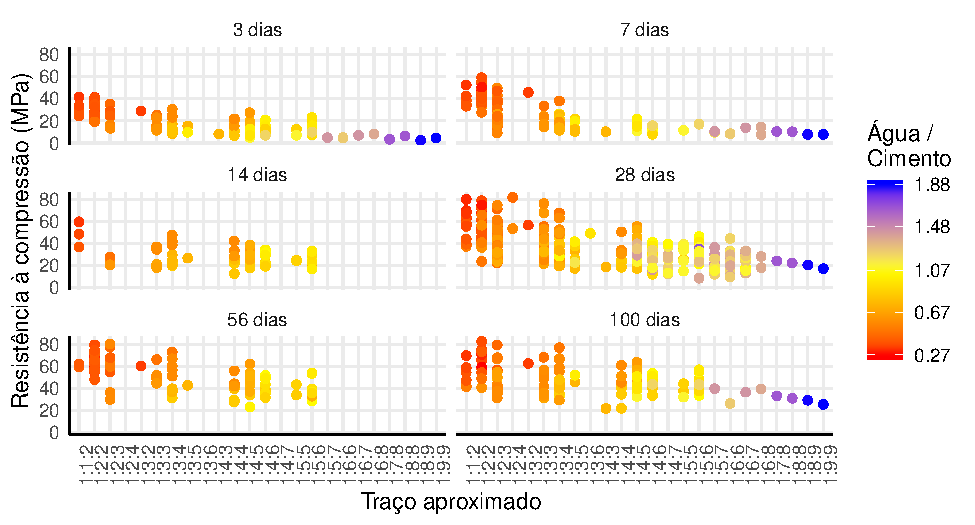
\includegraphics{paper_PT_files/figure-latex/mix-app-mpa-1} 

}

\caption{Relação entre o traço aproximado, água, resistência à compressão e idade}\label{fig:mix-app-mpa}
\end{figure}
\begin{figure}

{\centering 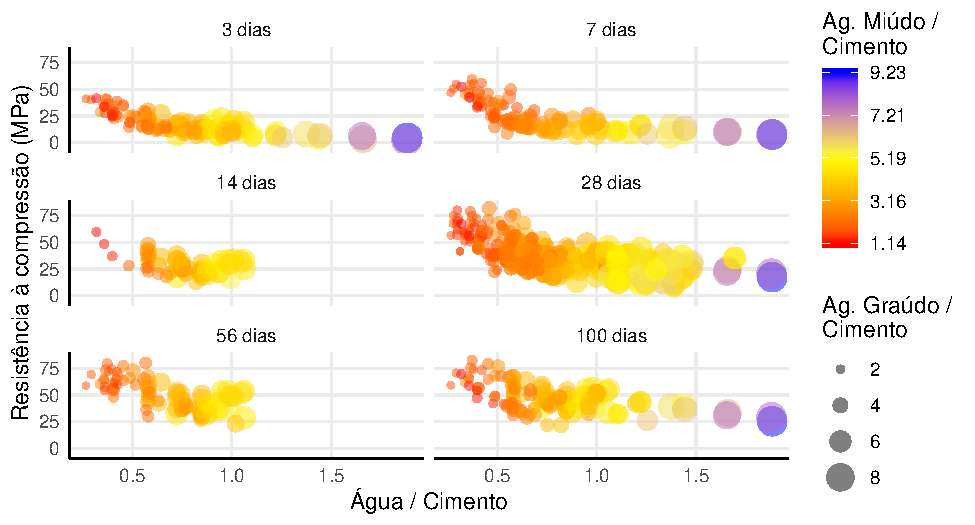
\includegraphics{paper_PT_files/figure-latex/mix-mpa-1} 

}

\caption{Relação das principais proporções do concreto}\label{fig:mix-mpa}
\end{figure}

As figuras \ref{fig:mix-app-mpa} e \ref{fig:mix-mpa} mostram a relação
entre os principais ingredientes (conhecida como traço) em relação à
resistência à compressão (\ref{show-mix-app-mpa} e \ref{show-mix-mpa}).
A interpretação dessas figuras mostra que quanto maior a quantidade de
cimento em relação aos outros ingredientes, maior será a resistência à
compressão.

\hypertarget{distribuiuxe7uxe3o-das-variuxe1veis}{%
\subsubsection{Distribuição das
variáveis}\label{distribuiuxe7uxe3o-das-variuxe1veis}}

A figura \ref{fig:vars-distribution} mostra a distribuição das variáveis
nas amostras (\ref{show-vars-distribution}). Foi calculado utilizando
apenas os dados aos 28 dias.

~

\begin{figure}

{\centering 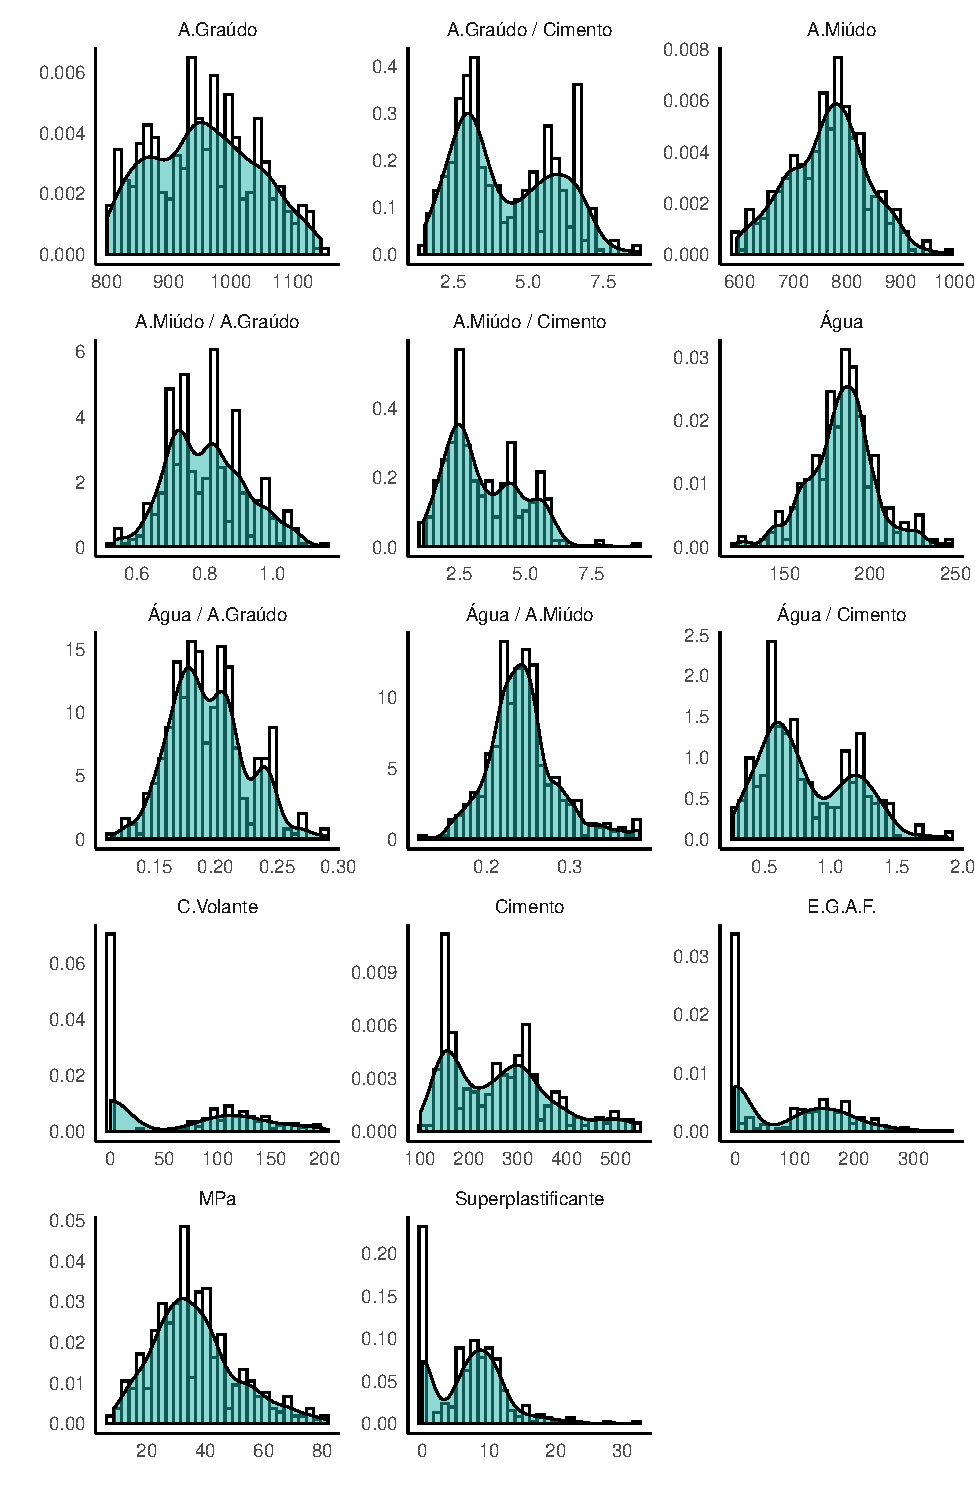
\includegraphics{paper_PT_files/figure-latex/vars-distribution-1} 

}

\caption{Distribuição das variáveis}\label{fig:vars-distribution}
\end{figure}

De outra forma, a figura \ref{fig:vars-distribution-time} mostra a
distribuição dos ingredientes e da resistência à compressão para cada
conjunto de idades (\ref{show-vars-distribution-time}), ou seja, no caso
dos 28 dias apresenta a mesma informação que a figura
\ref{fig:vars-distribution}. Através dela é visualizado que como
esperado, a resistência à compressão gradualmente aumenta ao longo do
tempo. Além disso é visualizado que a concentração dos ingredientes
podem variar muito quando estratíficado pelas idades.

\begin{figure}

{\centering 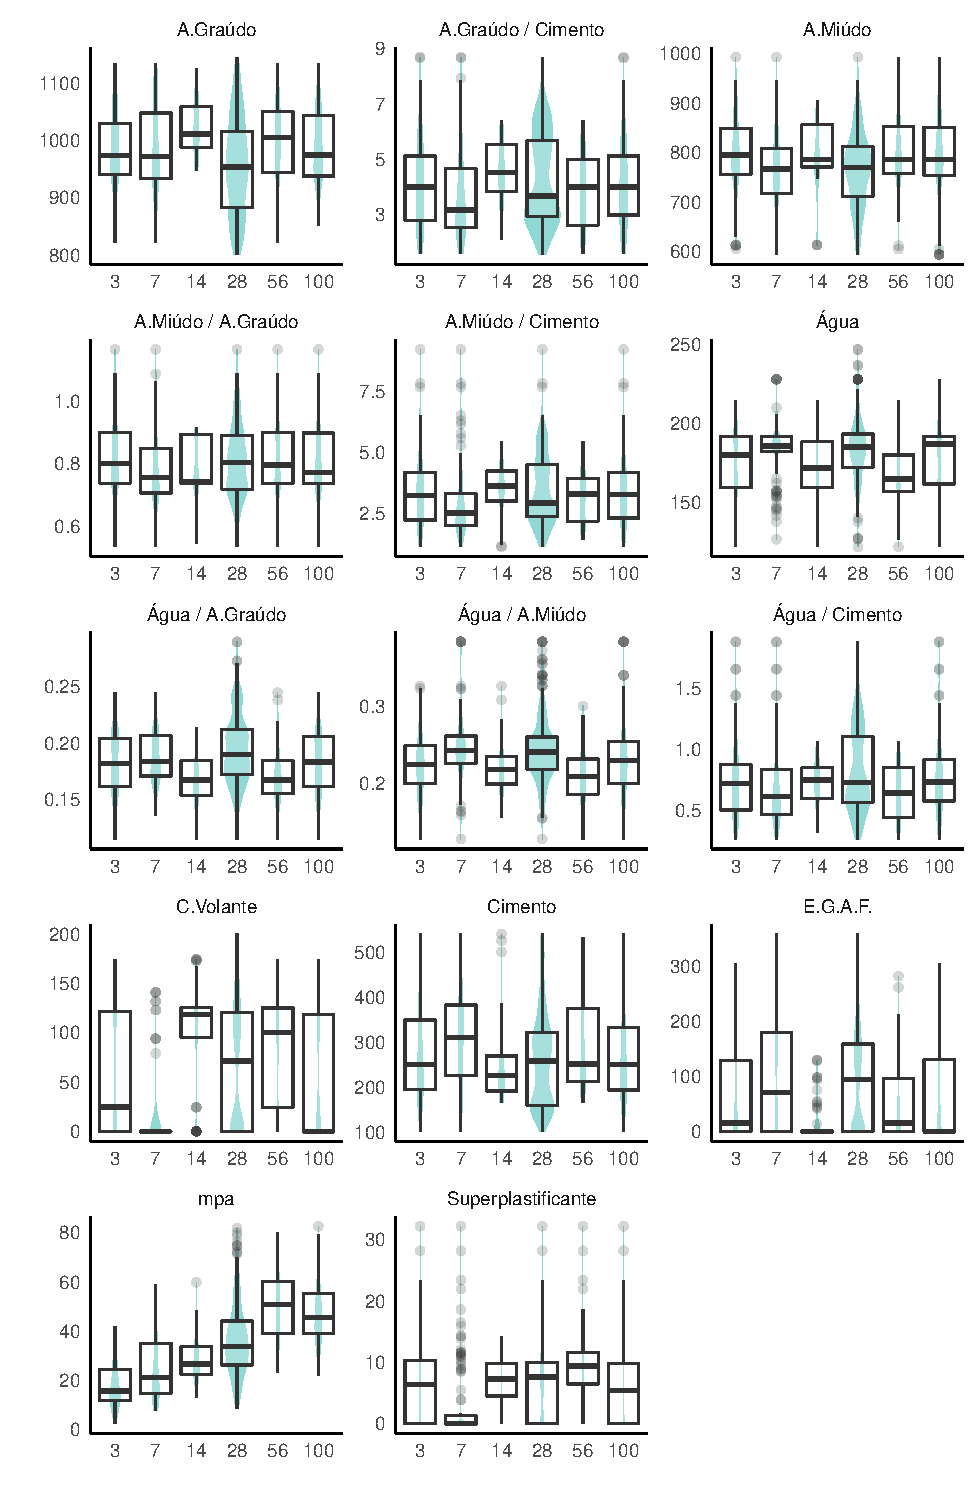
\includegraphics{paper_PT_files/figure-latex/vars-distribution-time-1} 

}

\caption{Distribuição das variáveis em relação a idade}\label{fig:vars-distribution-time}
\end{figure}

\hypertarget{anuxe1lise-de-componente-principal}{%
\subsubsection{Análise de componente
principal}\label{anuxe1lise-de-componente-principal}}

Na figura \ref{fig:pca}, utilizando uma classificação alternativa, foi
realizada a análise de componente principal nos ingredientes das
amostras (\ref{show-pca}). A classificação separa o concreto em 4 grupos
de resistência a compressão diferentes, baixo até \emph{20 MPa}, normal
até \emph{40 MPa}, médio até \emph{70 MPa} e alto acima disso. É
possivel perceber que os grupos se sobrepõem, mas existem uma
diferenciação entre o grupo alto e baixo.

\begin{figure}

{\centering 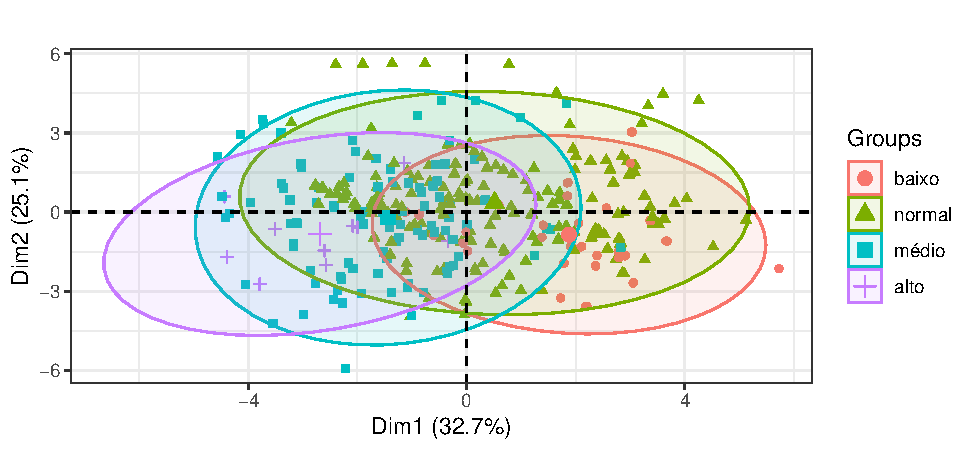
\includegraphics{paper_PT_files/figure-latex/pca-1} 

}

\caption{Análise componente principal nos ingredientes}\label{fig:pca}
\end{figure}

\hypertarget{modelos-de-machine-learning}{%
\subsection{Modelos de machine
learning}\label{modelos-de-machine-learning}}

O desenvolvimento dos modelos de machine learning foi realizado com o
pacote \emph{caret} (Kuhn 2020) e baseado em Irizarry (2019) e Kuhn
(2008).

\hypertarget{pre-processamento-e-separauxe7uxe3o-dos-dados}{%
\subsubsection{Pre processamento e separação dos
dados}\label{pre-processamento-e-separauxe7uxe3o-dos-dados}}

Como existe a variável categórica para o traço aproximado do concreto,
foi realizada a conversão dessa variável em variáveis fictiícias
(\emph{dummy vars}) (\ref{show-dummy-var}), passando de 22 colunas (id,
classe, resistência à compressão e mais 19 \emph{features}) para 45
colunas, uma adição de 23 variáveis, uma para cada traço aproximado.

~

As amostras foram separadas baseado nas idades. Foram criados um
conjunto de dados para cada valor de idade, totalizando 6 conjuntos
diferentes (\ref{show-preparation}). Para fins ilustrativos, as
primeiras 18 de 45 colunas das primeiras 6 amostras do conjunto de 28
dias são mostradas na tabela \ref{tab:table-preparated-samples}.

~

\begin{table}[H]

\caption{\label{tab:table-preparated-samples}Primeiras 18 colunas das primeiras 6 amostras de 28 dias}
\centering
\resizebox{\linewidth}{!}{
\begin{tabular}[t]{cccccccccccccccccc}
\toprule
\multicolumn{1}{c}{ID} & \multicolumn{1}{c}{Cimento} & \multicolumn{1}{c}{E.G.A.F.} & \multicolumn{1}{c}{C.Vol.} & \multicolumn{1}{c}{Água} & \multicolumn{1}{c}{Superp.} & \multicolumn{1}{c}{A.Graúdo} & \multicolumn{1}{c}{A.Miúdo} & \multicolumn{1}{c}{MPa} & \multicolumn{1}{c}{Classe} & \multicolumn{1}{c}{Ág./} & \multicolumn{1}{c}{A.M./} & \multicolumn{1}{c}{A.G./} & \multicolumn{1}{c}{A.M./} & \multicolumn{1}{c}{Ág./} & \multicolumn{1}{c}{Ág./} & \multicolumn{2}{c}{Traço Apox.} \\
 & $kg/m^3$ & $kg/m^3$ & $kg/m^3$ & $kg/m^3$ & $kg/m^3$ & $kg/m^3$ & $kg/m^3$ & $MPa$ &  & Ci. & Ci. & Ci. & A.G. & A.G. & Ag.M. & 1:1:2 & 1:2:2\\
\midrule
1 & 540.0 & 0.0 & 0 & 162 & 2.5 & 1040.0 & 676.0 & 79.99 & C75 & 0.30 & 1.25 & 1.93 & 0.65 & 0.16 & 0.24 & 1 & 0\\
\addlinespace
2 & 540.0 & 0.0 & 0 & 162 & 2.5 & 1055.0 & 676.0 & 61.89 & C60 & 0.30 & 1.25 & 1.95 & 0.64 & 0.15 & 0.24 & 1 & 0\\
\addlinespace
3 & 332.5 & 142.5 & 0 & 228 & 0.0 & 932.0 & 594.0 & 33.02 & C30 & 0.69 & 1.79 & 2.80 & 0.64 & 0.24 & 0.38 & 0 & 0\\
\addlinespace
5 & 198.6 & 132.4 & 0 & 192 & 0.0 & 978.4 & 825.5 & 28.02 & C25 & 0.97 & 4.16 & 4.93 & 0.84 & 0.20 & 0.23 & 0 & 0\\
\addlinespace
6 & 266.0 & 114.0 & 0 & 228 & 0.0 & 932.0 & 670.0 & 45.85 & C45 & 0.86 & 2.52 & 3.50 & 0.72 & 0.24 & 0.34 & 0 & 0\\
\addlinespace
7 & 380.0 & 95.0 & 0 & 228 & 0.0 & 932.0 & 594.0 & 36.45 & C35 & 0.60 & 1.56 & 2.45 & 0.64 & 0.24 & 0.38 & 0 & 1\\
\bottomrule
\end{tabular}}
\end{table}

Para cada um dos 6 conjuntos foi verificado a existência ou não de
variáveis com variância próxima a zero e sua subsequênte remoção
(\ref{show-nzv}). Muitas das 23 variáveis adicionadas referentes ao
traço aproximado do concreto foram removidas devido a esse fato. Além
delas, no caso do conjunto de 7 dias, a variável cinza volante também
foi removida. Depois foi verificado que não existem variáveis com alta
correlação, acima de 0,999 em nenhum dos 6 conjuntos de dados
(\ref{show-cors}). Após essas etapas, os conjuntos de amostras
apresentaram 24, 21, 23, 23, 24 e 25 colunas respectivamente para as
idades em sequência crescente.

~

A etapa de centralização e normalização das variáveis foi realizada mais
a frente, junto com a aplicação dos modelos, pois é mais simples fazer
dessa forma com o pacote \emph{caret}. Se fosse realizada nesse momento,
seria nescessário manualmente desfazer essas transformações nas
previsões. O \emph{caret} permite transformar antes do treino dos
modelos e já transforma de volta os resultados.

~

Cada um dos conjuntos de dados foi separado em conjuntos de teste e
treino, \emph{20\%} e \emph{80\%} respectivamente (\ref{show-split}). A
figura \ref{fig:dist-split} mostra como ficou a distribuição dos dados
entre os conjuntos em relação a resistência à compressão para cada
modelo (\ref{show-dist-split}).

\begin{figure}

{\centering 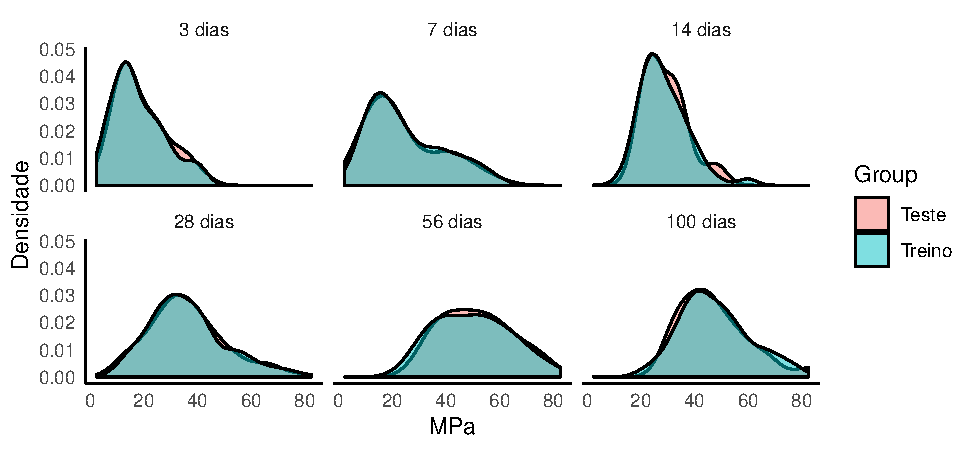
\includegraphics{paper_PT_files/figure-latex/dist-split-1} 

}

\caption{Distribuição dos conjuntos de teste e treino}\label{fig:dist-split}
\end{figure}

\hypertarget{medidas-de-performance}{%
\subsubsection{Medidas de performance}\label{medidas-de-performance}}

A avaliação da performance dos modelos foi realizada pela Raiz do Erro
Quadrático Médio (\emph{RMSE}). O \emph{RMSE} é a medida utilizada em
todos os trabalhos citados na introdução e permitirá a comparação dos
modelos na discussão.

\hypertarget{modelos-inguxeanuos}{%
\subsubsection{Modelos ingênuos}\label{modelos-inguxeanuos}}

Antes de criar os modelos verdadeiros, para fins de comparação, foram
criados modelos ingênuos. Eles simplesmente prevêem que a resistência à
compressão do conjunto de teste, é a média da resistência à compressão
do conjunto de treino (\ref{show-naive-model-reg}). Em outras palavras,
os modelos ingênuos são simplesmente o melhor palpite possível. Os
resultados podem ser conferidos na tabela
\ref{tab:table-naive-model-reg}.

\begin{table}[H]

\caption{\label{tab:table-naive-model-reg}Modelos ingênuos}
\centering
\begin{tabular}[t]{cccc}
\toprule
Idade & Média $MPa$ (treino) & RMSE (treino) & RMSE (teste)\\
\midrule
3 & 18.08887 & 9.591344 & 9.303229\\
\addlinespace
7 & 25.12383 & 13.731569 & 13.443646\\
\addlinespace
14 & 28.63980 & 8.786823 & 7.593319\\
\addlinespace
28 & 36.33605 & 14.361021 & 14.283824\\
\addlinespace
56 & 50.06555 & 13.968077 & 12.702112\\
\addlinespace
100 & 47.57000 & 12.758042 & 12.614652\\
\bottomrule
\end{tabular}
\end{table}

\hypertarget{escolha-do-algoruxedtimo}{%
\subsubsection{Escolha do algorítimo}\label{escolha-do-algoruxedtimo}}

O pacote \emph{caret} (Kuhn 2020) expõe mais de 200 algorítimos
diferentes para criar modelos de \emph{machine learning}. A documentação
do pacote apresenta um código inicial (``Models Clustered by Tag
Similarity'' 2020) como sugestão para selecionar um portifólio de
algóritmos mais distintos possíveis em relação à algum algorítimo
pré-selecionado, mas para agilidade e devido a limitações técnicas, foi
escolhido utilizar um algorítimo com a maior probabilidade de atingir o
melhor resultado possível. Segundo Fernandez-Delgado et al. (2014), que
comparou 179 algorítimos em 121 banco de dados diferentes, o algorítimo
mais provável de atingir os melhores resultados possíveis é o
\emph{Parallel Random Forest} (denominado \emph{prRF} no \emph{caret}).

\hypertarget{modelos-de-regressuxe3o}{%
\subsubsection{Modelos de regressão}\label{modelos-de-regressuxe3o}}

Como ao longo do processamento foram adicionadas novas variáveis (as
relações entre os ingredientes e mais algumas \emph{dummy vars} para
cada conjunto de idade), foram estudadas 5 possibilidades de
configurações das \emph{features} para os modelos:

~

\begin{enumerate}
\def\labelenumi{\arabic{enumi}.}
\tightlist
\item
  Todas as \emph{features};
\item
  Sem as \emph{dummy vars};
\item
  Apenas \emph{features} originais;
\item
  Apenas \emph{features} adicionadas;
\item
  Apenas \emph{features} adicionadas, sem as \emph{dummy vars};
\end{enumerate}

~

Construindo um modelo para cada uma dessas configurações utilizando o
conjunto de amostras aos 28 dias (\ref{show-test-models-reg}), mostrou
que a melhor opção é a configuração 2, ou seja, as \emph{dummy vars}
foram completamente descartadas, porém foram mantidas as outras novas
varáveis. Para fins ilustrativos, a tabela
\ref{tab:table-done-samples-28} mostra as primeiras 6 amostras do
conjunto de treino do modelo de 28 dias. As amostras dos outros modelos,
dos conjuntos de teste e treino são similares, sendo a única diferença
no modelo de 7 dias, que exlcui a cinza volante devido a variância
próxima a zero, realizado anteriormente.

\begin{table}[H]

\caption{\label{tab:table-done-samples-28}Primeiras 6 amostras do conjunto de treino do modelo de 28 dias}
\centering
\resizebox{\linewidth}{!}{
\begin{tabular}[t]{cccccccccccccc}
\toprule
\multicolumn{13}{c}{Features} & \multicolumn{1}{c}{Outcome} \\
\cmidrule(l{3pt}r{3pt}){1-13} \cmidrule(l{3pt}r{3pt}){14-14}
\multicolumn{1}{c}{Cimento} & \multicolumn{1}{c}{E.G.A.F.} & \multicolumn{1}{c}{C.Vol.} & \multicolumn{1}{c}{Água} & \multicolumn{1}{c}{Superp.} & \multicolumn{1}{c}{A.Graúdo} & \multicolumn{1}{c}{A.Miúdo} & \multicolumn{1}{c}{Ág./} & \multicolumn{1}{c}{A.M./} & \multicolumn{1}{c}{A.G./} & \multicolumn{1}{c}{A.M./} & \multicolumn{1}{c}{Ág./} & \multicolumn{1}{c}{Ág./} & \multicolumn{1}{c}{y} \\
$kg/m^3$ & $kg/m^3$ & $kg/m^3$ & $kg/m^3$ & $kg/m^3$ & $kg/m^3$ & $kg/m^3$ & Ci. & Ci. & Ci. & A.G. & A.G. & Ag.M. & $MPa$\\
\midrule
540.0 & 0.0 & 0 & 162 & 2.5 & 1040.0 & 676.0 & 0.30 & 1.25 & 1.93 & 0.65 & 0.16 & 0.24 & 79.99\\
\addlinespace
540.0 & 0.0 & 0 & 162 & 2.5 & 1055.0 & 676.0 & 0.30 & 1.25 & 1.95 & 0.64 & 0.15 & 0.24 & 61.89\\
\addlinespace
266.0 & 114.0 & 0 & 228 & 0.0 & 932.0 & 670.0 & 0.86 & 2.52 & 3.50 & 0.72 & 0.24 & 0.34 & 45.85\\
\addlinespace
380.0 & 95.0 & 0 & 228 & 0.0 & 932.0 & 594.0 & 0.60 & 1.56 & 2.45 & 0.64 & 0.24 & 0.38 & 36.45\\
\addlinespace
475.0 & 0.0 & 0 & 228 & 0.0 & 932.0 & 594.0 & 0.48 & 1.25 & 1.96 & 0.64 & 0.24 & 0.38 & 39.29\\
\addlinespace
198.6 & 132.4 & 0 & 192 & 0.0 & 978.4 & 825.5 & 0.97 & 4.16 & 4.93 & 0.84 & 0.20 & 0.23 & 28.02\\
\bottomrule
\end{tabular}}
\end{table}

Para cada conjunto de idade foi criado um modelo utilizando o algorítimo
\emph{Parallel Random Forest}, definido anteriormente
(\ref{show-reg-models}). Para cada um dos 6 modelos, o parâmetro
\emph{mtry} foi otimizado, e foi realizado \emph{repeated
cross-validation}, dividindo em 10 ou 30 partes e repetindo 10 vezes.

\hypertarget{r-param-optimization-plots-echof-warningf-messagef-includef-ggplotfit_3-xlabcaracteruxedsticas-ylabrmse-ggplotfit_7-xlabcaracteruxedsticas-ylabrmse-ggplotfit_14-xlabcaracteruxedsticas-ylabrmse-ggplotfit_28-xlabcaracteruxedsticas-ylabrmse-ggplotfit_56-xlabcaracteruxedsticas-ylabrmse-ggplotfit_100-xlabcaracteruxedsticas-ylabrmse}{%
\section{\texorpdfstring{\texttt{\{r\ param-optimization-plots,\ echo=F,\ warning=F,\ message=F,\ include=F\}\ \#\ \ \#\ ggplot(fit\_3)\ +\ xlab("Características")\ +\ ylab("RMSE")\ \#\ ggplot(fit\_7)\ +\ xlab("Características")\ +\ ylab("RMSE")\ \#\ ggplot(fit\_14)\ +\ xlab("Características")\ +\ ylab("RMSE")\ \#\ ggplot(fit\_28)\ +\ xlab("Características")\ +\ ylab("RMSE")\ \#\ ggplot(fit\_56)\ +\ xlab("Características")\ +\ ylab("RMSE")\ \#\ ggplot(fit\_100)\ +\ xlab("Características")\ +\ ylab("RMSE")\ \#}}{\{r param-optimization-plots, echo=F, warning=F, message=F, include=F\} \#  \# ggplot(fit\_3) + xlab("Características") + ylab("RMSE") \# ggplot(fit\_7) + xlab("Características") + ylab("RMSE") \# ggplot(fit\_14) + xlab("Características") + ylab("RMSE") \# ggplot(fit\_28) + xlab("Características") + ylab("RMSE") \# ggplot(fit\_56) + xlab("Características") + ylab("RMSE") \# ggplot(fit\_100) + xlab("Características") + ylab("RMSE") \#}}\label{r-param-optimization-plots-echof-warningf-messagef-includef-ggplotfit_3-xlabcaracteruxedsticas-ylabrmse-ggplotfit_7-xlabcaracteruxedsticas-ylabrmse-ggplotfit_14-xlabcaracteruxedsticas-ylabrmse-ggplotfit_28-xlabcaracteruxedsticas-ylabrmse-ggplotfit_56-xlabcaracteruxedsticas-ylabrmse-ggplotfit_100-xlabcaracteruxedsticas-ylabrmse}}

\hypertarget{resultados}{%
\section{Resultados}\label{resultados}}

O \emph{RMSE} de teste de cada modelo em ordem crescente de idade foi
respectivamente 3.31, 4.36, 4.62, 4.72, 5.94 e 5.85. A tabela
\ref{tab:table-reg-models} apresenta os detalhes e resultados de cada
modelo (\ref{show-table-reg-models}). A figura
\ref{fig:results-comparison} compara os valores reais e previstos
(\ref{show-results-comparison}), e as tabelas seguintes mostram os
melhores e piores resultados de cada modelo (\ref{show-table-10}).

\begin{table}[H]

\caption{\label{tab:table-reg-models}Resultados dos modelos de regressão}
\centering
\begin{tabular}[t]{cccccc}
\toprule
Modelo & mtry & CV & Repetições & RMSE (treino) & RMSE (teste)\\
\midrule
3 dias & 6 & 30 & 10 & 3.905196 & 3.310370\\
\addlinespace
7 dias & 2 & 10 & 10 & 4.475981 & 4.361987\\
\addlinespace
14 dias & 13 & 30 & 10 & 5.136687 & 4.620515\\
\addlinespace
28 dias & 11 & 30 & 10 & 5.847334 & 4.716698\\
\addlinespace
56 dias & 8 & 30 & 10 & 6.702565 & 5.939163\\
\addlinespace
100 dias & 8 & 10 & 10 & 6.381940 & 5.851088\\
\bottomrule
\end{tabular}
\end{table}
\begin{figure}

{\centering 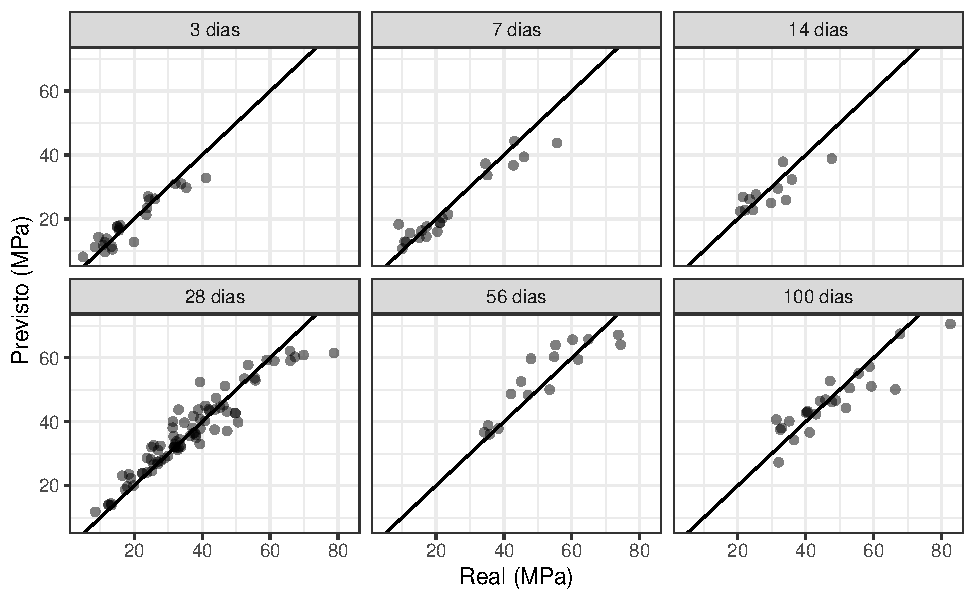
\includegraphics{paper_PT_files/figure-latex/results-comparison-1} 

}

\caption{Comparação dos valores reais e previstos em cada modelo}\label{fig:results-comparison}
\end{figure}
\begin{table}[H]

\caption{\label{tab:table-10}Modelo de 3 dias}
\centering
\begin{tabular}[t]{ccc>{\centering\arraybackslash}p{1cm}ccc}
\toprule
\multicolumn{3}{c}{10 melhores} & \multicolumn{1}{c}{} & \multicolumn{3}{c}{10 piores} \\
\cmidrule(l{3pt}r{3pt}){1-3} \cmidrule(l{3pt}r{3pt}){5-7}
Real & Previsto & Erro &  & Real & Previsto & Erro\\
\midrule
26.06 & 26.297746 & 0.2377457 &  & 41.10 & 32.758262 & -8.341738\\
\addlinespace
23.80 & 23.432367 & -0.3676333 &  & 19.93 & 12.732172 & -7.197828\\
\addlinespace
15.52 & 16.436292 & 0.9162920 &  & 35.30 & 29.781989 & -5.518011\\
\addlinespace
10.76 & 11.830651 & 1.0706507 &  & 9.45 & 14.316742 & 4.866742\\
\addlinespace
32.11 & 30.977619 & -1.1323807 &  & 4.90 & 8.154245 & 3.254245\\
\addlinespace
11.36 & 12.660044 & 1.3000440 &  & 13.57 & 10.464572 & -3.105428\\
\addlinespace
15.62 & 17.079698 & 1.4596980 &  & 24.10 & 27.016321 & 2.916321\\
\addlinespace
24.39 & 26.018261 & 1.6282610 &  & 33.80 & 31.045796 & -2.754204\\
\addlinespace
11.41 & 9.688879 & -1.7211213 &  & 8.49 & 11.196910 & 2.706910\\
\addlinespace
11.85 & 13.788864 & 1.9388640 &  & 14.99 & 17.677379 & 2.687379\\
\bottomrule
\end{tabular}
\end{table}

\begin{table}[H]

\caption{\label{tab:table-10}Modelo de 7 dias}
\centering
\begin{tabular}[t]{ccc>{\centering\arraybackslash}p{1cm}ccc}
\toprule
\multicolumn{3}{c}{10 melhores} & \multicolumn{1}{c}{} & \multicolumn{3}{c}{10 piores} \\
\cmidrule(l{3pt}r{3pt}){1-3} \cmidrule(l{3pt}r{3pt}){5-7}
Real & Previsto & Erro &  & Real & Previsto & Erro\\
\midrule
17.24 & 17.61947 & 0.3794733 &  & 55.60 & 43.71082 & -11.889177\\
\addlinespace
15.75 & 16.29318 & 0.5431847 &  & 9.01 & 18.32999 & 9.319987\\
\addlinespace
10.09 & 10.67438 & 0.5843837 &  & 45.90 & 39.45277 & -6.447230\\
\addlinespace
15.07 & 14.10010 & -0.9698955 &  & 42.80 & 36.78526 & -6.014737\\
\addlinespace
43.11 & 44.35190 & 1.2419040 &  & 20.42 & 16.03647 & -4.383533\\
\addlinespace
35.10 & 33.69951 & -1.4004926 &  & 12.37 & 15.58829 & 3.218292\\
\addlinespace
11.17 & 12.71080 & 1.5408013 &  & 17.17 & 14.38220 & -2.787795\\
\addlinespace
21.86 & 20.23260 & -1.6274033 &  & 34.57 & 37.26745 & 2.697450\\
\addlinespace
10.79 & 12.85092 & 2.0609233 &  & 21.16 & 18.79017 & -2.369827\\
\addlinespace
23.52 & 21.42631 & -2.0936880 &  & 21.18 & 18.84231 & -2.337694\\
\bottomrule
\end{tabular}
\end{table}

\begin{table}[H]

\caption{\label{tab:table-10}Modelo de 14 dias}
\centering
\begin{tabular}[t]{ccc>{\centering\arraybackslash}p{1cm}ccc}
\toprule
\multicolumn{3}{c}{10 melhores} & \multicolumn{1}{c}{} & \multicolumn{3}{c}{10 piores} \\
\cmidrule(l{3pt}r{3pt}){1-3} \cmidrule(l{3pt}r{3pt}){5-7}
Real & Previsto & Erro &  & Real & Previsto & Erro\\
\midrule
22.14 & 22.69248 & 0.5524823 &  & 47.71 & 38.87416 & -8.835845\\
\addlinespace
20.77 & 22.36561 & 1.5956093 &  & 34.24 & 25.88502 & -8.354984\\
\addlinespace
24.45 & 22.74412 & -1.7058757 &  & 21.50 & 26.91740 & 5.417403\\
\addlinespace
25.37 & 27.62261 & 2.2526130 &  & 29.75 & 25.02926 & -4.720744\\
\addlinespace
31.81 & 29.53499 & -2.2750130 &  & 33.36 & 37.88168 & 4.521675\\
\addlinespace
23.51 & 26.19615 & 2.6861493 &  & 35.96 & 32.35358 & -3.606417\\
\addlinespace
35.96 & 32.35358 & -3.6064167 &  & 23.51 & 26.19615 & 2.686149\\
\addlinespace
33.36 & 37.88168 & 4.5216750 &  & 31.81 & 29.53499 & -2.275013\\
\addlinespace
29.75 & 25.02926 & -4.7207443 &  & 25.37 & 27.62261 & 2.252613\\
\addlinespace
21.50 & 26.91740 & 5.4174030 &  & 24.45 & 22.74412 & -1.705876\\
\bottomrule
\end{tabular}
\end{table}

\begin{table}[H]

\caption{\label{tab:table-10}Modelo de 28 dias}
\centering
\begin{tabular}[t]{ccc>{\centering\arraybackslash}p{1cm}ccc}
\toprule
\multicolumn{3}{c}{10 melhores} & \multicolumn{1}{c}{} & \multicolumn{3}{c}{10 piores} \\
\cmidrule(l{3pt}r{3pt}){1-3} \cmidrule(l{3pt}r{3pt}){5-7}
Real & Previsto & Erro &  & Real & Previsto & Erro\\
\midrule
27.83 & 27.86776 & 0.0377573 &  & 78.80 & 61.57401 & -17.225986\\
\addlinespace
43.80 & 43.84951 & 0.0495087 &  & 39.38 & 52.47227 & 13.092267\\
\addlinespace
26.92 & 26.82812 & -0.0918800 &  & 33.04 & 43.81819 & 10.778193\\
\addlinespace
31.87 & 32.06794 & 0.1979360 &  & 50.60 & 39.85258 & -10.747415\\
\addlinespace
19.77 & 19.97517 & 0.2051693 &  & 47.40 & 37.11150 & -10.288501\\
\addlinespace
31.88 & 32.13467 & 0.2546680 &  & 69.84 & 60.88636 & -8.953635\\
\addlinespace
59.00 & 59.36857 & 0.3685727 &  & 31.38 & 40.09934 & 8.719345\\
\addlinespace
23.79 & 24.17376 & 0.3837583 &  & 49.77 & 42.71779 & -7.052213\\
\addlinespace
28.99 & 28.55592 & -0.4340790 &  & 49.77 & 42.72394 & -7.046057\\
\addlinespace
32.24 & 31.79166 & -0.4483390 &  & 25.10 & 32.07616 & 6.976158\\
\bottomrule
\end{tabular}
\end{table}

\begin{table}[H]

\caption{\label{tab:table-10}Modelo de 56 dias}
\centering
\begin{tabular}[t]{ccc>{\centering\arraybackslash}p{1cm}ccc}
\toprule
\multicolumn{3}{c}{10 melhores} & \multicolumn{1}{c}{} & \multicolumn{3}{c}{10 piores} \\
\cmidrule(l{3pt}r{3pt}){1-3} \cmidrule(l{3pt}r{3pt}){5-7}
Real & Previsto & Erro &  & Real & Previsto & Erro\\
\midrule
35.85 & 36.06413 & 0.2141317 &  & 47.97 & 59.74774 & 11.777736\\
\addlinespace
38.33 & 37.86955 & -0.4604540 &  & 74.36 & 64.08547 & -10.274529\\
\addlinespace
64.90 & 65.81326 & 0.9132646 &  & 55.20 & 64.00472 & 8.804718\\
\addlinespace
47.13 & 48.41224 & 1.2822413 &  & 45.08 & 52.62057 & 7.540568\\
\addlinespace
61.86 & 59.49031 & -2.3696857 &  & 42.03 & 48.63652 & 6.606522\\
\addlinespace
34.20 & 36.72639 & 2.5263850 &  & 73.70 & 67.19523 & -6.504768\\
\addlinespace
53.46 & 50.04835 & -3.4116453 &  & 54.77 & 60.36449 & 5.594488\\
\addlinespace
35.34 & 38.82656 & 3.4865560 &  & 60.20 & 65.67068 & 5.470680\\
\addlinespace
60.20 & 65.67068 & 5.4706798 &  & 35.34 & 38.82656 & 3.486556\\
\addlinespace
54.77 & 60.36449 & 5.5944884 &  & 53.46 & 50.04835 & -3.411645\\
\bottomrule
\end{tabular}
\end{table}

\begin{table}[H]

\caption{\label{tab:table-10}Modelo de 100 dias}
\centering
\begin{tabular}[t]{ccc>{\centering\arraybackslash}p{1cm}ccc}
\toprule
\multicolumn{3}{c}{10 melhores} & \multicolumn{1}{c}{} & \multicolumn{3}{c}{10 piores} \\
\cmidrule(l{3pt}r{3pt}){1-3} \cmidrule(l{3pt}r{3pt}){5-7}
Real & Previsto & Erro &  & Real & Previsto & Erro\\
\midrule
67.80 & 67.53752 & -0.2624793 &  & 66.42 & 50.11266 & -16.307345\\
\addlinespace
55.64 & 55.13289 & -0.5071103 &  & 82.60 & 70.59383 & -12.006168\\
\addlinespace
43.06 & 42.33515 & -0.7248493 &  & 31.35 & 40.69152 & 9.341519\\
\addlinespace
45.84 & 46.89673 & 1.0567320 &  & 59.30 & 51.07318 & -8.226824\\
\addlinespace
47.74 & 46.24704 & -1.4929567 &  & 51.86 & 44.27586 & -7.584144\\
\addlinespace
58.78 & 57.23738 & -1.5426163 &  & 47.22 & 52.72019 & 5.500191\\
\addlinespace
48.85 & 46.67286 & -2.1771403 &  & 32.92 & 38.02416 & 5.104161\\
\addlinespace
44.21 & 46.50377 & 2.2937710 &  & 32.53 & 37.56541 & 5.035406\\
\addlinespace
36.59 & 34.26929 & -2.3207093 &  & 35.17 & 40.18011 & 5.010112\\
\addlinespace
52.96 & 50.52831 & -2.4316947 &  & 32.07 & 27.31722 & -4.752779\\
\bottomrule
\end{tabular}
\end{table}

\hypertarget{discussuxe3o}{%
\section{Discussão}\label{discussuxe3o}}

Os modelos construidos apresentam resultados satisfatórios e provam que
a resistência à compressão do concreto pode ser prevista de forma
relativamente fácil. A alternativa adotada de criar um modelo para cada
conjunto de idade se mostrou como uma alternativa válida, conseguindo
estratificar para obter resultados específicos de cada conjunto. Os
estudos citados na introdução utilizando o mesmo conjunto de dados
possuem resultados similares, como esperado. A tabela
\ref{tab:works-comparison} apresenta os resultados desses trabalhos
(\ref{show-works-comparison}), e a tabela \ref{tab:results} apresenta os
valores encontrados (\ref{show-results}) para fácil comparação.

\begin{table}[H]

\caption{\label{tab:works-comparison}Comparação dos estudos de outros autores}
\centering
\begin{tabular}[t]{llll}
\toprule
Autor & Ano & Algorítimo & RMSE\\
\midrule
Pierobon & 2018 & Ensemble com 5 algorítimos & 4.150\\
\addlinespace
Hameed & 2020 & Artificial Neural Networks & 4.736\\
\addlinespace
Raj & 2018 & Gradient Boosting Regressor & 4.957\\
\addlinespace
Modukuru & 2020 & Random Forest Regressor & 5.080\\
\addlinespace
Alshamiri & 2020 & Regularized Extreme Learning Machine & 5.508\\
\addlinespace
Abban & 2016 & Support Vector Machines with Radial Basis Function Kernel & 6.105\\
\bottomrule
\end{tabular}
\end{table}
\begin{table}[H]

\caption{\label{tab:results}Resultados finais}
\centering
\begin{tabular}[t]{cc}
\toprule
Modelo & RMSE\\
\midrule
3 dias & 3.310370\\
\addlinespace
7 dias & 4.361987\\
\addlinespace
14 dias & 4.620515\\
\addlinespace
28 dias & 4.716698\\
\addlinespace
56 dias & 5.939163\\
\addlinespace
100 dias & 5.851088\\
\bottomrule
\end{tabular}
\end{table}

Seguindo a linha de raciocínio desse trabalho, ele pode ser realizado
com diferentes algorítimos, os resultados aqui encontrados utilizaram
apenas um único (\emph{Parallel Random Forest}), mesmo que tenha sido
teoricamente o ``melhor'' encontrado, outros algorítmos podem apresentar
resultados ainda melhores. Outra opção é criar um \emph{ensemble} com
diversos algorítimos, como realizado por Pierobon (2018), mas com a
separação de conjuntos de idade aqui proposto. Além disso, pode ser
realizado com um conjunto maior de dados, idealmente com o mesmo número
de amostras em cada conjunto de idade, distribuição mais homgênia da
resistência à compressão e menor variância entre as amostras.

\hypertarget{bibliografia}{%
\section{Bibliografia}\label{bibliografia}}

\hypertarget{refs}{}
\leavevmode\hypertarget{ref-Abban2016}{}%
Abban, Daniel. 2016. ``Concrete Compresive Strength.'' October 2016.
\url{https://rpubs.com/brother_abban/220101}.

\leavevmode\hypertarget{ref-Alshamiri2020}{}%
Alshamiri, Tian-Feng e Kim, Abobakr e Yuan. 2020. ``Non-Tuned Machine
Learning Approach for Predicting the Compressive Strength of
High-Performance Concrete.'' \emph{Materials} 13 (February): 1023.
\url{https://doi.org/10.3390/ma13051023}.

\leavevmode\hypertarget{ref-downloadData}{}%
``Concrete Compressive Strength Data Set.'' 2008. University of
California Irvine. March 2008.
\url{https://archive.ics.uci.edu/ml/datasets/concrete+compressive+strength}.

\leavevmode\hypertarget{ref-Fernandez2014}{}%
Fernandez-Delgado, Manuel, E. Cernadas, S. Barro, and Dinani Amorim.
2014. ``Do We Need Hundreds of Classifiers to Solve Real World
Classification Problems?'' \emph{Journal of Machine Learning Research}
15 (October): 3133--81.

\leavevmode\hypertarget{ref-Hameed2020}{}%
Hameed, Mohamed, Mohammed e Khalid. 2020. ``Prediction of Compressive
Strength of High-Performance Concrete: Hybrid Artificial Intelligence
Technique.'' In, 323--35.
\url{https://doi.org/10.1007/978-3-030-38752-5_26}.

\leavevmode\hypertarget{ref-Hasan2011}{}%
Hasan, Ahsanul, Md e Kabir. 2011. ``Prediction of Compressive Strength
of Concrete from Early Age Test Result.'' In.
\url{https://doi.org/10.13140/RG.2.1.3270.7684}.

\leavevmode\hypertarget{ref-irizarry2019}{}%
Irizarry, R.A. 2019. \emph{Introduction to Data Science: Data Analysis
and Prediction Algorithms with R}. Chapman \& Hall/Crc Data Science
Series. CRC Press.
\url{https://books.google.com.br/books?id=xb29DwAAQBAJ}.

\leavevmode\hypertarget{ref-Kabir2012}{}%
Kabir, Md e Miah, Ahsanul e Hasan. 2012. ``Predicting 28 Days
Compressive Strength of Concrete from 7 Days Test Result,'' January,
18--22.
\url{https://www.researchgate.net/publication/258255513_Predicting_28_Days_Compressive_Strength_of_Concrete_from_7_Days_Test_Result}.

\leavevmode\hypertarget{ref-Kuhn2008}{}%
Kuhn, Max. 2008. ``Building Predictive Models in R Using the Caret
Package.'' \emph{Journal of Statistical Software, Articles} 28 (5).
\url{https://doi.org/10.18637/jss.v028.i05}.

\leavevmode\hypertarget{ref-caret}{}%
Kuhn, Max et al. 2020. \emph{Caret: Classification E Regression
Training}.
\url{https://cran.r-project.org/web/packages/caret/index.html}.

\leavevmode\hypertarget{ref-modelsClusters}{}%
``Models Clustered by Tag Similarity.'' 2020. 2020.
\url{http://topepo.github.io/caret/models-clustered-by-tag-similarity.html}.

\leavevmode\hypertarget{ref-Modukuru2020}{}%
Modukuru, Pranay. 2020. ``Concrete Compressive Strength Prediction Using
Machine Learning.'' 2020.
\url{https://towardsdatascience.com/concrete-compressive-strength-prediction-using-machine-learning-4a531b3c43f3}.

\leavevmode\hypertarget{ref-Pierobon2018}{}%
Pierobon, Gabriel. 2018. ``A Comprehensive Machine Learning Workflow
with Multiple Modelling Using Caret and caretEnsemble in R.'' September
2018.
\url{https://towardsdatascience.com/a-comprehensive-machine-learning-workflow-with-multiple-modelling-using-caret-and-caretensemble-in-fcbf6d80b5f2}.

\leavevmode\hypertarget{ref-Raj2018}{}%
Raj, Pavan. 2018. ``Predicting Compressive Strength of Concrete.'' June
2018.
\url{https://www.kaggle.com/pavanraj159/predicting-compressive-strength-of-concrete}.

\leavevmode\hypertarget{ref-RCore}{}%
R Core Team. 2020. \emph{R: A Language and Environment for Statistical
Computing}. Vienna, Austria: R Foundation for Statistical Computing.
\url{https://www.R-project.org/}.

\leavevmode\hypertarget{ref-RStudio}{}%
RStudio Team. 2020. \emph{RStudio: Integrated Development Environment
for R}. Boston, MA: RStudio, Inc. \url{http://www.rstudio.com/}.

\leavevmode\hypertarget{ref-Yeh1998}{}%
Yeh, I-Cheng. 1998. ``Modeling of Strength of High-Performance Concrete
Using Artificial Neural Networks.'' Cement and Concrete Research,
28(12), 1797-1808.'' \emph{Cement and Concrete Research} 28 (December):
1797--1808. \url{https://doi.org/10.1016/S0008-8846(98)00165-3}.

\newpage

\hypertarget{appendix1}{%
\section{Appendix 1 - Ambiente virtual}\label{appendix1}}

\hypertarget{sistema-operacional}{%
\subsection{Sistema operacional}\label{sistema-operacional}}

\begin{table}[H]
\centering
\begin{tabular}{ll}
\toprule
platform & x86\_64-apple-darwin15.6.0\\
arch & x86\_64\\
os & darwin15.6.0\\
system & x86\_64, darwin15.6.0\\
status & \\
\addlinespace
major & 3\\
minor & 6.2\\
year & 2019\\
month & 12\\
day & 12\\
\addlinespace
svn rev & 77560\\
language & R\\
version.string & R version 3.6.2 (2019-12-12)\\
nickname & Dark and Stormy Night\\
\bottomrule
\end{tabular}
\end{table}

\hypertarget{pacotes-utilizados}{%
\subsection{Pacotes utilizados}\label{pacotes-utilizados}}

\begin{table}[H]
\centering
\begin{tabular}{ll}
\toprule
caret & 6.0.85\\
cowplot & 1.0.0\\
dplyr & 0.8.4\\
factoextra & 1.0.6\\
gdata & 2.18.0\\
\addlinespace
ggplot2 & 3.2.1\\
gridExtra & 2.3\\
kableExtra & 1.1.0\\
knitr & 1.28\\
pastecs & 1.3.21\\
\addlinespace
purrr & 0.3.3\\
questionr & 0.7.0\\
reshape2 & 1.4.3\\
tidyr & 1.0.2\\
tidyverse & 1.3.0\\
\bottomrule
\end{tabular}
\end{table}
\newpage

\hypertarget{appendix2}{%
\section{Appendix 2 - Repositório online}\label{appendix2}}

\url{https://github.com/pedrobern/concrete-compressive-strength-prediction}
\newpage

\hypertarget{appendix3}{%
\section{Appendix 3 - Código}\label{appendix3}}

\hypertarget{obtenuxe7uxe3o-dos-dados-1}{%
\subsection{Obtenção dos dados}\label{obtenuxe7uxe3o-dos-dados-1}}

\hypertarget{download-dos-dados}{%
\subsubsection{Download dos dados}\label{download-dos-dados}}

\label{show-download-data}

\begin{Shaded}
\begin{Highlighting}[]
\CommentTok{# Download dos dados}
\NormalTok{url_base <-}\StringTok{ "https://archive.ics.uci.edu"}
\NormalTok{url <-}\StringTok{  "/ml/machine-learning-databases/concrete/compressive/Concrete_Data.xls"}
\KeywordTok{download.file}\NormalTok{(}\KeywordTok{paste0}\NormalTok{(url_base, url), }\StringTok{"data.xls"}\NormalTok{)}
\NormalTok{dat <-}\StringTok{ }\KeywordTok{read.xls}\NormalTok{(}\StringTok{"data.xls"}\NormalTok{)}
\NormalTok{n_inicial_samples <-}\StringTok{ }\KeywordTok{nrow}\NormalTok{(dat)}
\KeywordTok{colnames}\NormalTok{(dat)}
\end{Highlighting}
\end{Shaded}

\hypertarget{renomeando-as-colunas}{%
\subsubsection{Renomeando as colunas}\label{renomeando-as-colunas}}

\label{show-rename-dat-cols}

\begin{Shaded}
\begin{Highlighting}[]
\CommentTok{# Renomeando as colunas}
\KeywordTok{colnames}\NormalTok{(dat) <-}\StringTok{ }\KeywordTok{c}\NormalTok{(}
  \StringTok{"cement"}\NormalTok{,}
  \StringTok{"blast_furnace_slag"}\NormalTok{,}
  \StringTok{"fly_ash"}\NormalTok{,}
  \StringTok{"water"}\NormalTok{,}
  \StringTok{"superplasticizers"}\NormalTok{,}
  \StringTok{"coarse_aggregate"}\NormalTok{,}
  \StringTok{"fine_aggregate"}\NormalTok{,}
  \StringTok{"day"}\NormalTok{,}
  \StringTok{"mpa"}
\NormalTok{  )}
\NormalTok{dat}\OperatorTok{$}\NormalTok{id <-}\StringTok{ }\KeywordTok{seq.int}\NormalTok{(}\KeywordTok{nrow}\NormalTok{(dat))}
\end{Highlighting}
\end{Shaded}

\hypertarget{reordenando-os-dados}{%
\subsubsection{Reordenando os dados}\label{reordenando-os-dados}}

\label{show-reorder-dat}

\begin{Shaded}
\begin{Highlighting}[]
\CommentTok{# Reordenando os dados}
\NormalTok{col_order <-}\StringTok{ }\KeywordTok{c}\NormalTok{(}
  \StringTok{"id"}\NormalTok{,}
  \StringTok{"cement"}\NormalTok{,}
  \StringTok{"blast_furnace_slag"}\NormalTok{,}
  \StringTok{"fly_ash"}\NormalTok{,}
  \StringTok{"water"}\NormalTok{,}
  \StringTok{"superplasticizers"}\NormalTok{,}
  \StringTok{"coarse_aggregate"}\NormalTok{,}
  \StringTok{"fine_aggregate"}\NormalTok{,}
  \StringTok{"day"}\NormalTok{,}
  \StringTok{"mpa"}
\NormalTok{)}
\NormalTok{dat <-}\StringTok{ }\NormalTok{dat[, col_order]}
\end{Highlighting}
\end{Shaded}

\hypertarget{definindo-nomes-e-unidades-das-colunas}{%
\subsubsection{Definindo nomes e unidades das
colunas}\label{definindo-nomes-e-unidades-das-colunas}}

\label{show-col-names-and-units}

\begin{Shaded}
\begin{Highlighting}[]
\CommentTok{# Definindo nomes e unidades das colunas}
\NormalTok{colNames <-}\StringTok{ }\KeywordTok{c}\NormalTok{(}\StringTok{"ID"}\NormalTok{, }\StringTok{"Cimento"}\NormalTok{, }\StringTok{"E.G.A.F"}\NormalTok{, }\StringTok{"C.Volante"}\NormalTok{, }\StringTok{"Água"}\NormalTok{,}
             \StringTok{"Superp."}\NormalTok{, }\StringTok{"A.Graúdo", "}\NormalTok{A.Miúdo", }\StringTok{"Dia"}\NormalTok{, }\StringTok{"Comp.Str."}\NormalTok{)}
\NormalTok{dfUnits <-}\StringTok{ }\KeywordTok{c}\NormalTok{(}\StringTok{""}\NormalTok{, }\StringTok{"$kg/m^3$"}\NormalTok{, }\StringTok{"$kg/m^3$"}\NormalTok{,}\StringTok{"$kg/m^3$"}\NormalTok{,}\StringTok{"$kg/m^3$"}\NormalTok{,}
             \StringTok{"$kg/m^3$"}\NormalTok{,}\StringTok{"$kg/m^3$"}\NormalTok{,}\StringTok{"$kg/m^3$"}\NormalTok{,}\StringTok{""}\NormalTok{,}\StringTok{"$MPa$"}\NormalTok{)}
\end{Highlighting}
\end{Shaded}

\hypertarget{tabela---primeiras-amostras}{%
\subsubsection{Tabela - Primeiras
amostras}\label{tabela---primeiras-amostras}}

\label{show-first-samples}

\begin{Shaded}
\begin{Highlighting}[]
\CommentTok{# Tabela - Primeiras amostras}
\NormalTok{caption <-}\StringTok{ "Primeiras 6 amostras"}
\KeywordTok{kable}\NormalTok{(}
\NormalTok{    dat[}\DecValTok{1}\OperatorTok{:}\DecValTok{6}\NormalTok{,],}
    \DataTypeTok{col.names =}\NormalTok{ dfUnits,}
    \DataTypeTok{escape =}\NormalTok{ F,}
    \DataTypeTok{booktabs =}\NormalTok{ T,}
    \DataTypeTok{caption =}\NormalTok{ caption,}
    \DataTypeTok{linesep =} \StringTok{"}\CharTok{\textbackslash{}\textbackslash{}}\StringTok{addlinespace"}\NormalTok{,}
    \DataTypeTok{align =} \StringTok{"c"}
\NormalTok{    ) }\OperatorTok
\StringTok{    }\KeywordTok{add_header_above}\NormalTok{(}\DataTypeTok{header =}\NormalTok{ colNames, }\DataTypeTok{line =}\NormalTok{ F, }\DataTypeTok{align =} \StringTok{"c"}\NormalTok{) }\OperatorTok
\StringTok{    }\KeywordTok{kable_styling}\NormalTok{(}\DataTypeTok{latex_options =} \KeywordTok{c}\NormalTok{(}\StringTok{"HOLD_position"}\NormalTok{, }\StringTok{"scale_down"}\NormalTok{)) }\OperatorTok
\StringTok{    }\KeywordTok{save_kable}\NormalTok{(}\StringTok{"tables_PT/test.pdf"}\NormalTok{)}
\end{Highlighting}
\end{Shaded}

\hypertarget{preparauxe7uxe3o-dos-dados-1}{%
\subsection{Preparação dos dados}\label{preparauxe7uxe3o-dos-dados-1}}

\hypertarget{removendo-amostras-duplicadas}{%
\subsubsection{Removendo amostras
duplicadas}\label{removendo-amostras-duplicadas}}

\label{show-removing-duplicated-samples}

\begin{Shaded}
\begin{Highlighting}[]
\CommentTok{# Removendo amostras duplicadas}
\NormalTok{n_distinct_samples <-}\StringTok{ }\NormalTok{dat }\OperatorTok\StringTok{ }\KeywordTok{select}\NormalTok{(}\OperatorTok{-}\KeywordTok{c}\NormalTok{(id)) }\OperatorTok\StringTok{ }\KeywordTok{n_distinct}\NormalTok{()}
\NormalTok{n_duplicated_samples <-}\StringTok{ }\NormalTok{n_inicial_samples }\OperatorTok{-}\StringTok{ }\NormalTok{n_distinct_samples}
\NormalTok{dat <-}\StringTok{ }\NormalTok{dat[}\OperatorTok{!}\KeywordTok{duplicated}\NormalTok{(}\KeywordTok{select}\NormalTok{(dat, }\OperatorTok{-}\KeywordTok{c}\NormalTok{(id))),]}
\NormalTok{n_samples <-}\StringTok{ }\KeywordTok{nrow}\NormalTok{(dat)}
\end{Highlighting}
\end{Shaded}

\hypertarget{tabela---amostras-com-a-mesma-composiuxe7uxe3o}{%
\subsubsection{Tabela - Amostras com a mesma
composição}\label{tabela---amostras-com-a-mesma-composiuxe7uxe3o}}

\label{show-similar-samples}

\begin{Shaded}
\begin{Highlighting}[]
\CommentTok{# Tabela - Amostras com a mesma composição}
\NormalTok{same_samples <-}\StringTok{ }\NormalTok{dat }\OperatorTok
\StringTok{  }\KeywordTok{filter}\NormalTok{(id }\OperatorTok\StringTok{ }\KeywordTok{c}\NormalTok{(}\DecValTok{653}\NormalTok{, }\DecValTok{678}\NormalTok{, }\DecValTok{654}\NormalTok{, }\DecValTok{681}\NormalTok{))}
\NormalTok{caption <-}\StringTok{ "Amostras com a mesma composição"}
\KeywordTok{kable}\NormalTok{(}
\NormalTok{  same_samples[}\KeywordTok{order}\NormalTok{(same_samples}\OperatorTok{$}\NormalTok{day),],}
  \DataTypeTok{col.names =}\NormalTok{ dfUnits,}
  \DataTypeTok{escape =}\NormalTok{ F,}
  \DataTypeTok{booktabs =}\NormalTok{ T,}
  \DataTypeTok{caption =}\NormalTok{ caption,}
  \DataTypeTok{linesep =} \StringTok{"}\CharTok{\textbackslash{}\textbackslash{}}\StringTok{addlinespace"}\NormalTok{,}
  \DataTypeTok{align =} \StringTok{"c"}\NormalTok{,}
  \DataTypeTok{row.names =} \OtherTok{FALSE}
\NormalTok{  ) }\OperatorTok
\StringTok{  }\KeywordTok{add_header_above}\NormalTok{(}\DataTypeTok{header =}\NormalTok{ colNames, }\DataTypeTok{line =}\NormalTok{ F, }\DataTypeTok{align =} \StringTok{"c"}\NormalTok{) }\OperatorTok
\StringTok{  }\KeywordTok{kable_styling}\NormalTok{(}\DataTypeTok{latex_options =} \KeywordTok{c}\NormalTok{(}\StringTok{"HOLD_position"}\NormalTok{, }\StringTok{"scale_down"}\NormalTok{))}
\end{Highlighting}
\end{Shaded}

\hypertarget{tabela---amostras-iguais-com-resultados-diferentes}{%
\subsubsection{Tabela - Amostras iguais com resultados
diferentes}\label{tabela---amostras-iguais-com-resultados-diferentes}}

\label{show-similar-samples-2}

\begin{Shaded}
\begin{Highlighting}[]
\CommentTok{# Tabela - Amostras iguais com resultados diferentes}
\NormalTok{same_samples_}\DecValTok{2}\NormalTok{ <-}\StringTok{ }\NormalTok{dat }\OperatorTok
\StringTok{  }\KeywordTok{filter}\NormalTok{(id }\OperatorTok\StringTok{ }\KeywordTok{c}\NormalTok{(}\DecValTok{472}\NormalTok{, }\DecValTok{473}\NormalTok{, }\DecValTok{474}\NormalTok{))}
\NormalTok{caption <-}\StringTok{ "Amostras iguais com resultados diferentes"}
\KeywordTok{kable}\NormalTok{(}
\NormalTok{  same_samples_}\DecValTok{2}\NormalTok{[}\KeywordTok{order}\NormalTok{(same_samples_}\DecValTok{2}\OperatorTok{$}\NormalTok{day),],}
  \DataTypeTok{col.names =}\NormalTok{ dfUnits,}
  \DataTypeTok{escape =}\NormalTok{ F,}
  \DataTypeTok{booktabs =}\NormalTok{ T,}
  \DataTypeTok{caption =}\NormalTok{ caption,}
  \DataTypeTok{linesep =} \StringTok{"}\CharTok{\textbackslash{}\textbackslash{}}\StringTok{addlinespace"}\NormalTok{,}
  \DataTypeTok{align =} \StringTok{"c"}\NormalTok{,}
  \DataTypeTok{row.names =} \OtherTok{FALSE}
\NormalTok{  ) }\OperatorTok
\StringTok{  }\KeywordTok{add_header_above}\NormalTok{(}\DataTypeTok{header =}\NormalTok{ colNames, }\DataTypeTok{line =}\NormalTok{ F, }\DataTypeTok{align =} \StringTok{"c"}\NormalTok{) }\OperatorTok
\StringTok{  }\KeywordTok{kable_styling}\NormalTok{(}\DataTypeTok{latex_options =} \KeywordTok{c}\NormalTok{(}\StringTok{"scale_down"}\NormalTok{))}
\end{Highlighting}
\end{Shaded}

\hypertarget{limpeza-inicial-das-amotras}{%
\subsubsection{Limpeza inicial das
amotras}\label{limpeza-inicial-das-amotras}}

\label{show-initial-data-cleaning}

\begin{Shaded}
\begin{Highlighting}[]
\CommentTok{# Limpeza inicial das amotras}
\NormalTok{dat <-}\StringTok{ }\NormalTok{dat }\OperatorTok
\StringTok{  }\KeywordTok{group_by}\NormalTok{(}
\NormalTok{    cement,}
\NormalTok{    blast_furnace_slag,}
\NormalTok{    fly_ash,}
\NormalTok{    water,}
\NormalTok{    superplasticizers,}
\NormalTok{    coarse_aggregate,}
\NormalTok{    fine_aggregate,}
\NormalTok{  ) }\OperatorTok
\StringTok{  }\KeywordTok{filter}\NormalTok{(}\StringTok{"28"} \OperatorTok\StringTok{ }\NormalTok{day) }\OperatorTok
\StringTok{  }\KeywordTok{mutate}\NormalTok{(}\DataTypeTok{id =}\NormalTok{ id[}\KeywordTok{which.min}\NormalTok{(id)]) }\OperatorTok
\StringTok{  }\KeywordTok{ungroup}\NormalTok{() }\OperatorTok
\StringTok{  }\KeywordTok{group_by}\NormalTok{(id, day) }\OperatorTok
\StringTok{  }\KeywordTok{mutate}\NormalTok{(}\DataTypeTok{mpa =} \KeywordTok{mean}\NormalTok{(mpa)) }\OperatorTok
\StringTok{  }\KeywordTok{ungroup}\NormalTok{()}
\NormalTok{dat <-}\StringTok{ }\NormalTok{dat[}\OperatorTok{!}\KeywordTok{duplicated}\NormalTok{(}\KeywordTok{select}\NormalTok{(dat, }\OperatorTok{-}\KeywordTok{c}\NormalTok{(id))),]}
\NormalTok{dat}\OperatorTok{$}\NormalTok{id<-}\KeywordTok{factor}\NormalTok{(dat}\OperatorTok{$}\NormalTok{id)}
\NormalTok{n_samples <-}\StringTok{ }\KeywordTok{nrow}\NormalTok{(dat)}
\NormalTok{n_distinct_samples <-}\StringTok{ }\KeywordTok{n_distinct}\NormalTok{(dat}\OperatorTok{$}\NormalTok{id)}
\end{Highlighting}
\end{Shaded}

\hypertarget{tabela---amostras-anteriores-apuxf3s-processamento}{%
\subsubsection{Tabela - Amostras anteriores após
processamento}\label{tabela---amostras-anteriores-apuxf3s-processamento}}

\label{show-similar-samples-same-id}

\begin{Shaded}
\begin{Highlighting}[]
\CommentTok{# Tabela - Amostras anteriores após processamento}
\NormalTok{same_samples <-}\StringTok{ }\NormalTok{dat }\OperatorTok
\StringTok{  }\KeywordTok{filter}\NormalTok{(id }\OperatorTok{==}\StringTok{ }\DecValTok{653} \OperatorTok{|}\StringTok{ }\NormalTok{id }\OperatorTok{==}\StringTok{ }\DecValTok{472} \OperatorTok{&}\StringTok{ }\NormalTok{day }\OperatorTok{==}\StringTok{ }\DecValTok{28}\NormalTok{)}
\NormalTok{caption <-}\StringTok{ "Amostras anteriores após processamento"}
\KeywordTok{kable}\NormalTok{(}
\NormalTok{  same_samples[}\KeywordTok{order}\NormalTok{(same_samples}\OperatorTok{$}\NormalTok{id, same_samples}\OperatorTok{$}\NormalTok{day),],}
  \DataTypeTok{col.names =}\NormalTok{ dfUnits,}
  \DataTypeTok{escape =}\NormalTok{ F,}
  \DataTypeTok{booktabs =}\NormalTok{ T,}
  \DataTypeTok{caption =}\NormalTok{ caption,}
  \DataTypeTok{linesep =} \StringTok{"}\CharTok{\textbackslash{}\textbackslash{}}\StringTok{addlinespace"}\NormalTok{,}
  \DataTypeTok{align =} \StringTok{"c"}\NormalTok{,}
  \DataTypeTok{row.names =} \OtherTok{FALSE}\NormalTok{,}
  \DataTypeTok{digits =} \DecValTok{2}
\NormalTok{  ) }\OperatorTok
\StringTok{  }\KeywordTok{add_header_above}\NormalTok{(}\DataTypeTok{header =}\NormalTok{ colNames, }\DataTypeTok{line =}\NormalTok{ F, }\DataTypeTok{align =} \StringTok{"c"}\NormalTok{) }\OperatorTok
\StringTok{  }\KeywordTok{kable_styling}\NormalTok{(}\DataTypeTok{latex_options =} \KeywordTok{c}\NormalTok{(}\StringTok{"HOLD_position"}\NormalTok{, }\StringTok{"scale_down"}\NormalTok{))}
\end{Highlighting}
\end{Shaded}

\hypertarget{figura---resistuxeancia-uxe0-compressuxe3o-mpa-vs-idade-dias}{%
\subsubsection{Figura - Resistência à compressão (MPa) vs idade
(dias)}\label{figura---resistuxeancia-uxe0-compressuxe3o-mpa-vs-idade-dias}}

\label{show-boxplot}

\begin{Shaded}
\begin{Highlighting}[]
\CommentTok{# Figura - Resistência à compressão (MPa) vs idade (dias)}
\NormalTok{cap <-}\StringTok{ "Boxplot - Resistência à compressão (MPa) vs idade (dias)"}
\NormalTok{ylabel <-}\StringTok{ "Resistência à compressão (MPa)"}
\NormalTok{xlabel <-}\StringTok{ "Idade (dias)"}
\NormalTok{dat }\OperatorTok
\StringTok{  }\KeywordTok{ggplot}\NormalTok{(}\KeywordTok{aes}\NormalTok{(}\DataTypeTok{x=}\KeywordTok{factor}\NormalTok{(day), }\DataTypeTok{y=}\NormalTok{mpa)) }\OperatorTok{+}
\StringTok{  }\KeywordTok{geom_boxplot}\NormalTok{() }\OperatorTok{+}
\StringTok{  }\KeywordTok{geom_jitter}\NormalTok{(}\DataTypeTok{alpha=}\FloatTok{0.2}\NormalTok{)  }\OperatorTok{+}
\StringTok{  }\KeywordTok{theme_bw}\NormalTok{() }\OperatorTok{+}
\StringTok{  }\KeywordTok{ylab}\NormalTok{(ylabel) }\OperatorTok{+}
\StringTok{  }\KeywordTok{xlab}\NormalTok{(xlabel)}
\end{Highlighting}
\end{Shaded}

\hypertarget{figura---anuxe1lise-componente-principal---90-91-e-100-dias}{%
\subsubsection{Figura - Análise componente principal - 90, 91 e 100
dias}\label{figura---anuxe1lise-componente-principal---90-91-e-100-dias}}

\label{show-pca-90-91-100}

\begin{Shaded}
\begin{Highlighting}[]
\CommentTok{# Figura - Análise componente principal - 90, 91 e 100 dias}
\NormalTok{dat_}\DecValTok{90}\NormalTok{_}\DecValTok{91}\NormalTok{_}\DecValTok{100}\NormalTok{ <-}\StringTok{ }\NormalTok{dat }\OperatorTok
\StringTok{  }\KeywordTok{ungroup}\NormalTok{() }\OperatorTok
\StringTok{  }\KeywordTok{filter}\NormalTok{(day }\OperatorTok\StringTok{ }\KeywordTok{c}\NormalTok{(}\DecValTok{90}\NormalTok{, }\DecValTok{91}\NormalTok{, }\DecValTok{100}\NormalTok{)) }\OperatorTok
\StringTok{  }\KeywordTok{select}\NormalTok{(}\OperatorTok{-}\KeywordTok{c}\NormalTok{(id, mpa))}
\NormalTok{cap <-}\StringTok{ "Análise componente principal - 90, 91 e 100 dias"}
\KeywordTok{colnames}\NormalTok{(dat_}\DecValTok{90}\NormalTok{_}\DecValTok{91}\NormalTok{_}\DecValTok{100}\NormalTok{) <-}\StringTok{ }\KeywordTok{c}\NormalTok{(}
   \StringTok{"Cim."}\NormalTok{,}\StringTok{"E.G.A.F."}\NormalTok{,}\StringTok{"Ci.Vo."}\NormalTok{,}\StringTok{"Agu."}\NormalTok{,}\StringTok{"Sup."}\NormalTok{,}\StringTok{"Ag.G."}\NormalTok{,}\StringTok{"Ag.M."}\NormalTok{,}\StringTok{"dia"}
\NormalTok{)}
\NormalTok{pca <-}\StringTok{ }\KeywordTok{prcomp}\NormalTok{(}\KeywordTok{select}\NormalTok{(dat_}\DecValTok{90}\NormalTok{_}\DecValTok{91}\NormalTok{_}\DecValTok{100}\NormalTok{, }\OperatorTok{-}\KeywordTok{c}\NormalTok{(dia)), }\DataTypeTok{scale =} \OtherTok{TRUE}\NormalTok{)}
\NormalTok{habillage <-}\StringTok{ }\NormalTok{dat_}\DecValTok{90}\NormalTok{_}\DecValTok{91}\NormalTok{_}\DecValTok{100}\OperatorTok{$}\NormalTok{dia}
\KeywordTok{fviz_pca_biplot}\NormalTok{(}
\NormalTok{  pca,}
  \DataTypeTok{geom.ind =} \StringTok{"point"}\NormalTok{,}
  \DataTypeTok{habillage=}\NormalTok{habillage,}
  \DataTypeTok{addEllipses =} \OtherTok{TRUE}\NormalTok{,}
  \DataTypeTok{ellipse.level=}\FloatTok{0.75}\NormalTok{) }\OperatorTok{+}
\StringTok{  }\KeywordTok{ggtitle}\NormalTok{(}\StringTok{""}\NormalTok{) }\OperatorTok{+}
\StringTok{  }\KeywordTok{theme_bw}\NormalTok{() }\OperatorTok{+}
\StringTok{  }\KeywordTok{coord_cartesian}\NormalTok{(}\DataTypeTok{xlim =} \KeywordTok{c}\NormalTok{(}\OperatorTok{-}\DecValTok{3}\NormalTok{, }\FloatTok{3.5}\NormalTok{), }\DataTypeTok{ylim =} \KeywordTok{c}\NormalTok{(}\DecValTok{3}\NormalTok{, }\DecValTok{-5}\NormalTok{))}
\end{Highlighting}
\end{Shaded}

\hypertarget{figura---resistuxeancia-uxe0-compressuxe3o-ao-longo-do-tempo}{%
\subsubsection{Figura - Resistência à compressão ao longo do
tempo}\label{figura---resistuxeancia-uxe0-compressuxe3o-ao-longo-do-tempo}}

\label{show-mpa-on-time}

\begin{Shaded}
\begin{Highlighting}[]
\CommentTok{# Figura - Resistência à compressão ao longo do tempo}
\NormalTok{cap <-}\StringTok{ "Resistência à compressão ao longo do tempo"}
\NormalTok{ylabel <-}\StringTok{ "MPa"}
\NormalTok{xlabel <-}\StringTok{ "Idade (dias)"}
\NormalTok{dat_duplicated_only <-}\StringTok{ }\NormalTok{dat }\OperatorTok
\StringTok{  }\KeywordTok{group_by}\NormalTok{(id) }\OperatorTok
\StringTok{  }\KeywordTok{filter}\NormalTok{(}\KeywordTok{n}\NormalTok{()}\OperatorTok{>}\DecValTok{5}\NormalTok{) }\OperatorTok
\StringTok{  }\KeywordTok{select}\NormalTok{(id, mpa, day)}
\NormalTok{dat_duplicated_only }\OperatorTok
\StringTok{  }\KeywordTok{ggplot}\NormalTok{(}\KeywordTok{aes}\NormalTok{(day, mpa, }\DataTypeTok{fill=}\NormalTok{id, }\DataTypeTok{alpha =} \FloatTok{0.5}\NormalTok{)) }\OperatorTok{+}
\StringTok{  }\KeywordTok{geom_line}\NormalTok{() }\OperatorTok{+}
\StringTok{  }\KeywordTok{xlab}\NormalTok{(xlabel) }\OperatorTok{+}
\StringTok{  }\KeywordTok{ylab}\NormalTok{(ylabel) }\OperatorTok{+}
\StringTok{  }\KeywordTok{theme_bw}\NormalTok{() }\OperatorTok{+}
\StringTok{  }\KeywordTok{theme}\NormalTok{(}\DataTypeTok{legend.position =} \StringTok{"none"}\NormalTok{)}
\end{Highlighting}
\end{Shaded}

\hypertarget{juntando-amostras-de-90-91-e-100-dias}{%
\subsubsection{Juntando amostras de 90, 91 e 100
dias}\label{juntando-amostras-de-90-91-e-100-dias}}

\label{show-join-90-91-100}

\begin{Shaded}
\begin{Highlighting}[]
\CommentTok{# Juntando amostras de 90, 91 e 100 dias}
\NormalTok{ind_}\DecValTok{90}\NormalTok{ <-}\StringTok{ }\NormalTok{dat}\OperatorTok{$}\NormalTok{id[}\KeywordTok{which}\NormalTok{(dat}\OperatorTok{$}\NormalTok{day }\OperatorTok{==}\StringTok{ "90"}\NormalTok{)]}
\NormalTok{ind_}\DecValTok{91}\NormalTok{ <-}\StringTok{ }\NormalTok{dat}\OperatorTok{$}\NormalTok{id[}\KeywordTok{which}\NormalTok{(dat}\OperatorTok{$}\NormalTok{day }\OperatorTok{==}\StringTok{ "91"}\NormalTok{)]}
\NormalTok{ind_}\DecValTok{100}\NormalTok{ <-}\StringTok{ }\NormalTok{dat}\OperatorTok{$}\NormalTok{id[}\KeywordTok{which}\NormalTok{(dat}\OperatorTok{$}\NormalTok{day }\OperatorTok{==}\StringTok{ "100"}\NormalTok{)]}
\NormalTok{sum_duplicated <-}\StringTok{ }\KeywordTok{sum}\NormalTok{(}\KeywordTok{duplicated}\NormalTok{(}\KeywordTok{c}\NormalTok{(ind_}\DecValTok{90}\NormalTok{, ind_}\DecValTok{91}\NormalTok{, ind_}\DecValTok{100}\NormalTok{))) }\CommentTok{# 0}
\NormalTok{dat <-}\StringTok{ }\NormalTok{dat }\OperatorTok
\StringTok{  }\KeywordTok{ungroup}\NormalTok{() }\OperatorTok
\StringTok{  }\KeywordTok{mutate}\NormalTok{(}\DataTypeTok{day =} \KeywordTok{ifelse}\NormalTok{(day }\OperatorTok\StringTok{ }\KeywordTok{c}\NormalTok{(}\DecValTok{91}\NormalTok{, }\DecValTok{90}\NormalTok{), }\DecValTok{100}\NormalTok{, day))}
\end{Highlighting}
\end{Shaded}

\hypertarget{figura---frequuxeancia-das-idades}{%
\subsubsection{Figura - Frequência das
idades}\label{figura---frequuxeancia-das-idades}}

\label{show-freq-ages}

\begin{Shaded}
\begin{Highlighting}[]
\CommentTok{# Figura - Frequência das idades}
\NormalTok{cap <-}\StringTok{ "Frequência das idades"}
\NormalTok{ylabel <-}\StringTok{ "Frequência"}
\StringTok{xlabel <- "}\KeywordTok{Idade}\NormalTok{ (dias)}\StringTok{"}
\StringTok{dat %>%}
\StringTok{  ggplot(aes(x = factor(day))) +}
\StringTok{  geom_bar() +}
\StringTok{  theme_bw() +}
\StringTok{  xlab(xlabel) +}
\StringTok{  ylab(ylabel)}
\end{Highlighting}
\end{Shaded}

\hypertarget{removendo-idades-com-frequuxeancia-menor-que-50}{%
\subsubsection{Removendo idades com frequência menor que
50}\label{removendo-idades-com-frequuxeancia-menor-que-50}}

\label{show-remove-ages-lower-50}

\begin{Shaded}
\begin{Highlighting}[]
\CommentTok{# Removendo idades com frequência menor que 50}
\NormalTok{dat <-}\StringTok{ }\NormalTok{dat[dat}\OperatorTok{$}\NormalTok{day }\OperatorTok\StringTok{ }\KeywordTok{c}\NormalTok{(}\DecValTok{3}\NormalTok{, }\DecValTok{7}\NormalTok{, }\DecValTok{14}\NormalTok{, }\DecValTok{28}\NormalTok{, }\DecValTok{56}\NormalTok{, }\DecValTok{100}\NormalTok{),]}
\end{Highlighting}
\end{Shaded}

\hypertarget{reorganizauxe7uxe3o-das-amotras}{%
\subsubsection{Reorganização das
amotras}\label{reorganizauxe7uxe3o-das-amotras}}

\label{show-reorganizing-dat}

\begin{Shaded}
\begin{Highlighting}[]
\CommentTok{# Reorganização das amotras}
\NormalTok{dat <-}\StringTok{ }\NormalTok{dat }\OperatorTok
\StringTok{  }\KeywordTok{group_by_at}\NormalTok{(}\KeywordTok{vars}\NormalTok{(}\OperatorTok{-}\NormalTok{mpa)) }\OperatorTok
\StringTok{  }\KeywordTok{mutate}\NormalTok{(}\DataTypeTok{row_id =} \DecValTok{1}\OperatorTok{:}\KeywordTok{n}\NormalTok{()) }\OperatorTok\StringTok{ }\KeywordTok{ungroup}\NormalTok{() }\OperatorTok
\StringTok{  }\KeywordTok{spread}\NormalTok{(day, mpa, }\DataTypeTok{sep =} \StringTok{"_"}\NormalTok{) }\OperatorTok
\StringTok{  }\KeywordTok{select}\NormalTok{(}\OperatorTok{-}\NormalTok{row_id)}
\end{Highlighting}
\end{Shaded}

\hypertarget{tabela---primeiras-6-amostras-reorganizadas}{%
\subsubsection{Tabela - Primeiras 6 amostras
reorganizadas}\label{tabela---primeiras-6-amostras-reorganizadas}}

\label{show-new-features}

\begin{Shaded}
\begin{Highlighting}[]
\CommentTok{# Tabela - Primeiras 6 amostras reorganizadas}
\NormalTok{caption <-}\StringTok{ "Primeiras 6 amostras reorganizadas"}
\NormalTok{colNames2 =}\StringTok{ }\KeywordTok{c}\NormalTok{(}\StringTok{"ID"}\NormalTok{, }\StringTok{"Cimento"}\NormalTok{, }\StringTok{"E.G.A.F."}\NormalTok{, }\StringTok{"C.Volante"}\NormalTok{, }\StringTok{"Água"}\NormalTok{,}
             \StringTok{"Superp."}\NormalTok{, }\StringTok{"A.Graúdo", "}\NormalTok{A.Miúdo", }\StringTok{"3 dias"}\NormalTok{, }\StringTok{"7 dias"}\NormalTok{,}
             \StringTok{"14 dias"}\NormalTok{, }\StringTok{"28 dias"}\NormalTok{, }\StringTok{"56 dias"}\NormalTok{, }\StringTok{"100 dias"}\NormalTok{)}
\NormalTok{dfUnits2 <-}\StringTok{ }\KeywordTok{c}\NormalTok{(}\StringTok{""}\NormalTok{, }\StringTok{"$kg/m^3$"}\NormalTok{, }\StringTok{"$kg/m^3$"}\NormalTok{,}\StringTok{"$kg/m^3$"}\NormalTok{,}\StringTok{"$kg/m^3$"}\NormalTok{,}
              \StringTok{"$kg/m^3$"}\NormalTok{, }\StringTok{"$kg/m^3$"}\NormalTok{,}\StringTok{"$kg/m^3$"}\NormalTok{,}\StringTok{"$MPa$"}\NormalTok{,}\StringTok{"$MPa$"}\NormalTok{,}
              \StringTok{"$MPa$"}\NormalTok{,}\StringTok{"$MPa$"}\NormalTok{,}\StringTok{"$MPa$"}\NormalTok{,}\StringTok{"$MPa$"}\NormalTok{)}
\KeywordTok{kable}\NormalTok{(}
    \KeywordTok{head}\NormalTok{(dat[}\KeywordTok{order}\NormalTok{(dat}\OperatorTok{$}\NormalTok{id),]),}
    \DataTypeTok{col.names =}\NormalTok{ dfUnits2,}
    \DataTypeTok{escape =}\NormalTok{ F,}
    \DataTypeTok{booktabs =}\NormalTok{ T,}
    \DataTypeTok{caption =}\NormalTok{ caption,}
    \DataTypeTok{linesep =} \StringTok{"}\CharTok{\textbackslash{}\textbackslash{}}\StringTok{addlinespace"}\NormalTok{,}
    \DataTypeTok{align =} \StringTok{"c"}
\NormalTok{    ) }\OperatorTok
\StringTok{    }\KeywordTok{add_header_above}\NormalTok{(}\DataTypeTok{header =}\NormalTok{ colNames2, }\DataTypeTok{line =}\NormalTok{ F, }\DataTypeTok{align =} \StringTok{"c"}\NormalTok{) }\OperatorTok
\StringTok{    }\KeywordTok{kable_styling}\NormalTok{(}\DataTypeTok{latex_options =} \KeywordTok{c}\NormalTok{(}\StringTok{"HOLD_position"}\NormalTok{, }\StringTok{"scale_down"}\NormalTok{))}
\end{Highlighting}
\end{Shaded}

\hypertarget{total-de-amostras}{%
\subsubsection{Total de amostras}\label{total-de-amostras}}

\label{show-total-samples-2}

\begin{Shaded}
\begin{Highlighting}[]
\CommentTok{# Total de amostras}
\NormalTok{n_samples <-}\StringTok{ }\KeywordTok{nrow}\NormalTok{(dat) }\CommentTok{# 416}
\NormalTok{n_distinct_samples <-}\StringTok{ }\KeywordTok{n_distinct}\NormalTok{(dat}\OperatorTok{$}\NormalTok{id) }\CommentTok{# 416}
\end{Highlighting}
\end{Shaded}

\hypertarget{adicionando-novas-variuxe1veis-1}{%
\subsubsection{Adicionando novas
variáveis}\label{adicionando-novas-variuxe1veis-1}}

\label{show-new-features-2}

\begin{Shaded}
\begin{Highlighting}[]
\CommentTok{# Adicionando novas variáveis}
\NormalTok{concrete_class <-}\StringTok{ }\ControlFlowTok{function}\NormalTok{(mpa)\{}
  \ControlFlowTok{if}\NormalTok{ (mpa }\OperatorTok{>=}\StringTok{ }\DecValTok{10}\NormalTok{) \{}
\NormalTok{    s <-}\StringTok{ }\KeywordTok{as.character}\NormalTok{(mpa)}
\NormalTok{    first <-}\StringTok{ }\KeywordTok{substr}\NormalTok{(s, }\DataTypeTok{start =} \DecValTok{1}\NormalTok{, }\DataTypeTok{stop =} \DecValTok{1}\NormalTok{)}
\NormalTok{    second <-}\StringTok{ }\KeywordTok{ifelse}\NormalTok{(}\KeywordTok{substr}\NormalTok{(s, }\DataTypeTok{start =} \DecValTok{2}\NormalTok{, }\DataTypeTok{stop =} \DecValTok{2}\NormalTok{) }\OperatorTok{>=}\StringTok{ }\DecValTok{5}\NormalTok{, }\DecValTok{5}\NormalTok{, }\DecValTok{0}\NormalTok{)}
\NormalTok{  \}}
  \ControlFlowTok{else}\NormalTok{ \{}
\NormalTok{    first <-}\StringTok{ ""}
\NormalTok{    second <-}\StringTok{ "5"}
\NormalTok{  \}}
  \KeywordTok{paste}\NormalTok{(}\StringTok{"C"}\NormalTok{, first, second, }\DataTypeTok{sep =} \StringTok{""}\NormalTok{)}
\NormalTok{\}}
\NormalTok{mix <-}\StringTok{ }\ControlFlowTok{function}\NormalTok{(c, f_ag, c_ag)\{}
  \KeywordTok{paste}\NormalTok{(}
    \DecValTok{1}\NormalTok{,}
    \KeywordTok{round}\NormalTok{(f_ag}\OperatorTok{/}\NormalTok{c, }\DecValTok{0}\NormalTok{),}
    \KeywordTok{round}\NormalTok{(c_ag}\OperatorTok{/}\NormalTok{c, }\DecValTok{0}\NormalTok{),}
    \DataTypeTok{sep =} \StringTok{":"}\NormalTok{)}
\NormalTok{\}}
\NormalTok{dat <-}\StringTok{ }\NormalTok{dat }\OperatorTok
\StringTok{  }\KeywordTok{mutate}\NormalTok{(}\DataTypeTok{class =} \KeywordTok{sapply}\NormalTok{(day_}\DecValTok{28}\NormalTok{, concrete_class)) }\OperatorTok
\StringTok{  }\KeywordTok{mutate}\NormalTok{(}\DataTypeTok{class =} \KeywordTok{as.factor}\NormalTok{(class)) }\OperatorTok
\StringTok{  }\KeywordTok{mutate}\NormalTok{(}\DataTypeTok{mix_app =} \KeywordTok{factor}\NormalTok{(}
    \KeywordTok{mix}\NormalTok{(cement, fine_aggregate, coarse_aggregate))) }\OperatorTok
\StringTok{  }\KeywordTok{mutate}\NormalTok{(}\StringTok{`}\DataTypeTok{water_/_cement}\StringTok{`}\NormalTok{ =}\StringTok{ }\NormalTok{water }\OperatorTok{/}\StringTok{ }\NormalTok{cement) }\OperatorTok
\StringTok{  }\KeywordTok{mutate}\NormalTok{(}\StringTok{`}\DataTypeTok{fine_aggregate_/_cement}\StringTok{`}\NormalTok{ =}\StringTok{ }\NormalTok{fine_aggregate}\OperatorTok{/}\NormalTok{cement) }\OperatorTok
\StringTok{  }\KeywordTok{mutate}\NormalTok{(}\StringTok{`}\DataTypeTok{coarse_aggregate_/_cement}\StringTok{`}\NormalTok{ =}\StringTok{ }\NormalTok{coarse_aggregate}\OperatorTok{/}\NormalTok{cement) }\OperatorTok
\StringTok{  }\KeywordTok{mutate}\NormalTok{(}\StringTok{`}\DataTypeTok{fine_aggregate_/_coarse_aggregate}\StringTok{`}\NormalTok{ =}\StringTok{ }\NormalTok{fine_aggregate}\OperatorTok{/}\NormalTok{coarse_aggregate) }\OperatorTok
\StringTok{  }\KeywordTok{mutate}\NormalTok{(}\StringTok{`}\DataTypeTok{water_/_coarse_aggregate}\StringTok{`}\NormalTok{ =}\StringTok{ }\NormalTok{water}\OperatorTok{/}\NormalTok{coarse_aggregate) }\OperatorTok
\StringTok{  }\KeywordTok{mutate}\NormalTok{(}\StringTok{`}\DataTypeTok{water_/_fine_aggregate}\StringTok{`}\NormalTok{ =}\StringTok{ }\NormalTok{water}\OperatorTok{/}\NormalTok{fine_aggregate)}
\NormalTok{lvl <-}\StringTok{ }\KeywordTok{levels}\NormalTok{(dat}\OperatorTok{$}\NormalTok{class)}
\NormalTok{dat}\OperatorTok{$}\NormalTok{class <-}\StringTok{ }\KeywordTok{factor}\NormalTok{(}
\NormalTok{  dat}\OperatorTok{$}\NormalTok{class, }
  \DataTypeTok{levels=}\KeywordTok{c}\NormalTok{( }\StringTok{"C5"}\NormalTok{, }\KeywordTok{sort}\NormalTok{(lvl[lvl}\OperatorTok{!=}\StringTok{"C5"}\NormalTok{], }\DataTypeTok{decreasing=}\NormalTok{F)))}
\end{Highlighting}
\end{Shaded}

\hypertarget{tabela---novas-variuxe1veis}{%
\subsubsection{Tabela - Novas
variáveis}\label{tabela---novas-variuxe1veis}}

\label{show-new-features-table}

\begin{Shaded}
\begin{Highlighting}[]
\CommentTok{# Tabela - Novas variáveis}
\NormalTok{caption <-}\StringTok{ "Novas variáveis"}
\NormalTok{colNames7 =}\StringTok{ }\KeywordTok{c}\NormalTok{(}\StringTok{"ID"}\NormalTok{, }\StringTok{"Classe"}\NormalTok{,}\StringTok{"Traço aproximado"}\NormalTok{,}
             \StringTok{"Água / Cimento"}\NormalTok{, }\StringTok{"A.Miúdo / Cimento"}\NormalTok{, }
             \StringTok{"A.Graúdo / Cimento"}\NormalTok{, }\StringTok{"A.Miúdo / A.Graúdo",}
\StringTok{             "}\NormalTok{Água }\OperatorTok{/}\StringTok{ }\NormalTok{A.Graúdo", }\StringTok{"Água / A.Miúdo")}
\StringTok{kable(}
\StringTok{    head(dat[order(dat$id),][,c(1,15:22)]),}
\StringTok{    col.names = colNames7,}
\StringTok{    escape = F,}
\StringTok{    booktabs = T,}
\StringTok{    caption = caption,}
\StringTok{    linesep = "}\NormalTok{\textbackslash{}\textbackslash{}addlinespace}\StringTok{",}
\StringTok{    align = "}\NormalTok{c}\StringTok{",}
\StringTok{    digits = 4}
\StringTok{    ) %>%}
\StringTok{  kable_styling(latex_options = c("}\NormalTok{HOLD_position}\StringTok{", "}\NormalTok{scale_down}\StringTok{")) %>%}
\StringTok{  column_spec(2, width = "}\FloatTok{1.5}\NormalTok{cm}\StringTok{") %>%}
\StringTok{  column_spec(3, width = "}\NormalTok{2cm}\StringTok{") %>%}
\StringTok{  column_spec(4:9, width = "}\FloatTok{1.7}\NormalTok{cm}\StringTok{")}
\end{Highlighting}
\end{Shaded}

\hypertarget{visualizauxe7uxe3o-dos-dados-1}{%
\subsection{Visualização dos
dados}\label{visualizauxe7uxe3o-dos-dados-1}}

\hypertarget{tabela---estatuxedstica-descritiva---variuxe1veis-contuxednuas}{%
\subsubsection{Tabela - Estatística descritiva - variáveis
contínuas}\label{tabela---estatuxedstica-descritiva---variuxe1veis-contuxednuas}}

\label{show-stat-summ}

\begin{Shaded}
\begin{Highlighting}[]
\CommentTok{# Tabela - Estatística descritiva - variáveis contínuas}
\NormalTok{summ <-}\StringTok{ }\KeywordTok{t}\NormalTok{(}
  \KeywordTok{stat.desc}\NormalTok{(}\KeywordTok{select}\NormalTok{(dat, }\OperatorTok{-}\KeywordTok{c}\NormalTok{(id, class, mix_app))))}
\NormalTok{caption <-}\StringTok{ "Estatística descritiva - variáveis contínuas"}
\KeywordTok{colnames}\NormalTok{(summ) <-}\StringTok{ }\KeywordTok{c}\NormalTok{(}\StringTok{"Amostras"}\NormalTok{, }\StringTok{"Null"}\NormalTok{, }\StringTok{"NA"}\NormalTok{, }\StringTok{"Min"}\NormalTok{, }\StringTok{"Max"}\NormalTok{, }\StringTok{"Intervalo"}\NormalTok{,}
              \StringTok{"Soma"}\NormalTok{, }\StringTok{"Mediana"}\NormalTok{, }\StringTok{"Média"}\NormalTok{, }\StringTok{"Erro padrão  da média"}\NormalTok{, }
              \StringTok{"Intervalo de confiânça da média"}\NormalTok{,}
              \StringTok{"Variância"}\NormalTok{, }\StringTok{"Desvio Padrão"}\NormalTok{, }\StringTok{"Coeficiênte de variação"}\NormalTok{)}
\KeywordTok{rownames}\NormalTok{(summ) =}\StringTok{ }\KeywordTok{c}\NormalTok{(}\StringTok{"Cimento"}\NormalTok{, }\StringTok{"E.G.A.F."}\NormalTok{, }\StringTok{"Cinza Volante"}\NormalTok{, }\StringTok{"Água"}\NormalTok{,}
              \StringTok{"Superplast."}\NormalTok{, }\StringTok{"A.Graúdo", "}\NormalTok{A.Miúdo", }\StringTok{"3 dias"}\NormalTok{, }\StringTok{"7 dias"}\NormalTok{,}
              \StringTok{"14 dias"}\NormalTok{, }\StringTok{"28 dias"}\NormalTok{, }\StringTok{"56 dias"}\NormalTok{, }\StringTok{"100 dias"}\NormalTok{,}
              \StringTok{"Água/ Cimento"}\NormalTok{, }\StringTok{"A.Miúdo/ Cimento"}\NormalTok{, }
              \StringTok{"A.Graúdo/ Cimento"}\NormalTok{, }\StringTok{"A.Miúdo / A.Graúdo",}
\StringTok{              "}\NormalTok{Água }\OperatorTok{/}\StringTok{ }\NormalTok{A.Graúdo", }\StringTok{"Água / A.Miúdo")}
\StringTok{kable(}
\StringTok{  summ,}
\StringTok{  escape = F,}
\StringTok{  booktabs = T,}
\StringTok{  caption = caption,}
\StringTok{  linesep = "}\NormalTok{\textbackslash{}\textbackslash{}addlinespace}\StringTok{",}
\StringTok{  align = "}\NormalTok{c}\StringTok{",}
\StringTok{  digits = c(0,0,0,2,2,2,2,2,2,2,2,2,2,2)}
\StringTok{  ) %>%}
\StringTok{  kable_styling(latex_options = c("}\NormalTok{HOLD_position}\StringTok{", "}\NormalTok{scale_down}\StringTok{")) %>%}
\StringTok{  column_spec(c(1,10:15), width = "}\FloatTok{1.5}\NormalTok{cm}\StringTok{")}
\end{Highlighting}
\end{Shaded}

\hypertarget{figura---estatuxedstica-descritiva---variuxe1veis-discretas}{%
\subsubsection{Figura - Estatística descritiva - variáveis
discretas}\label{figura---estatuxedstica-descritiva---variuxe1veis-discretas}}

\label{show-stat-summ-categorical}

\begin{Shaded}
\begin{Highlighting}[]
\CommentTok{# Figura - Estatística descritiva - variáveis discretas}
\NormalTok{cap <-}\StringTok{ "Estatística descritiva - variáveis discretas"}
\NormalTok{name1 <-}\StringTok{ "Porcentagem"}
\NormalTok{name2 <-}\StringTok{ "Porcentagem acumulada"}
\NormalTok{ylabel <-}\StringTok{ "Frequencia"}
\NormalTok{xlabel1 <-}\StringTok{ "Classe"}
\NormalTok{xlabel2 <-}\StringTok{ "Traço aproximado"}
\NormalTok{format_percent =}\StringTok{ }\ControlFlowTok{function}\NormalTok{(n)\{}
  \KeywordTok{paste}\NormalTok{(n, }\StringTok{"%"}\NormalTok{, }\DataTypeTok{sep =} \StringTok{""}\NormalTok{)}
\NormalTok{\}}
\NormalTok{format_class <-}\StringTok{ }\ControlFlowTok{function}\NormalTok{(cls)\{}
  \KeywordTok{str_remove_all}\NormalTok{(cls, }\StringTok{"C"}\NormalTok{)}
\NormalTok{\}}
\NormalTok{f_class <-}\StringTok{ }\KeywordTok{freq}\NormalTok{(dat}\OperatorTok{$}\NormalTok{class, }\DataTypeTok{cum =} \OtherTok{TRUE}\NormalTok{, }\DataTypeTok{sort =} \StringTok{"dec"}\NormalTok{, }\DataTypeTok{total =}\NormalTok{ F) }\OperatorTok
\StringTok{  }\KeywordTok{select}\NormalTok{(n, }\StringTok{"%"}\NormalTok{, }\StringTok{"%cum"}\NormalTok{) }\OperatorTok
\StringTok{  }\KeywordTok{mutate}\NormalTok{(}\DataTypeTok{class =} \KeywordTok{row.names}\NormalTok{(.)) }\OperatorTok
\StringTok{  }\KeywordTok{mutate}\NormalTok{(}\DataTypeTok{class_n =} \KeywordTok{as.numeric}\NormalTok{(}\KeywordTok{format_class}\NormalTok{(class)))}
\NormalTok{f_cls_labels =}\StringTok{ }\ControlFlowTok{function}\NormalTok{(n) \{}
\NormalTok{  f_class}\OperatorTok{$}\NormalTok{class[n]}
\NormalTok{\}}
\NormalTok{f_cls_acc_labels =}\StringTok{ }\ControlFlowTok{function}\NormalTok{(n)\{}
  \KeywordTok{paste}\NormalTok{(f_class}\OperatorTok{$}\StringTok{`}\DataTypeTok{%cum}\StringTok{`}\NormalTok{[n], }\StringTok{"%"}\NormalTok{, }\DataTypeTok{sep =} \StringTok{""}\NormalTok{)}
\NormalTok{\}}
\NormalTok{p1 <-}\StringTok{ }\NormalTok{f_class }\OperatorTok
\StringTok{  }\KeywordTok{ggplot}\NormalTok{(}\KeywordTok{aes}\NormalTok{(}\DataTypeTok{x =} \KeywordTok{as.integer}\NormalTok{(}\KeywordTok{reorder}\NormalTok{(class_n, }\OperatorTok{-}\NormalTok{n)), }\DataTypeTok{y =}\NormalTok{ n)) }\OperatorTok{+}
\StringTok{  }\KeywordTok{geom_bar}\NormalTok{(}\DataTypeTok{stat =} \StringTok{'identity'}\NormalTok{) }\OperatorTok{+}
\StringTok{  }\KeywordTok{scale_y_continuous}\NormalTok{(}
      \DataTypeTok{sec.axis =} \KeywordTok{sec_axis}\NormalTok{(}\OperatorTok{~}\NormalTok{.}\OperatorTok{/}\KeywordTok{length}\NormalTok{(dat}\OperatorTok{$}\NormalTok{class) }\OperatorTok{*}\StringTok{ }\DecValTok{100}\NormalTok{,}
                          \DataTypeTok{name =}\NormalTok{ name1,}
                          \DataTypeTok{labels =}\NormalTok{ format_percent)) }\OperatorTok{+}
\StringTok{  }\KeywordTok{scale_x_continuous}\NormalTok{(}\DataTypeTok{labels =}\NormalTok{ f_cls_labels, }\DataTypeTok{breaks =} \DecValTok{1}\OperatorTok{:}\DecValTok{16}\NormalTok{, }\DataTypeTok{limits =} \KeywordTok{c}\NormalTok{(}\FloatTok{0.5}\NormalTok{,}\FloatTok{16.5}\NormalTok{),}
                     \DataTypeTok{sec.axis =} \KeywordTok{sec_axis}\NormalTok{(}\OperatorTok{~}\NormalTok{., }\DataTypeTok{breaks =} \DecValTok{1}\OperatorTok{:}\DecValTok{16}\NormalTok{,}
                              \DataTypeTok{name =}\NormalTok{ name2,}
                              \DataTypeTok{labels =}\NormalTok{ f_cls_acc_labels)) }\OperatorTok{+}
\StringTok{  }\KeywordTok{theme_bw}\NormalTok{() }\OperatorTok{+}
\StringTok{  }\KeywordTok{theme}\NormalTok{(}\DataTypeTok{panel.grid.minor.y =} \KeywordTok{element_blank}\NormalTok{()) }\OperatorTok{+}
\StringTok{  }\KeywordTok{xlab}\NormalTok{(xlabel1) }\OperatorTok{+}
\StringTok{  }\KeywordTok{ylab}\NormalTok{(ylabel) }\OperatorTok{+}
\StringTok{  }\KeywordTok{coord_flip}\NormalTok{()}
\NormalTok{format_mix <-}\StringTok{ }\ControlFlowTok{function}\NormalTok{(mix)\{}
  \KeywordTok{str_remove_all}\NormalTok{(mix, }\StringTok{":"}\NormalTok{)}
\NormalTok{\}}
\NormalTok{f_mix <-}\StringTok{ }\KeywordTok{freq}\NormalTok{(dat}\OperatorTok{$}\NormalTok{mix_app, }\DataTypeTok{cum =} \OtherTok{TRUE}\NormalTok{, }\DataTypeTok{sort =} \StringTok{"dec"}\NormalTok{, }\DataTypeTok{total =}\NormalTok{ F) }\OperatorTok
\StringTok{  }\KeywordTok{select}\NormalTok{(n, }\StringTok{"%"}\NormalTok{, }\StringTok{"%cum"}\NormalTok{) }\OperatorTok
\StringTok{  }\KeywordTok{mutate}\NormalTok{(}\DataTypeTok{mix =} \KeywordTok{row.names}\NormalTok{(.)) }\OperatorTok
\StringTok{  }\KeywordTok{mutate}\NormalTok{(}\DataTypeTok{mix_n =} \KeywordTok{as.numeric}\NormalTok{(}\KeywordTok{format_mix}\NormalTok{(mix)))}
\NormalTok{f_mix_labels =}\StringTok{ }\ControlFlowTok{function}\NormalTok{(n) \{}
\NormalTok{  f_mix}\OperatorTok{$}\NormalTok{mix[n]}
\NormalTok{\}}
\NormalTok{f_mix_acc_labels =}\StringTok{ }\ControlFlowTok{function}\NormalTok{(n)\{}
  \KeywordTok{paste}\NormalTok{(f_mix}\OperatorTok{$}\StringTok{`}\DataTypeTok{%cum}\StringTok{`}\NormalTok{[n], }\StringTok{"%"}\NormalTok{, }\DataTypeTok{sep =} \StringTok{""}\NormalTok{)}
\NormalTok{\}}
\NormalTok{p2 <-}\StringTok{ }\NormalTok{f_mix }\OperatorTok
\StringTok{  }\KeywordTok{ggplot}\NormalTok{(}\KeywordTok{aes}\NormalTok{(}\DataTypeTok{x =} \KeywordTok{as.integer}\NormalTok{(}\KeywordTok{reorder}\NormalTok{(mix_n, }\OperatorTok{-}\NormalTok{n)), }\DataTypeTok{y =}\NormalTok{ n)) }\OperatorTok{+}
\StringTok{  }\KeywordTok{geom_bar}\NormalTok{(}\DataTypeTok{stat =} \StringTok{'identity'}\NormalTok{) }\OperatorTok{+}
\StringTok{  }\KeywordTok{scale_y_continuous}\NormalTok{(}
      \DataTypeTok{sec.axis =} \KeywordTok{sec_axis}\NormalTok{(}\OperatorTok{~}\NormalTok{.}\OperatorTok{/}\KeywordTok{length}\NormalTok{(dat}\OperatorTok{$}\NormalTok{mix_app) }\OperatorTok{*}\StringTok{ }\DecValTok{100}\NormalTok{,}
                          \DataTypeTok{name =}\NormalTok{ name1,}
                          \DataTypeTok{labels =}\NormalTok{ format_percent)) }\OperatorTok{+}
\StringTok{  }\KeywordTok{scale_x_continuous}\NormalTok{(}\DataTypeTok{labels =}\NormalTok{ f_mix_labels, }\DataTypeTok{breaks =} \DecValTok{1}\OperatorTok{:}\DecValTok{24}\NormalTok{, }\DataTypeTok{limits =} \KeywordTok{c}\NormalTok{(}\FloatTok{0.5}\NormalTok{,}\FloatTok{24.5}\NormalTok{),}
                     \DataTypeTok{sec.axis =} \KeywordTok{sec_axis}\NormalTok{(}\OperatorTok{~}\NormalTok{., }\DataTypeTok{breaks =} \DecValTok{1}\OperatorTok{:}\DecValTok{24}\NormalTok{,}
                              \DataTypeTok{name =}\NormalTok{ name2,}
                              \DataTypeTok{labels =}\NormalTok{ f_mix_acc_labels)) }\OperatorTok{+}
\StringTok{  }\KeywordTok{theme_bw}\NormalTok{() }\OperatorTok{+}
\StringTok{  }\KeywordTok{theme}\NormalTok{(}\DataTypeTok{panel.grid.minor.y =} \KeywordTok{element_blank}\NormalTok{()) }\OperatorTok{+}
\StringTok{  }\KeywordTok{xlab}\NormalTok{(xlabel2) }\OperatorTok{+}
\StringTok{  }\KeywordTok{ylab}\NormalTok{(ylabel) }\OperatorTok{+}
\StringTok{  }\KeywordTok{coord_flip}\NormalTok{()}
\KeywordTok{grid.arrange}\NormalTok{(p1, p2, }\DataTypeTok{ncol=}\DecValTok{2}\NormalTok{)}
\end{Highlighting}
\end{Shaded}

\hypertarget{figura---correlauxe7uxf5es-em-cada-idade}{%
\subsubsection{Figura - Correlações em cada
idade}\label{figura---correlauxe7uxf5es-em-cada-idade}}

\label{show-correlation}

\begin{Shaded}
\begin{Highlighting}[]
\CommentTok{# Figura - Correlações em cada idade}
\NormalTok{cor_dat <-}\StringTok{ }\NormalTok{dat }\OperatorTok\StringTok{ }\KeywordTok{select}\NormalTok{(}\OperatorTok{-}\KeywordTok{c}\NormalTok{(id))}
\NormalTok{cap <-}\StringTok{ "Correlações em cada idade"}
\NormalTok{f_lvl <-}\StringTok{ }\KeywordTok{c}\NormalTok{(}\StringTok{"3 dias"}\NormalTok{, }\StringTok{"7 dias"}\NormalTok{, }\StringTok{"14 dias"}\NormalTok{,}\StringTok{"28 dias"}\NormalTok{, }\StringTok{"56 dias"}\NormalTok{, }\StringTok{"100 dias"}\NormalTok{)}
\NormalTok{name <-}\StringTok{ "Correlação"}
\NormalTok{colnames_dat <-}\StringTok{ }\KeywordTok{c}\NormalTok{(}\StringTok{"Cimento"}\NormalTok{, }\StringTok{"E.G.A.F."}\NormalTok{, }\StringTok{"C.Volante"}\NormalTok{, }\StringTok{"Água"}\NormalTok{,}
                  \StringTok{"Superp."}\NormalTok{, }\StringTok{"A.Graúdo", "}\NormalTok{A.Miúdo",}
                  \StringTok{"3"}\NormalTok{,}\StringTok{"7"}\NormalTok{,}\StringTok{"14"}\NormalTok{,}\StringTok{"28"}\NormalTok{,}\StringTok{"56"}\NormalTok{,}\StringTok{"100"}\NormalTok{,}
                  \StringTok{"class"}\NormalTok{,}\StringTok{"mix_app"}\NormalTok{ ,}\StringTok{"Ág./Ci."}\NormalTok{,}
                  \StringTok{"A.M./Ci."}\NormalTok{, }\StringTok{"A.G./Ci."}\NormalTok{, }\StringTok{"A.M./A.G."}\NormalTok{,}
                  \StringTok{"Ág./A.G."}\NormalTok{, }\StringTok{"Ág./A.M."}\NormalTok{)}
\KeywordTok{colnames}\NormalTok{(cor_dat) <-}\StringTok{ }\NormalTok{colnames_dat}
\NormalTok{cor_dat <-}\StringTok{ }\NormalTok{cor_dat }\OperatorTok
\StringTok{  }\KeywordTok{gather}\NormalTok{(}\StringTok{"day"}\NormalTok{, }\StringTok{"mpa"}\NormalTok{, }\KeywordTok{c}\NormalTok{(}\StringTok{"3"}\NormalTok{, }\StringTok{"7"}\NormalTok{, }\StringTok{"14"}\NormalTok{, }\StringTok{"28"}\NormalTok{, }\StringTok{"56"}\NormalTok{, }\StringTok{"100"}\NormalTok{)) }\OperatorTok
\StringTok{  }\KeywordTok{drop_na}\NormalTok{()}
\NormalTok{cor_day <-}\StringTok{ }\ControlFlowTok{function}\NormalTok{(d)\{}
\NormalTok{  res <-}\StringTok{ }\NormalTok{cor_dat }\OperatorTok
\StringTok{    }\KeywordTok{filter}\NormalTok{(day }\OperatorTok{==}\StringTok{ }\NormalTok{d) }\OperatorTok
\StringTok{    }\KeywordTok{select}\NormalTok{(}\OperatorTok{-}\KeywordTok{c}\NormalTok{(day, class, mix_app)) }\OperatorTok
\StringTok{    }\KeywordTok{cor}\NormalTok{(.)}
\NormalTok{  res[}\KeywordTok{upper.tri}\NormalTok{(res)] <-}\StringTok{ }\OtherTok{NA}
  \KeywordTok{return}\NormalTok{(res)}
\NormalTok{\}}
\NormalTok{cor_dats <-}\StringTok{ }\KeywordTok{list}\NormalTok{(}\KeywordTok{cor_day}\NormalTok{(}\DecValTok{3}\NormalTok{), }\KeywordTok{cor_day}\NormalTok{(}\DecValTok{7}\NormalTok{), }\KeywordTok{cor_day}\NormalTok{(}\DecValTok{14}\NormalTok{),}
               \KeywordTok{cor_day}\NormalTok{(}\DecValTok{28}\NormalTok{), }\KeywordTok{cor_day}\NormalTok{(}\DecValTok{56}\NormalTok{), }\KeywordTok{cor_day}\NormalTok{(}\DecValTok{100}\NormalTok{))}
\NormalTok{melt_day <-}\StringTok{ }\ControlFlowTok{function}\NormalTok{(df, d)\{}
\NormalTok{  df }\OperatorTok
\StringTok{    }\KeywordTok{melt}\NormalTok{() }\OperatorTok
\StringTok{    }\KeywordTok{mutate}\NormalTok{(}\DataTypeTok{day =}\NormalTok{ d)}
\NormalTok{\}}
\NormalTok{melt_dats <-}\StringTok{ }\KeywordTok{list}\NormalTok{(}\KeywordTok{melt_day}\NormalTok{(cor_dats[}\DecValTok{1}\NormalTok{], }\DecValTok{3}\NormalTok{), }\KeywordTok{melt_day}\NormalTok{(cor_dats[}\DecValTok{2}\NormalTok{], }\DecValTok{7}\NormalTok{),}
                  \KeywordTok{melt_day}\NormalTok{(cor_dats[}\DecValTok{3}\NormalTok{], }\DecValTok{14}\NormalTok{), }\KeywordTok{melt_day}\NormalTok{(cor_dats[}\DecValTok{4}\NormalTok{],}\DecValTok{28}\NormalTok{),}
                  \KeywordTok{melt_day}\NormalTok{(cor_dats[}\DecValTok{5}\NormalTok{], }\DecValTok{56}\NormalTok{), }\KeywordTok{melt_day}\NormalTok{(cor_dats[}\DecValTok{6}\NormalTok{],}\DecValTok{100}\NormalTok{))}
\NormalTok{melt_dat_final <-}\StringTok{ }\NormalTok{melt_dats }\OperatorTok
\StringTok{  }\KeywordTok{reduce}\NormalTok{(rbind) }\OperatorTok
\StringTok{  }\KeywordTok{filter}\NormalTok{(value }\OperatorTok{!=}\StringTok{ }\DecValTok{1}\NormalTok{)}
\NormalTok{melt_dat_final}\OperatorTok{$}\NormalTok{day <-}\StringTok{ }\KeywordTok{factor}\NormalTok{(melt_dat_final}\OperatorTok{$}\NormalTok{day)}
\KeywordTok{levels}\NormalTok{(melt_dat_final}\OperatorTok{$}\NormalTok{day) <-}\StringTok{ }\NormalTok{f_lvl}
\NormalTok{melt_dat_final }\OperatorTok
\StringTok{  }\KeywordTok{ggplot}\NormalTok{(}\KeywordTok{aes}\NormalTok{(}\DataTypeTok{x=}\KeywordTok{reorder}\NormalTok{(Var1, }\KeywordTok{desc}\NormalTok{(Var1)), }\DataTypeTok{y=}\NormalTok{Var2, }\DataTypeTok{fill=}\NormalTok{value)) }\OperatorTok{+}\StringTok{ }
\StringTok{  }\KeywordTok{geom_tile}\NormalTok{(}\DataTypeTok{color =} \StringTok{"white"}\NormalTok{) }\OperatorTok{+}
\StringTok{  }\KeywordTok{facet_wrap}\NormalTok{(}\OperatorTok{~}\NormalTok{day, }\DataTypeTok{ncol=}\DecValTok{3}\NormalTok{) }\OperatorTok{+}
\StringTok{  }\KeywordTok{scale_fill_gradient2}\NormalTok{(}\DataTypeTok{low =} \StringTok{"red"}\NormalTok{, }\DataTypeTok{high =} \StringTok{"blue"}\NormalTok{, }\DataTypeTok{mid =} \StringTok{"white"}\NormalTok{, }
   \DataTypeTok{midpoint =} \DecValTok{0}\NormalTok{, }\DataTypeTok{limit =} \KeywordTok{c}\NormalTok{(}\OperatorTok{-}\DecValTok{1}\NormalTok{,}\DecValTok{1}\NormalTok{),}\DataTypeTok{name=}\NormalTok{name, }\DataTypeTok{na.value=}\StringTok{"white"}\NormalTok{) }\OperatorTok{+}
\StringTok{  }\KeywordTok{xlab}\NormalTok{(}\StringTok{""}\NormalTok{) }\OperatorTok{+}
\StringTok{  }\KeywordTok{ylab}\NormalTok{(}\StringTok{""}\NormalTok{) }\OperatorTok{+}
\StringTok{  }\KeywordTok{theme_minimal}\NormalTok{() }\OperatorTok{+}
\StringTok{  }\KeywordTok{theme}\NormalTok{(}\DataTypeTok{axis.text.x =} \KeywordTok{element_text}\NormalTok{(}\DataTypeTok{angle =} \DecValTok{90}\NormalTok{, }\DataTypeTok{hjust =} \DecValTok{1}\NormalTok{)) }\OperatorTok{+}
\StringTok{  }\KeywordTok{theme}\NormalTok{(}\DataTypeTok{panel.border =} \KeywordTok{element_blank}\NormalTok{(), }\DataTypeTok{panel.grid.major =} \KeywordTok{element_blank}\NormalTok{(),}
        \DataTypeTok{panel.grid.minor =} \KeywordTok{element_blank}\NormalTok{(), }
        \DataTypeTok{axis.line =} \KeywordTok{element_line}\NormalTok{(}\DataTypeTok{colour =} \StringTok{"black"}\NormalTok{))}
\end{Highlighting}
\end{Shaded}

\hypertarget{figura---correlauxe7uxf5es-no-tempo}{%
\subsubsection{Figura - Correlações no
tempo}\label{figura---correlauxe7uxf5es-no-tempo}}

\label{show-correlation-mpa}

\begin{Shaded}
\begin{Highlighting}[]
\CommentTok{# Figura - Correlações no tempo}
\NormalTok{cap <-}\StringTok{ "Correlação das variáveis com a resistência à compressão no tempo"}
\NormalTok{name <-}\StringTok{ "Correlação"}
\NormalTok{melt_dat_final }\OperatorTok
\StringTok{  }\KeywordTok{filter}\NormalTok{(Var1 }\OperatorTok{==}\StringTok{ "mpa"} \OperatorTok{|}\StringTok{ }\NormalTok{Var2 }\OperatorTok{==}\StringTok{ "mpa"}\NormalTok{) }\OperatorTok
\StringTok{  }\KeywordTok{ggplot}\NormalTok{(}\KeywordTok{aes}\NormalTok{(}\DataTypeTok{x=}\KeywordTok{reorder}\NormalTok{(Var1, }\KeywordTok{desc}\NormalTok{(Var1)), }\DataTypeTok{y=}\NormalTok{Var2, }\DataTypeTok{fill=}\NormalTok{value)) }\OperatorTok{+}
\StringTok{  }\KeywordTok{geom_tile}\NormalTok{(}\DataTypeTok{color =} \StringTok{"white"}\NormalTok{) }\OperatorTok{+}
\StringTok{  }\KeywordTok{facet_wrap}\NormalTok{(}\OperatorTok{~}\NormalTok{day, }\DataTypeTok{ncol=}\DecValTok{6}\NormalTok{) }\OperatorTok{+}
\StringTok{  }\KeywordTok{scale_fill_gradient2}\NormalTok{(}\DataTypeTok{low =} \StringTok{"red"}\NormalTok{, }\DataTypeTok{high =} \StringTok{"blue"}\NormalTok{, }\DataTypeTok{mid =} \StringTok{"white"}\NormalTok{,}
   \DataTypeTok{midpoint =} \DecValTok{0}\NormalTok{, }\DataTypeTok{limit =} \KeywordTok{c}\NormalTok{(}\OperatorTok{-}\DecValTok{1}\NormalTok{,}\DecValTok{1}\NormalTok{),}\DataTypeTok{name=}\NormalTok{name, }\DataTypeTok{na.value=}\StringTok{"white"}\NormalTok{) }\OperatorTok{+}
\StringTok{  }\KeywordTok{xlab}\NormalTok{(}\StringTok{""}\NormalTok{) }\OperatorTok{+}
\StringTok{  }\KeywordTok{ylab}\NormalTok{(}\StringTok{""}\NormalTok{) }\OperatorTok{+}
\StringTok{  }\KeywordTok{geom_text}\NormalTok{(}\KeywordTok{aes}\NormalTok{(}\DataTypeTok{label =} \KeywordTok{round}\NormalTok{(value, }\DecValTok{2}\NormalTok{)), }\DataTypeTok{size =} \FloatTok{2.5}\NormalTok{) }\OperatorTok{+}
\StringTok{  }\KeywordTok{theme_minimal}\NormalTok{() }\OperatorTok{+}
\StringTok{  }\KeywordTok{theme}\NormalTok{(}\DataTypeTok{axis.text.x =} \KeywordTok{element_text}\NormalTok{(}\DataTypeTok{angle =} \DecValTok{90}\NormalTok{, }\DataTypeTok{hjust =} \DecValTok{1}\NormalTok{)) }\OperatorTok{+}
\StringTok{  }\KeywordTok{theme}\NormalTok{(}\DataTypeTok{panel.border =} \KeywordTok{element_blank}\NormalTok{(), }\DataTypeTok{panel.grid.major =} \KeywordTok{element_blank}\NormalTok{(),}
        \DataTypeTok{panel.grid.minor =} \KeywordTok{element_blank}\NormalTok{(),}
        \DataTypeTok{axis.line =} \KeywordTok{element_line}\NormalTok{(}\DataTypeTok{colour =} \StringTok{"black"}\NormalTok{))}
\end{Highlighting}
\end{Shaded}

\hypertarget{figura---relauxe7uxe3o-entre-o-trauxe7o-aproximado-uxe1gua-mpa-e-idade}{%
\subsubsection{Figura - Relação entre o traço aproximado, água, MPa e
idade}\label{figura---relauxe7uxe3o-entre-o-trauxe7o-aproximado-uxe1gua-mpa-e-idade}}

\label{show-mix-app-mpa}

\begin{Shaded}
\begin{Highlighting}[]
\CommentTok{# Figura - Relação entre o traço aproximado, água, MPa e idade}
\NormalTok{cap <-}\StringTok{ "Relação entre o traço aproximado, água, resistência à compressão e idade"}
\NormalTok{d <-}\StringTok{ " dias"}
\NormalTok{xlabel <-}\StringTok{ "Traço aproximado"} 
\NormalTok{ylabel <-}\StringTok{ "Resistência à compressão (MPa)"}
\NormalTok{label <-}\StringTok{ "Água /}\CharTok{\textbackslash{}n}\StringTok{Cimento"}
\NormalTok{mix_dat <-}\StringTok{ }\NormalTok{dat }\OperatorTok
\StringTok{  }\KeywordTok{select}\NormalTok{(}\KeywordTok{c}\NormalTok{(day_}\DecValTok{3}\NormalTok{,day_}\DecValTok{7}\NormalTok{,day_}\DecValTok{14}\NormalTok{,day_}\DecValTok{28}\NormalTok{,day_}\DecValTok{56}\NormalTok{,day_}\DecValTok{100}\NormalTok{,}
\NormalTok{          mix_app, }\StringTok{`}\DataTypeTok{water_/_cement}\StringTok{`}\NormalTok{, }
          \StringTok{`}\DataTypeTok{fine_aggregate_/_cement}\StringTok{`}\NormalTok{, }
          \StringTok{`}\DataTypeTok{coarse_aggregate_/_cement}\StringTok{`}\NormalTok{))}
  
\NormalTok{labs <-}\StringTok{ }\KeywordTok{paste}\NormalTok{(}\KeywordTok{c}\NormalTok{(}\StringTok{"3"}\NormalTok{,}\StringTok{"7"}\NormalTok{,}\StringTok{"14"}\NormalTok{,}\StringTok{"28"}\NormalTok{,}\StringTok{"56"}\NormalTok{,}\StringTok{"100"}\NormalTok{), d, }\DataTypeTok{sep=}\StringTok{""}\NormalTok{)}
\NormalTok{mix_dat <-}\StringTok{ }\NormalTok{mix_dat }\OperatorTok
\StringTok{  }\KeywordTok{gather}\NormalTok{(}\StringTok{"day"}\NormalTok{, }\StringTok{"mpa"}\NormalTok{, }\OperatorTok{-}\KeywordTok{c}\NormalTok{(mix_app, }\StringTok{`}\DataTypeTok{water_/_cement}\StringTok{`}\NormalTok{,}
                          \StringTok{`}\DataTypeTok{fine_aggregate_/_cement}\StringTok{`}\NormalTok{,}
                          \StringTok{`}\DataTypeTok{coarse_aggregate_/_cement}\StringTok{`}\NormalTok{)) }\OperatorTok
\StringTok{  }\KeywordTok{drop_na}\NormalTok{()}
\NormalTok{lvls <-}\StringTok{ }\KeywordTok{paste}\NormalTok{(}\StringTok{"day_"}\NormalTok{,}\KeywordTok{c}\NormalTok{(}\StringTok{"3"}\NormalTok{,}\StringTok{"7"}\NormalTok{,}\StringTok{"14"}\NormalTok{,}\StringTok{"28"}\NormalTok{,}\StringTok{"56"}\NormalTok{,}\StringTok{"100"}\NormalTok{), }\DataTypeTok{sep=}\StringTok{""}\NormalTok{)}
\NormalTok{mix_dat}\OperatorTok{$}\NormalTok{day <-}\StringTok{ }\KeywordTok{factor}\NormalTok{(mix_dat}\OperatorTok{$}\NormalTok{day, }\DataTypeTok{levels=}\NormalTok{lvls)}
\KeywordTok{levels}\NormalTok{(mix_dat}\OperatorTok{$}\NormalTok{day) <-}\StringTok{ }\NormalTok{labs}
\NormalTok{min_x <-}\StringTok{ }\KeywordTok{min}\NormalTok{(mix_dat}\OperatorTok{$}\StringTok{`}\DataTypeTok{water_/_cement}\StringTok{`}\NormalTok{)}
\NormalTok{max_x <-}\StringTok{ }\KeywordTok{max}\NormalTok{(mix_dat}\OperatorTok{$}\StringTok{`}\DataTypeTok{water_/_cement}\StringTok{`}\NormalTok{)}
\NormalTok{s_x <-}\StringTok{ }\NormalTok{max_x }\OperatorTok{-}\StringTok{ }\NormalTok{min_x}
\NormalTok{mix_dat }\OperatorTok
\StringTok{  }\KeywordTok{ggplot}\NormalTok{(}\KeywordTok{aes}\NormalTok{(}\DataTypeTok{x=}\NormalTok{mix_app, }\DataTypeTok{y=}\NormalTok{mpa, }\DataTypeTok{colour =} \StringTok{`}\DataTypeTok{water_/_cement}\StringTok{`}\NormalTok{)) }\OperatorTok{+}
\StringTok{  }\KeywordTok{geom_point}\NormalTok{()  }\OperatorTok{+}
\StringTok{  }\KeywordTok{facet_wrap}\NormalTok{(}\OperatorTok{~}\StringTok{ }\NormalTok{day, }\DataTypeTok{ncol=}\DecValTok{2}\NormalTok{) }\OperatorTok{+}
\StringTok{  }\KeywordTok{theme_bw}\NormalTok{() }\OperatorTok{+}
\StringTok{  }\KeywordTok{ylab}\NormalTok{(ylabel) }\OperatorTok{+}
\StringTok{  }\KeywordTok{xlab}\NormalTok{(xlabel) }\OperatorTok{+}
\StringTok{  }\KeywordTok{scale_shape_manual}\NormalTok{(}\DataTypeTok{values=}\KeywordTok{c}\NormalTok{(}\DecValTok{16}\NormalTok{, }\DecValTok{2}\NormalTok{, }\DecValTok{8}\NormalTok{)) }\OperatorTok{+}
\StringTok{  }\KeywordTok{scale_colour_gradient2}\NormalTok{(}\DataTypeTok{low =} \StringTok{"red"}\NormalTok{, }\DataTypeTok{mid =} \StringTok{"yellow"}\NormalTok{, }\DataTypeTok{high =} \StringTok{"blue"}\NormalTok{,}
                         \DataTypeTok{midpoint =}\NormalTok{ s_x }\OperatorTok{/}\StringTok{ }\DecValTok{2} \OperatorTok{+}\StringTok{ }\NormalTok{min_x ,}\DataTypeTok{limits =} \KeywordTok{c}\NormalTok{(min_x, max_x),}
                         \DataTypeTok{breaks =} \KeywordTok{c}\NormalTok{(}\KeywordTok{round}\NormalTok{(min_x, }\DecValTok{2}\NormalTok{),}
                                    \KeywordTok{round}\NormalTok{(s_x}\OperatorTok{*}\FloatTok{0.25} \OperatorTok{+}\StringTok{ }\NormalTok{min_x,}\DecValTok{2}\NormalTok{), }
                                    \KeywordTok{round}\NormalTok{(s_x}\OperatorTok{*}\FloatTok{0.5} \OperatorTok{+}\StringTok{ }\NormalTok{min_x,}\DecValTok{2}\NormalTok{),}
                                    \KeywordTok{round}\NormalTok{(s_x }\OperatorTok{*}\StringTok{ }\FloatTok{0.75} \OperatorTok{+}\StringTok{ }\NormalTok{min_x,}\DecValTok{2}\NormalTok{),}
                                    \KeywordTok{round}\NormalTok{(max_x, }\DecValTok{2}\NormalTok{))) }\OperatorTok{+}
\StringTok{  }\KeywordTok{labs}\NormalTok{(}\DataTypeTok{colour =}\NormalTok{ label) }\OperatorTok{+}
\StringTok{  }\KeywordTok{theme_minimal}\NormalTok{() }\OperatorTok{+}
\StringTok{  }\KeywordTok{theme}\NormalTok{(}\DataTypeTok{axis.text.x =} \KeywordTok{element_text}\NormalTok{(}\DataTypeTok{angle =} \DecValTok{90}\NormalTok{, }\DataTypeTok{hjust =} \DecValTok{1}\NormalTok{)) }\OperatorTok{+}
\StringTok{  }\KeywordTok{theme}\NormalTok{(}\DataTypeTok{panel.grid.minor =} \KeywordTok{element_blank}\NormalTok{(),}
      \DataTypeTok{axis.line =} \KeywordTok{element_line}\NormalTok{(}\DataTypeTok{colour =} \StringTok{"black"}\NormalTok{))}
\end{Highlighting}
\end{Shaded}

\hypertarget{figura---relauxe7uxe3o-das-principais-caracteruxedsticas-do-concreto}{%
\subsubsection{Figura - Relação das principais características do
concreto}\label{figura---relauxe7uxe3o-das-principais-caracteruxedsticas-do-concreto}}

\label{show-mix-mpa}

\begin{Shaded}
\begin{Highlighting}[]
\CommentTok{# Figura - Relação das principais características do concreto}
\NormalTok{cap <-}\StringTok{ "Relação das principais proporções do concreto"}
\NormalTok{d <-}\StringTok{ " dias"}
\NormalTok{xlabel <-}\StringTok{ "Água / Cimento"}
\NormalTok{ylabel <-}\StringTok{ "Resistência à compressão (MPa)"}
\NormalTok{colour <-}\StringTok{ "Ag. Miúdo /}\CharTok{\textbackslash{}n}\StringTok{Cimento"}
\NormalTok{size <-}\StringTok{ "Ag. Graúdo /}\CharTok{\textbackslash{}n}\StringTok{Cimento"}
\NormalTok{min_x_}\DecValTok{2}\NormalTok{ <-}\StringTok{ }\KeywordTok{min}\NormalTok{(mix_dat}\OperatorTok{$}\StringTok{`}\DataTypeTok{fine_aggregate_/_cement}\StringTok{`}\NormalTok{)}
\NormalTok{max_x_}\DecValTok{2}\NormalTok{ <-}\StringTok{ }\KeywordTok{max}\NormalTok{(mix_dat}\OperatorTok{$}\StringTok{`}\DataTypeTok{fine_aggregate_/_cement}\StringTok{`}\NormalTok{)}
\NormalTok{s_x_}\DecValTok{2}\NormalTok{ <-}\StringTok{ }\NormalTok{max_x_}\DecValTok{2} \OperatorTok{-}\StringTok{ }\NormalTok{min_x_}\DecValTok{2}
\NormalTok{mix_dat }\OperatorTok
\StringTok{  }\KeywordTok{ggplot}\NormalTok{(}\KeywordTok{aes}\NormalTok{(}\DataTypeTok{x=}\StringTok{`}\DataTypeTok{water_/_cement}\StringTok{`}\NormalTok{, }\DataTypeTok{y=}\NormalTok{mpa,}
             \DataTypeTok{colour =} \StringTok{`}\DataTypeTok{fine_aggregate_/_cement}\StringTok{`}\NormalTok{,}
             \DataTypeTok{size =} \StringTok{`}\DataTypeTok{coarse_aggregate_/_cement}\StringTok{`}\NormalTok{)) }\OperatorTok{+}
\StringTok{  }\KeywordTok{geom_point}\NormalTok{(}\DataTypeTok{alpha =} \FloatTok{0.5}\NormalTok{)  }\OperatorTok{+}
\StringTok{  }\KeywordTok{facet_wrap}\NormalTok{(}\OperatorTok{~}\StringTok{ }\NormalTok{day, }\DataTypeTok{ncol=}\DecValTok{2}\NormalTok{) }\OperatorTok{+}
\StringTok{  }\KeywordTok{theme_bw}\NormalTok{() }\OperatorTok{+}
\StringTok{  }\KeywordTok{ylab}\NormalTok{(ylabel) }\OperatorTok{+}
\StringTok{  }\KeywordTok{xlab}\NormalTok{(xlabel) }\OperatorTok{+}
\StringTok{  }\KeywordTok{scale_colour_gradient2}\NormalTok{(}\DataTypeTok{low =} \StringTok{"red"}\NormalTok{, }\DataTypeTok{mid =} \StringTok{"yellow"}\NormalTok{, }\DataTypeTok{high =} \StringTok{"blue"}\NormalTok{,}
                         \DataTypeTok{midpoint =}\NormalTok{ (s_x_}\DecValTok{2} \OperatorTok{/}\StringTok{ }\DecValTok{2}\NormalTok{) }\OperatorTok{+}\StringTok{ }\NormalTok{min_x_}\DecValTok{2}\NormalTok{, }
                         \DataTypeTok{limits =} \KeywordTok{c}\NormalTok{(min_x_}\DecValTok{2}\NormalTok{, max_x_}\DecValTok{2}\NormalTok{),}
                         \DataTypeTok{breaks =} \KeywordTok{c}\NormalTok{(}\KeywordTok{round}\NormalTok{(min_x_}\DecValTok{2}\NormalTok{, }\DecValTok{2}\NormalTok{),}
                                    \KeywordTok{round}\NormalTok{(s_x_}\DecValTok{2}\OperatorTok{*}\FloatTok{0.25} \OperatorTok{+}\StringTok{ }\NormalTok{min_x_}\DecValTok{2}\NormalTok{,}\DecValTok{2}\NormalTok{),}
                                    \KeywordTok{round}\NormalTok{(s_x_}\DecValTok{2}\OperatorTok{*}\FloatTok{0.5} \OperatorTok{+}\StringTok{ }\NormalTok{min_x_}\DecValTok{2}\NormalTok{,}\DecValTok{2}\NormalTok{),}
                                    \KeywordTok{round}\NormalTok{(s_x_}\DecValTok{2} \OperatorTok{*}\StringTok{ }\FloatTok{0.75} \OperatorTok{+}\StringTok{ }\NormalTok{min_x_}\DecValTok{2}\NormalTok{,}\DecValTok{2}\NormalTok{),}
                                    \KeywordTok{round}\NormalTok{(max_x_}\DecValTok{2} \OperatorTok{-}\StringTok{ }\FloatTok{0.01}\NormalTok{, }\DecValTok{2}\NormalTok{))}
\NormalTok{                         ) }\OperatorTok{+}
\StringTok{  }\KeywordTok{labs}\NormalTok{(}\DataTypeTok{colour =}\NormalTok{ colour, }\DataTypeTok{size =}\NormalTok{ size) }\OperatorTok{+}
\StringTok{  }\KeywordTok{ylim}\NormalTok{(}\KeywordTok{c}\NormalTok{(}\OperatorTok{-}\DecValTok{5}\NormalTok{,}\DecValTok{85}\NormalTok{)) }\OperatorTok{+}
\StringTok{  }\KeywordTok{scale_radius}\NormalTok{() }\OperatorTok{+}
\StringTok{  }\KeywordTok{theme_minimal}\NormalTok{() }\OperatorTok{+}
\StringTok{  }\KeywordTok{theme}\NormalTok{(}\DataTypeTok{panel.grid.minor =} \KeywordTok{element_blank}\NormalTok{(),}
      \DataTypeTok{axis.line =} \KeywordTok{element_line}\NormalTok{(}\DataTypeTok{colour =} \StringTok{"black"}\NormalTok{))}
\end{Highlighting}
\end{Shaded}

\hypertarget{figura---distribuiuxe7uxe3o-das-variuxe1veis}{%
\subsubsection{Figura - Distribuição das
variáveis}\label{figura---distribuiuxe7uxe3o-das-variuxe1veis}}

\label{show-vars-distribution}

\begin{Shaded}
\begin{Highlighting}[]
\CommentTok{# Figura - Distribuição das variáveis  }
\NormalTok{cap <-}\StringTok{ "Distribuição das variáveis"}
\NormalTok{colnames_dat <-}\StringTok{ }\KeywordTok{c}\NormalTok{(}\StringTok{"Cimento"}\NormalTok{, }\StringTok{"E.G.A.F."}\NormalTok{, }\StringTok{"C.Volante"}\NormalTok{, }\StringTok{"Água"}\NormalTok{,}
                 \StringTok{"Superplastificante"}\NormalTok{, }\StringTok{"A.Graúdo", "}\NormalTok{A.Miúdo", }\StringTok{"MPa"}\NormalTok{,}
                 \StringTok{"Água / Cimento"}\NormalTok{, }\StringTok{"A.Miúdo / Cimento"}\NormalTok{, }\StringTok{"A.Graúdo / Cimento"}\NormalTok{,}
                 \StringTok{"A.Miúdo / A.Graúdo","}\NormalTok{Água }\OperatorTok{/}\StringTok{ }\NormalTok{A.Graúdo", }\StringTok{"Água / A.Miúdo")}
\StringTok{dist_dat <- dat %>%}
\StringTok{  select(-c(id, class, day_3, day_7, day_14, day_56, day_100, mix_app))}
\StringTok{  }
\StringTok{colnames(dist_dat) <- colnames_dat}
\StringTok{dist_dat <- dist_dat %>%}
\StringTok{  gather("}\NormalTok{Var}\StringTok{", "}\NormalTok{value}\StringTok{") %>%}
\StringTok{  mutate(value = as.numeric(value))}
\StringTok{dist_dat %>%}
\StringTok{  ggplot(aes(value)) +}
\StringTok{  geom_histogram(aes(y = ..density..), }
\StringTok{                 colour = "}\NormalTok{black}\StringTok{", }
\StringTok{                 fill = "}\NormalTok{white}\StringTok{") +}
\StringTok{  geom_density(alpha = .5, fill = "}\NormalTok{lightseagreen}\StringTok{") +}
\StringTok{  facet_wrap(~ Var, ncol=3, scale = "}\NormalTok{free}\StringTok{") +}
\StringTok{  theme_minimal() +}
\StringTok{  xlab("") +}
\StringTok{  ylab("") +}
\StringTok{  theme(panel.border = element_blank(), panel.grid.major = element_blank(),}
\StringTok{        panel.grid.minor = element_blank(), }
\StringTok{        axis.line = element_line(colour = "}\NormalTok{black}\StringTok{"))}
\end{Highlighting}
\end{Shaded}

\hypertarget{figura---distribuiuxe7uxe3o-das-variuxe1veis-agrupadas-por-idade}{%
\subsubsection{Figura - Distribuição das variáveis agrupadas por
idade}\label{figura---distribuiuxe7uxe3o-das-variuxe1veis-agrupadas-por-idade}}

\label{show-vars-distribution-time}

\begin{Shaded}
\begin{Highlighting}[]
\CommentTok{# Figura - Distribuição das variáveis agrupadas por idade  }
\NormalTok{days_labs <-}\StringTok{ }\KeywordTok{c}\NormalTok{(}\StringTok{"3"}\NormalTok{,}\StringTok{"7"}\NormalTok{,}\StringTok{"14"}\NormalTok{,}\StringTok{"28"}\NormalTok{,}\StringTok{"56"}\NormalTok{,}\StringTok{"100"}\NormalTok{)}
\NormalTok{cap <-}\StringTok{ "Distribuição das variáveis em relação a idade"}
\NormalTok{colnames_dat <-}\StringTok{ }\KeywordTok{c}\NormalTok{(}\StringTok{"Cimento"}\NormalTok{, }\StringTok{"E.G.A.F."}\NormalTok{, }\StringTok{"C.Volante"}\NormalTok{, }\StringTok{"Água"}\NormalTok{,}
                       \StringTok{"Superplastificante"}\NormalTok{, }\StringTok{"A.Graúdo", "}\NormalTok{A.Miúdo", }
\NormalTok{                       days_labs,}
                       \StringTok{"Água / Cimento"}\NormalTok{, }\StringTok{"A.Miúdo / Cimento"}\NormalTok{, }\StringTok{"A.Graúdo / Cimento"}\NormalTok{,}
                       \StringTok{"A.Miúdo / A.Graúdo","}\NormalTok{Água }\OperatorTok{/}\StringTok{ }\NormalTok{A.Graúdo", }\StringTok{"Água / A.Miúdo")}
\StringTok{dist_dat_2 <- dat %>%}
\StringTok{  select(-c(id, class, mix_app))}
\StringTok{colnames(dist_dat_2) <- colnames_dat}
\StringTok{dist_dat_2 <- dist_dat_2 %>%}
\StringTok{  gather("}\NormalTok{day}\StringTok{", "}\NormalTok{mpa}\StringTok{", days_labs) %>%}
\StringTok{  drop_na() %>%}
\StringTok{  gather("}\NormalTok{Var}\StringTok{", "}\NormalTok{value}\StringTok{", -c("}\NormalTok{day}\StringTok{")) %>%}
\StringTok{  mutate(day = factor(day, levels = days_labs))}
\StringTok{dist_dat_2 %>%}
\StringTok{  ggplot(aes(x = day, y = value)) +}
\StringTok{  geom_violin(color = NA,}
\StringTok{                fill = "}\NormalTok{lightseagreen}\StringTok{",}
\StringTok{                alpha = .5,}
\StringTok{                na.rm = TRUE,}
\StringTok{                scale = "}\NormalTok{count}\StringTok{") +}
\StringTok{  geom_boxplot(alpha = 0.2) +}
\StringTok{  facet_wrap(~ Var, ncol=3, scale = "}\NormalTok{free}\StringTok{") +}
\StringTok{  theme_minimal() +}
\StringTok{  theme(panel.border = element_blank(), panel.grid.major = element_blank(),}
\StringTok{        panel.grid.minor = element_blank(), }
\StringTok{        axis.line = element_line(colour = "}\NormalTok{black}\StringTok{")) +}
\StringTok{  xlab("") +}
\StringTok{  ylab("")}
\end{Highlighting}
\end{Shaded}

\hypertarget{figura---anuxe1lise-componente-principal-nos-ingredientes}{%
\subsubsection{Figura - Análise componente principal nos
ingredientes}\label{figura---anuxe1lise-componente-principal-nos-ingredientes}}

\label{show-pca}

\begin{Shaded}
\begin{Highlighting}[]
\CommentTok{# Figura - Análise componente principal nos ingredientes  }
\NormalTok{cap <-}\StringTok{ "Análise componente principal nos ingredientes"}
\NormalTok{colnames_dat <-}\StringTok{ }\KeywordTok{c}\NormalTok{(}
  \StringTok{"Cim."}\NormalTok{, }\StringTok{"E.G.A.F."}\NormalTok{, }\StringTok{"Ci.Vo."}\NormalTok{, }\StringTok{"Águ."}\NormalTok{, }\StringTok{"Sup."}\NormalTok{, }\StringTok{"Ag.G."}\NormalTok{,}
  \StringTok{"Ag.M."}\NormalTok{,}\StringTok{"AxC"}\NormalTok{, }\StringTok{"MxC"}\NormalTok{,}\StringTok{"GxC"}\NormalTok{,}\StringTok{"MxC"}\NormalTok{,}\StringTok{"AxG"}\NormalTok{,}\StringTok{"AxM"}
\NormalTok{)}
\NormalTok{class_list <-}\StringTok{ }\KeywordTok{list}\NormalTok{(}\DataTypeTok{baixo=}\StringTok{"0"}\NormalTok{, }\DataTypeTok{normal=}\StringTok{"20"}\NormalTok{, mé}\DataTypeTok{dio=}\StringTok{"40"}\NormalTok{, }\DataTypeTok{alto=}\StringTok{"70"}\NormalTok{)}
\NormalTok{dat_pca <-}\StringTok{ }\NormalTok{dat }\OperatorTok
\StringTok{  }\KeywordTok{select}\NormalTok{(}\OperatorTok{-}\KeywordTok{c}\NormalTok{(id, class, mix_app,}
            \StringTok{"day_3"}\NormalTok{, }\StringTok{"day_7"}\NormalTok{, }\StringTok{"day_14"}\NormalTok{, }\StringTok{"day_28"}\NormalTok{, }\StringTok{"day_56"}\NormalTok{, }\StringTok{"day_100"}\NormalTok{))}
\KeywordTok{colnames}\NormalTok{(dat_pca) <-}\StringTok{ }\NormalTok{colnames_dat}
\NormalTok{class_}\DecValTok{2}\NormalTok{ <-}\StringTok{ }\NormalTok{dat}\OperatorTok{$}\NormalTok{day_}\DecValTok{28}
\NormalTok{class_}\DecValTok{2}\NormalTok{[class_}\DecValTok{2} \OperatorTok{<}\StringTok{ }\DecValTok{20}\NormalTok{] =}\StringTok{ "0"}
\NormalTok{class_}\DecValTok{2}\NormalTok{[class_}\DecValTok{2} \OperatorTok{>=}\StringTok{ }\DecValTok{20} \OperatorTok{&}\StringTok{ }\NormalTok{class_}\DecValTok{2} \OperatorTok{<}\StringTok{ }\DecValTok{40}\NormalTok{] =}\StringTok{ "20"}
\NormalTok{class_}\DecValTok{2}\NormalTok{[class_}\DecValTok{2} \OperatorTok{>=}\StringTok{ }\DecValTok{40} \OperatorTok{&}\StringTok{ }\NormalTok{class_}\DecValTok{2} \OperatorTok{<}\StringTok{ }\DecValTok{70}\NormalTok{] =}\StringTok{ "40"}
\NormalTok{class_}\DecValTok{2}\NormalTok{[class_}\DecValTok{2} \OperatorTok{>=}\StringTok{ }\DecValTok{70}\NormalTok{] =}\StringTok{ "70"}
\NormalTok{class_}\DecValTok{2}\NormalTok{ <-}\StringTok{ }\KeywordTok{factor}\NormalTok{(class_}\DecValTok{2}\NormalTok{)}
\KeywordTok{levels}\NormalTok{(class_}\DecValTok{2}\NormalTok{) <-}\StringTok{ }\NormalTok{class_list}
\NormalTok{pca <-}\StringTok{ }\KeywordTok{prcomp}\NormalTok{(dat_pca, }\DataTypeTok{scale =} \OtherTok{TRUE}\NormalTok{)}
\KeywordTok{fviz_pca_ind}\NormalTok{(}
\NormalTok{  pca,}
  \DataTypeTok{geom.ind =} \StringTok{"point"}\NormalTok{,}
  \DataTypeTok{habillage=}\NormalTok{class_}\DecValTok{2}\NormalTok{,}
  \DataTypeTok{addEllipses =}\NormalTok{ T,}
  \DataTypeTok{ellipse.level=}\FloatTok{0.95}\NormalTok{) }\OperatorTok{+}
\StringTok{  }\KeywordTok{ggtitle}\NormalTok{(}\StringTok{""}\NormalTok{) }\OperatorTok{+}
\StringTok{  }\KeywordTok{theme_bw}\NormalTok{()}
\end{Highlighting}
\end{Shaded}

\hypertarget{modelos-de-machine-learning-1}{%
\subsection{Modelos de machine
learning}\label{modelos-de-machine-learning-1}}

\hypertarget{variuxe1veis-fictuxedcias---dummy-vars}{%
\subsubsection{Variáveis fictícias - dummy
vars}\label{variuxe1veis-fictuxedcias---dummy-vars}}

\label{show-dummy-var}

\begin{Shaded}
\begin{Highlighting}[]
\CommentTok{# Variáveis fictícias - dummy vars}
\NormalTok{dummies <-}\StringTok{ }\KeywordTok{dummyVars}\NormalTok{( }\OperatorTok{~}\StringTok{ }\NormalTok{mix_app, }\DataTypeTok{data =}\NormalTok{ dat)}
\NormalTok{dummyDat <-}\StringTok{ }\KeywordTok{data.frame}\NormalTok{(}\KeywordTok{predict}\NormalTok{(dummies, }\DataTypeTok{newdata =}\NormalTok{ dat))}
\NormalTok{dummyDat}\OperatorTok{$}\NormalTok{id <-}\StringTok{ }\NormalTok{dat}\OperatorTok{$}\NormalTok{id}
\NormalTok{dat <-}\StringTok{ }\NormalTok{dat }\OperatorTok
\StringTok{  }\KeywordTok{select}\NormalTok{(}\OperatorTok{-}\KeywordTok{c}\NormalTok{(mix_app)) }\OperatorTok
\StringTok{  }\KeywordTok{full_join}\NormalTok{(., dummyDat)}
\end{Highlighting}
\end{Shaded}

\hypertarget{preparauxe7uxe3o-dos-dados-2}{%
\subsubsection{Preparação dos
dados}\label{preparauxe7uxe3o-dos-dados-2}}

\label{show-preparation}

\begin{Shaded}
\begin{Highlighting}[]
\CommentTok{# Preparação dos dados}
\KeywordTok{names}\NormalTok{(dat) <-}\StringTok{ }\KeywordTok{gsub}\NormalTok{(}\DataTypeTok{x =} \KeywordTok{names}\NormalTok{(dat), }\DataTypeTok{pattern =} \StringTok{"/"}\NormalTok{, }\DataTypeTok{replacement =} \StringTok{"."}\NormalTok{)  }
\NormalTok{dat_}\DecValTok{3}\NormalTok{ <-}\StringTok{ }\NormalTok{dat }\OperatorTok
\StringTok{  }\KeywordTok{select}\NormalTok{(}\OperatorTok{-}\KeywordTok{c}\NormalTok{(}\StringTok{"day_7"}\NormalTok{, }\StringTok{"day_14"}\NormalTok{, }\StringTok{"day_28"}\NormalTok{, }\StringTok{"day_56"}\NormalTok{, }\StringTok{"day_100"}\NormalTok{)) }\OperatorTok
\StringTok{  }\KeywordTok{drop_na}\NormalTok{() }\OperatorTok
\StringTok{  }\KeywordTok{rename_at}\NormalTok{(}\StringTok{"day_3"}\NormalTok{,}\OperatorTok{~}\StringTok{"mpa"}\NormalTok{)}
\NormalTok{dat_}\DecValTok{7}\NormalTok{ <-}\StringTok{ }\NormalTok{dat }\OperatorTok
\StringTok{  }\KeywordTok{select}\NormalTok{(}\OperatorTok{-}\KeywordTok{c}\NormalTok{(}\StringTok{"day_3"}\NormalTok{, }\StringTok{"day_14"}\NormalTok{, }\StringTok{"day_28"}\NormalTok{, }\StringTok{"day_56"}\NormalTok{, }\StringTok{"day_100"}\NormalTok{)) }\OperatorTok
\StringTok{  }\KeywordTok{drop_na}\NormalTok{() }\OperatorTok
\StringTok{  }\KeywordTok{rename_at}\NormalTok{(}\StringTok{"day_7"}\NormalTok{,}\OperatorTok{~}\StringTok{"mpa"}\NormalTok{)}
\NormalTok{dat_}\DecValTok{14}\NormalTok{ <-}\StringTok{ }\NormalTok{dat }\OperatorTok
\StringTok{  }\KeywordTok{select}\NormalTok{(}\OperatorTok{-}\KeywordTok{c}\NormalTok{(}\StringTok{"day_3"}\NormalTok{, }\StringTok{"day_7"}\NormalTok{, }\StringTok{"day_28"}\NormalTok{, }\StringTok{"day_56"}\NormalTok{, }\StringTok{"day_100"}\NormalTok{)) }\OperatorTok
\StringTok{  }\KeywordTok{drop_na}\NormalTok{() }\OperatorTok
\StringTok{  }\KeywordTok{rename_at}\NormalTok{(}\StringTok{"day_14"}\NormalTok{,}\OperatorTok{~}\StringTok{"mpa"}\NormalTok{)}
\NormalTok{dat_}\DecValTok{28}\NormalTok{ <-}\StringTok{ }\NormalTok{dat }\OperatorTok
\StringTok{  }\KeywordTok{select}\NormalTok{(}\OperatorTok{-}\KeywordTok{c}\NormalTok{(}\StringTok{"day_3"}\NormalTok{, }\StringTok{"day_7"}\NormalTok{, }\StringTok{"day_14"}\NormalTok{, }\StringTok{"day_56"}\NormalTok{, }\StringTok{"day_100"}\NormalTok{)) }\OperatorTok
\StringTok{  }\KeywordTok{drop_na}\NormalTok{() }\OperatorTok
\StringTok{  }\KeywordTok{rename_at}\NormalTok{(}\StringTok{"day_28"}\NormalTok{,}\OperatorTok{~}\StringTok{"mpa"}\NormalTok{)}
\NormalTok{dat_}\DecValTok{56}\NormalTok{ <-}\StringTok{ }\NormalTok{dat }\OperatorTok
\StringTok{  }\KeywordTok{select}\NormalTok{(}\OperatorTok{-}\KeywordTok{c}\NormalTok{(}\StringTok{"day_3"}\NormalTok{, }\StringTok{"day_7"}\NormalTok{, }\StringTok{"day_14"}\NormalTok{, }\StringTok{"day_28"}\NormalTok{, }\StringTok{"day_100"}\NormalTok{)) }\OperatorTok
\StringTok{  }\KeywordTok{drop_na}\NormalTok{() }\OperatorTok
\StringTok{  }\KeywordTok{rename_at}\NormalTok{(}\StringTok{"day_56"}\NormalTok{,}\OperatorTok{~}\StringTok{"mpa"}\NormalTok{)}
\NormalTok{dat_}\DecValTok{100}\NormalTok{ <-}\StringTok{ }\NormalTok{dat }\OperatorTok
\StringTok{  }\KeywordTok{select}\NormalTok{(}\OperatorTok{-}\KeywordTok{c}\NormalTok{(}\StringTok{"day_3"}\NormalTok{, }\StringTok{"day_7"}\NormalTok{, }\StringTok{"day_14"}\NormalTok{, }\StringTok{"day_28"}\NormalTok{, }\StringTok{"day_56"}\NormalTok{)) }\OperatorTok
\StringTok{  }\KeywordTok{drop_na}\NormalTok{() }\OperatorTok
\StringTok{  }\KeywordTok{rename_at}\NormalTok{(}\StringTok{"day_100"}\NormalTok{,}\OperatorTok{~}\StringTok{"mpa"}\NormalTok{)}
\end{Highlighting}
\end{Shaded}

\hypertarget{tabela---primeiras-18-colunas-das-primeiras-6-amostras-de-28-dias}{%
\subsubsection{Tabela - Primeiras 18 colunas das primeiras 6 amostras de
28
dias}\label{tabela---primeiras-18-colunas-das-primeiras-6-amostras-de-28-dias}}

\label{show-table-preparated-samples}

\begin{Shaded}
\begin{Highlighting}[]
\CommentTok{# Tabela - Primeiras 18 colunas das primeiras 6 amostras de 28 dias}
\NormalTok{colNames =}\StringTok{ }\KeywordTok{c}\NormalTok{(}\StringTok{"ID"}\NormalTok{, }\StringTok{"Cimento"}\NormalTok{, }\StringTok{"E.G.A.F."}\NormalTok{, }\StringTok{"C.Vol."}\NormalTok{, }\StringTok{"Água"}\NormalTok{,}
              \StringTok{"Superp."}\NormalTok{, }\StringTok{"A.Graúdo", "}\NormalTok{A.Miúdo", }\StringTok{"MPa"}\NormalTok{, }\StringTok{"Classe"}\NormalTok{,}
              \StringTok{"Ág./"}\NormalTok{, }\StringTok{"A.M./"}\NormalTok{, }\StringTok{"A.G./"}\NormalTok{,}
              \StringTok{"A.M./"}\NormalTok{,}\StringTok{"Ág./"}\NormalTok{, }\StringTok{"Ág./"}\NormalTok{, }\StringTok{"Traço Apox."}\NormalTok{ =}\StringTok{ }\DecValTok{2}\NormalTok{)}
\NormalTok{dfUnits <-}\StringTok{ }\KeywordTok{c}\NormalTok{(}\StringTok{""}\NormalTok{, }\StringTok{"$kg/m^3$"}\NormalTok{, }\StringTok{"$kg/m^3$"}\NormalTok{,}\StringTok{"$kg/m^3$"}\NormalTok{,}\StringTok{"$kg/m^3$"}\NormalTok{,}
              \StringTok{"$kg/m^3$"}\NormalTok{, }\StringTok{"$kg/m^3$"}\NormalTok{,}\StringTok{"$kg/m^3$"}\NormalTok{,}\StringTok{"$MPa$"}\NormalTok{,}\StringTok{""}\NormalTok{, }\StringTok{"Ci."}\NormalTok{,}
              \StringTok{"Ci."}\NormalTok{, }\StringTok{"Ci."}\NormalTok{, }\StringTok{"A.G."}\NormalTok{, }\StringTok{"A.G."}\NormalTok{, }\StringTok{"Ag.M."}\NormalTok{, }\StringTok{"1:1:2"}\NormalTok{, }\StringTok{"1:2:2"}\NormalTok{)}
\NormalTok{caption <-}\StringTok{ "Primeiras 18 colunas das primeiras 6 amostras de 28 dias"}
\NormalTok{dat_table <-}\StringTok{ }\NormalTok{dat_}\DecValTok{28}\NormalTok{[}\DecValTok{1}\OperatorTok{:}\DecValTok{18}\NormalTok{]}
\KeywordTok{kable}\NormalTok{(}
    \KeywordTok{head}\NormalTok{(dat_table[}\KeywordTok{order}\NormalTok{(dat_table}\OperatorTok{$}\NormalTok{id),]),}
    \DataTypeTok{col.names =}\NormalTok{ dfUnits,}
    \DataTypeTok{escape =}\NormalTok{ F,}
    \DataTypeTok{booktabs =}\NormalTok{ T,}
    \DataTypeTok{caption =}\NormalTok{ caption,}
    \DataTypeTok{linesep =} \StringTok{"}\CharTok{\textbackslash{}\textbackslash{}}\StringTok{addlinespace"}\NormalTok{,}
    \DataTypeTok{digits =} \DecValTok{2}\NormalTok{,}
    \DataTypeTok{align =} \StringTok{"c"}
\NormalTok{    ) }\OperatorTok
\StringTok{    }\KeywordTok{add_header_above}\NormalTok{(}\DataTypeTok{header =}\NormalTok{ colNames, }\DataTypeTok{line =}\NormalTok{ F, }\DataTypeTok{align =} \StringTok{"c"}\NormalTok{) }\OperatorTok
\StringTok{    }\KeywordTok{kable_styling}\NormalTok{(}\DataTypeTok{latex_options =} \KeywordTok{c}\NormalTok{(}\StringTok{"HOLD_position"}\NormalTok{, }\StringTok{"scale_down"}\NormalTok{))}
\end{Highlighting}
\end{Shaded}

\hypertarget{removendo-colunas-com-variuxe2ncia-pruxf3xima-a-zero}{%
\subsubsection{Removendo colunas com variância próxima a
zero}\label{removendo-colunas-com-variuxe2ncia-pruxf3xima-a-zero}}

\label{show-nzv}

\begin{Shaded}
\begin{Highlighting}[]
\CommentTok{# Removendo colunas com variância próxima a zero}
\NormalTok{nzv_}\DecValTok{3}\NormalTok{ <-}\StringTok{ }\KeywordTok{nearZeroVar}\NormalTok{(dat_}\DecValTok{3}\NormalTok{)}
\NormalTok{nzv_}\DecValTok{7}\NormalTok{ <-}\StringTok{ }\KeywordTok{nearZeroVar}\NormalTok{(dat_}\DecValTok{7}\NormalTok{)}
\NormalTok{nzv_}\DecValTok{14}\NormalTok{ <-}\StringTok{ }\KeywordTok{nearZeroVar}\NormalTok{(dat_}\DecValTok{14}\NormalTok{)}
\NormalTok{nzv_}\DecValTok{28}\NormalTok{ <-}\StringTok{ }\KeywordTok{nearZeroVar}\NormalTok{(dat_}\DecValTok{28}\NormalTok{)}
\NormalTok{nzv_}\DecValTok{56}\NormalTok{ <-}\StringTok{ }\KeywordTok{nearZeroVar}\NormalTok{(dat_}\DecValTok{56}\NormalTok{)}
\NormalTok{nzv_}\DecValTok{100}\NormalTok{ <-}\StringTok{ }\KeywordTok{nearZeroVar}\NormalTok{(dat_}\DecValTok{100}\NormalTok{)}
\NormalTok{dat_}\DecValTok{3}\NormalTok{ <-}\StringTok{ }\NormalTok{dat_}\DecValTok{3}\NormalTok{[,}\OperatorTok{-}\NormalTok{nzv_}\DecValTok{3}\NormalTok{]}
\NormalTok{dat_}\DecValTok{7}\NormalTok{ <-}\StringTok{ }\NormalTok{dat_}\DecValTok{7}\NormalTok{[,}\OperatorTok{-}\NormalTok{nzv_}\DecValTok{7}\NormalTok{]}
\NormalTok{dat_}\DecValTok{14}\NormalTok{ <-}\StringTok{ }\NormalTok{dat_}\DecValTok{14}\NormalTok{[,}\OperatorTok{-}\NormalTok{nzv_}\DecValTok{14}\NormalTok{]}
\NormalTok{dat_}\DecValTok{28}\NormalTok{ <-}\StringTok{ }\NormalTok{dat_}\DecValTok{28}\NormalTok{[,}\OperatorTok{-}\NormalTok{nzv_}\DecValTok{28}\NormalTok{]}
\NormalTok{dat_}\DecValTok{56}\NormalTok{ <-}\StringTok{ }\NormalTok{dat_}\DecValTok{56}\NormalTok{[,}\OperatorTok{-}\NormalTok{nzv_}\DecValTok{56}\NormalTok{]}
\NormalTok{dat_}\DecValTok{100}\NormalTok{ <-}\StringTok{ }\NormalTok{dat_}\DecValTok{100}\NormalTok{[,}\OperatorTok{-}\NormalTok{nzv_}\DecValTok{100}\NormalTok{]}
\end{Highlighting}
\end{Shaded}

\hypertarget{verificauxe7uxe3o-de-variuxe1veis-com-alta-correlauxe7uxe3o}{%
\subsubsection{Verificação de variáveis com alta
correlação}\label{verificauxe7uxe3o-de-variuxe1veis-com-alta-correlauxe7uxe3o}}

\label{show-cors}

\begin{Shaded}
\begin{Highlighting}[]
\CommentTok{# Verificação de variáveis com alta correlação}
\NormalTok{descr_cor_}\DecValTok{3}\NormalTok{ <-}\StringTok{ }\KeywordTok{cor}\NormalTok{(}\KeywordTok{select}\NormalTok{(dat_}\DecValTok{3}\NormalTok{, }\OperatorTok{-}\KeywordTok{c}\NormalTok{(mpa, id, class)))}
\NormalTok{descr_cor_}\DecValTok{7}\NormalTok{ <-}\StringTok{ }\KeywordTok{cor}\NormalTok{(}\KeywordTok{select}\NormalTok{(dat_}\DecValTok{7}\NormalTok{, }\OperatorTok{-}\KeywordTok{c}\NormalTok{(mpa, id, class)))}
\NormalTok{descr_cor_}\DecValTok{14}\NormalTok{ <-}\StringTok{ }\KeywordTok{cor}\NormalTok{(}\KeywordTok{select}\NormalTok{(dat_}\DecValTok{14}\NormalTok{, }\OperatorTok{-}\KeywordTok{c}\NormalTok{(mpa, id, class)))}
\NormalTok{descr_cor_}\DecValTok{28}\NormalTok{ <-}\StringTok{ }\KeywordTok{cor}\NormalTok{(}\KeywordTok{select}\NormalTok{(dat_}\DecValTok{28}\NormalTok{, }\OperatorTok{-}\KeywordTok{c}\NormalTok{(mpa, id, class)))}
\NormalTok{descr_cor_}\DecValTok{56}\NormalTok{ <-}\StringTok{ }\KeywordTok{cor}\NormalTok{(}\KeywordTok{select}\NormalTok{(dat_}\DecValTok{56}\NormalTok{, }\OperatorTok{-}\KeywordTok{c}\NormalTok{(mpa, id, class)))}
\NormalTok{descr_cor_}\DecValTok{100}\NormalTok{ <-}\StringTok{ }\KeywordTok{cor}\NormalTok{(}\KeywordTok{select}\NormalTok{(dat_}\DecValTok{100}\NormalTok{, }\OperatorTok{-}\KeywordTok{c}\NormalTok{(mpa, id, class)))}
\NormalTok{high_cor_}\DecValTok{3}\NormalTok{ <-}\StringTok{ }\KeywordTok{sum}\NormalTok{(}\KeywordTok{abs}\NormalTok{(descr_cor_}\DecValTok{3}\NormalTok{[}\KeywordTok{upper.tri}\NormalTok{(descr_cor_}\DecValTok{3}\NormalTok{)]) }\OperatorTok{>}\StringTok{ }\FloatTok{.999}\NormalTok{)}
\NormalTok{high_cor_}\DecValTok{7}\NormalTok{ <-}\StringTok{ }\KeywordTok{sum}\NormalTok{(}\KeywordTok{abs}\NormalTok{(descr_cor_}\DecValTok{7}\NormalTok{[}\KeywordTok{upper.tri}\NormalTok{(descr_cor_}\DecValTok{7}\NormalTok{)]) }\OperatorTok{>}\StringTok{ }\FloatTok{.999}\NormalTok{)}
\NormalTok{high_cor_}\DecValTok{14}\NormalTok{ <-}\StringTok{ }\KeywordTok{sum}\NormalTok{(}\KeywordTok{abs}\NormalTok{(descr_cor_}\DecValTok{14}\NormalTok{[}\KeywordTok{upper.tri}\NormalTok{(descr_cor_}\DecValTok{14}\NormalTok{)]) }\OperatorTok{>}\StringTok{ }\FloatTok{.999}\NormalTok{)}
\NormalTok{high_cor_}\DecValTok{28}\NormalTok{ <-}\StringTok{ }\KeywordTok{sum}\NormalTok{(}\KeywordTok{abs}\NormalTok{(descr_cor_}\DecValTok{28}\NormalTok{[}\KeywordTok{upper.tri}\NormalTok{(descr_cor_}\DecValTok{28}\NormalTok{)]) }\OperatorTok{>}\StringTok{ }\FloatTok{.999}\NormalTok{)}
\NormalTok{high_cor_}\DecValTok{56}\NormalTok{ <-}\StringTok{ }\KeywordTok{sum}\NormalTok{(}\KeywordTok{abs}\NormalTok{(descr_cor_}\DecValTok{56}\NormalTok{[}\KeywordTok{upper.tri}\NormalTok{(descr_cor_}\DecValTok{56}\NormalTok{)]) }\OperatorTok{>}\StringTok{ }\FloatTok{.999}\NormalTok{)}
\NormalTok{high_cor_}\DecValTok{100}\NormalTok{ <-}\StringTok{ }\KeywordTok{sum}\NormalTok{(}\KeywordTok{abs}\NormalTok{(descr_cor_}\DecValTok{100}\NormalTok{[}\KeywordTok{upper.tri}\NormalTok{(descr_cor_}\DecValTok{100}\NormalTok{)]) }\OperatorTok{>}\StringTok{ }\FloatTok{.999}\NormalTok{)}
\end{Highlighting}
\end{Shaded}

\hypertarget{separauxe7uxe3o-em-conjunto-de-teste-e-treino}{%
\subsubsection{Separação em conjunto de teste e
treino}\label{separauxe7uxe3o-em-conjunto-de-teste-e-treino}}

\label{show-split}

\begin{Shaded}
\begin{Highlighting}[]
\CommentTok{# Separação em conjunto de teste e treino}
\NormalTok{reg <-}\StringTok{ }\KeywordTok{list}\NormalTok{(}
\NormalTok{  dat_}\DecValTok{3} \OperatorTok\StringTok{ }\KeywordTok{select}\NormalTok{(}\OperatorTok{-}\KeywordTok{c}\NormalTok{(mpa, class, id)) }\OperatorTok\StringTok{ }\KeywordTok{mutate}\NormalTok{(}\DataTypeTok{y =}\NormalTok{ dat_}\DecValTok{3}\OperatorTok{$}\NormalTok{mpa),}
\NormalTok{  dat_}\DecValTok{7} \OperatorTok\StringTok{ }\KeywordTok{select}\NormalTok{(}\OperatorTok{-}\KeywordTok{c}\NormalTok{(mpa, class, id)) }\OperatorTok\StringTok{ }\KeywordTok{mutate}\NormalTok{(}\DataTypeTok{y =}\NormalTok{ dat_}\DecValTok{7}\OperatorTok{$}\NormalTok{mpa),}
\NormalTok{  dat_}\DecValTok{14} \OperatorTok\StringTok{ }\KeywordTok{select}\NormalTok{(}\OperatorTok{-}\KeywordTok{c}\NormalTok{(mpa, class, id)) }\OperatorTok\StringTok{ }\KeywordTok{mutate}\NormalTok{(}\DataTypeTok{y =}\NormalTok{ dat_}\DecValTok{14}\OperatorTok{$}\NormalTok{mpa),}
\NormalTok{  dat_}\DecValTok{28} \OperatorTok\StringTok{ }\KeywordTok{select}\NormalTok{(}\OperatorTok{-}\KeywordTok{c}\NormalTok{(mpa, class, id)) }\OperatorTok\StringTok{ }\KeywordTok{mutate}\NormalTok{(}\DataTypeTok{y =}\NormalTok{ dat_}\DecValTok{28}\OperatorTok{$}\NormalTok{mpa),}
\NormalTok{  dat_}\DecValTok{56} \OperatorTok\StringTok{ }\KeywordTok{select}\NormalTok{(}\OperatorTok{-}\KeywordTok{c}\NormalTok{(mpa, class, id)) }\OperatorTok\StringTok{ }\KeywordTok{mutate}\NormalTok{(}\DataTypeTok{y =}\NormalTok{ dat_}\DecValTok{56}\OperatorTok{$}\NormalTok{mpa),}
\NormalTok{  dat_}\DecValTok{100} \OperatorTok\StringTok{ }\KeywordTok{select}\NormalTok{(}\OperatorTok{-}\KeywordTok{c}\NormalTok{(mpa, class, id)) }\OperatorTok\StringTok{ }\KeywordTok{mutate}\NormalTok{(}\DataTypeTok{y =}\NormalTok{ dat_}\DecValTok{100}\OperatorTok{$}\NormalTok{mpa)}
\NormalTok{)}
\NormalTok{reg_seed <-}\StringTok{ }\KeywordTok{c}\NormalTok{(}
  \DecValTok{1111}\NormalTok{, }\CommentTok{# 3}
  \DecValTok{1}\NormalTok{, }\CommentTok{# 7}
  \DecValTok{22}\NormalTok{, }\CommentTok{# 14}
  \DecValTok{11111}\NormalTok{, }\CommentTok{# 28}
  \DecValTok{111}\NormalTok{, }\CommentTok{# 56}
  \DecValTok{11} \CommentTok{# 100}
\NormalTok{  )}
\NormalTok{split_reg <-}\StringTok{ }\ControlFlowTok{function}\NormalTok{(n)\{}
  \KeywordTok{set.seed}\NormalTok{(reg_seed[[n]], }\DataTypeTok{sample.kind=}\StringTok{"Rounding"}\NormalTok{)}
  \KeywordTok{createDataPartition}\NormalTok{(reg[[n]]}\OperatorTok{$}\NormalTok{y, }\DataTypeTok{p =} \FloatTok{.8}\NormalTok{, }\DataTypeTok{list =}\NormalTok{ F)}
\NormalTok{\}}
\NormalTok{trainIndex_reg <-}\StringTok{ }\KeywordTok{lapply}\NormalTok{(}\KeywordTok{list}\NormalTok{(}\DecValTok{1}\NormalTok{,}\DecValTok{2}\NormalTok{,}\DecValTok{3}\NormalTok{,}\DecValTok{4}\NormalTok{,}\DecValTok{5}\NormalTok{,}\DecValTok{6}\NormalTok{), split_reg)}
\NormalTok{gen_dat <-}\StringTok{ }\ControlFlowTok{function}\NormalTok{(n)\{}
\NormalTok{  regIndex <-}\StringTok{ }\NormalTok{trainIndex_reg[[n]]}
  \KeywordTok{list}\NormalTok{(}\DataTypeTok{train =}\NormalTok{ reg[[n]][regIndex,], }\DataTypeTok{test =}\NormalTok{ reg[[n]][}\OperatorTok{-}\NormalTok{regIndex,])}
\NormalTok{\}}
\NormalTok{dats_reg <-}\StringTok{ }\KeywordTok{lapply}\NormalTok{(}\KeywordTok{list}\NormalTok{(}\DecValTok{1}\NormalTok{,}\DecValTok{2}\NormalTok{,}\DecValTok{3}\NormalTok{,}\DecValTok{4}\NormalTok{,}\DecValTok{5}\NormalTok{,}\DecValTok{6}\NormalTok{), gen_dat)}
\KeywordTok{names}\NormalTok{(dats_reg) <-}\StringTok{ }\KeywordTok{c}\NormalTok{(}\StringTok{"d3"}\NormalTok{, }\StringTok{"d7"}\NormalTok{, }\StringTok{"d14"}\NormalTok{, }\StringTok{"d28"}\NormalTok{, }\StringTok{"d56"}\NormalTok{, }\StringTok{"d100"}\NormalTok{)}
\end{Highlighting}
\end{Shaded}

\hypertarget{distribuiuxe7uxe3o-dos-conjuntos-de-teste-e-treino}{%
\subsubsection{Distribuição dos conjuntos de teste e
treino}\label{distribuiuxe7uxe3o-dos-conjuntos-de-teste-e-treino}}

\label{show-dist-split}

\begin{Shaded}
\begin{Highlighting}[]
\CommentTok{# Distribuição dos conjuntos de teste e treino}
\NormalTok{cap <-}\StringTok{ "Distribuição dos conjuntos de teste e treino"}
\NormalTok{d_lab <-}\StringTok{ " dias"}
\NormalTok{ylabel <-}\StringTok{ "Densidade"}
\NormalTok{g1 <-}\StringTok{ "Treino"}
\NormalTok{g2 <-}\StringTok{ "Teste"}
\NormalTok{dens <-}\StringTok{ }\ControlFlowTok{function}\NormalTok{(d, n)\{}
\NormalTok{  dens <-}\StringTok{ }\KeywordTok{full_join}\NormalTok{(}
\NormalTok{      d}\OperatorTok{$}\NormalTok{train }\OperatorTok
\StringTok{        }\KeywordTok{select}\NormalTok{(y) }\OperatorTok
\StringTok{        }\KeywordTok{mutate}\NormalTok{(}\DataTypeTok{Group =}\NormalTok{ g1, }\DataTypeTok{day =} \KeywordTok{str_sub}\NormalTok{(n, }\DecValTok{2}\NormalTok{)),}
\NormalTok{      d}\OperatorTok{$}\NormalTok{test }\OperatorTok
\StringTok{        }\KeywordTok{select}\NormalTok{(y) }\OperatorTok
\StringTok{        }\KeywordTok{mutate}\NormalTok{(}\DataTypeTok{Group =}\NormalTok{ g2, }\DataTypeTok{day =} \KeywordTok{str_sub}\NormalTok{(n, }\DecValTok{2}\NormalTok{))}
\NormalTok{    )}
\NormalTok{  dens}
\NormalTok{\}}
\NormalTok{densities <-}\StringTok{ }\KeywordTok{imap}\NormalTok{(dats_reg, dens) }\OperatorTok
\StringTok{  }\KeywordTok{reduce}\NormalTok{(rbind) }\OperatorTok
\StringTok{  }\KeywordTok{mutate}\NormalTok{(}\DataTypeTok{day_f =} \KeywordTok{factor}\NormalTok{(day, }\DataTypeTok{levels=}\KeywordTok{c}\NormalTok{(}\StringTok{'3'}\NormalTok{,}\StringTok{'7'}\NormalTok{,}\StringTok{'14'}\NormalTok{,}\StringTok{'28'}\NormalTok{, }\StringTok{'56'}\NormalTok{, }\StringTok{'100'}\NormalTok{)))}
\NormalTok{labs <-}\StringTok{ }\KeywordTok{paste}\NormalTok{(}\KeywordTok{c}\NormalTok{(}\StringTok{"3"}\NormalTok{,}\StringTok{"7"}\NormalTok{,}\StringTok{"14"}\NormalTok{,}\StringTok{"28"}\NormalTok{,}\StringTok{"56"}\NormalTok{,}\StringTok{"100"}\NormalTok{), d_lab, }\DataTypeTok{sep=}\StringTok{""}\NormalTok{)}
\KeywordTok{levels}\NormalTok{(densities}\OperatorTok{$}\NormalTok{day_f) <-}\StringTok{ }\NormalTok{labs}
\NormalTok{densities }\OperatorTok
\StringTok{  }\KeywordTok{ggplot}\NormalTok{(}\KeywordTok{aes}\NormalTok{(y, }\DataTypeTok{fill =}\NormalTok{ Group)) }\OperatorTok{+}
\StringTok{  }\KeywordTok{geom_density}\NormalTok{(}\DataTypeTok{alpha =} \FloatTok{0.5}\NormalTok{) }\OperatorTok{+}
\StringTok{  }\KeywordTok{facet_wrap}\NormalTok{(}\OperatorTok{~}\NormalTok{day_f, }\DataTypeTok{ncol=}\DecValTok{3}\NormalTok{) }\OperatorTok{+}
\StringTok{  }\KeywordTok{xlab}\NormalTok{(}\StringTok{"MPa"}\NormalTok{) }\OperatorTok{+}
\StringTok{  }\KeywordTok{ylab}\NormalTok{(ylabel) }\OperatorTok{+}
\StringTok{  }\KeywordTok{theme_bw}\NormalTok{() }\OperatorTok{+}
\StringTok{  }\KeywordTok{theme_minimal}\NormalTok{() }\OperatorTok{+}
\StringTok{  }\KeywordTok{theme}\NormalTok{(}\DataTypeTok{panel.border =} \KeywordTok{element_blank}\NormalTok{(), }\DataTypeTok{panel.grid.major =} \KeywordTok{element_blank}\NormalTok{(),}
        \DataTypeTok{panel.grid.minor =} \KeywordTok{element_blank}\NormalTok{(), }
        \DataTypeTok{axis.line =} \KeywordTok{element_line}\NormalTok{(}\DataTypeTok{colour =} \StringTok{"black"}\NormalTok{))}
\end{Highlighting}
\end{Shaded}

\hypertarget{modelo-inguxeanuo}{%
\subsubsection{Modelo ingênuo}\label{modelo-inguxeanuo}}

\label{show-naive-model-reg}

\begin{Shaded}
\begin{Highlighting}[]
\CommentTok{# Modelo ingênuo}
\NormalTok{res <-}\StringTok{ }\ControlFlowTok{function}\NormalTok{(d, n)\{}
  \KeywordTok{data.frame}\NormalTok{(}
    \DataTypeTok{day =} \KeywordTok{str_sub}\NormalTok{(n, }\DecValTok{2}\NormalTok{),}
    \DataTypeTok{mean_mpa =} \KeywordTok{mean}\NormalTok{(d}\OperatorTok{$}\NormalTok{train}\OperatorTok{$}\NormalTok{y)   }
\NormalTok{    )}
\NormalTok{\}}
\NormalTok{ing_model <-}\StringTok{ }\KeywordTok{imap}\NormalTok{(dats_reg, res)}
\NormalTok{get_rmse <-}\StringTok{ }\ControlFlowTok{function}\NormalTok{(d, n)\{}
   \KeywordTok{data.frame}\NormalTok{(}
    \DataTypeTok{rmse_train =} \KeywordTok{RMSE}\NormalTok{(d}\OperatorTok{$}\NormalTok{train}\OperatorTok{$}\NormalTok{y, ing_model[[n]]}\OperatorTok{$}\NormalTok{mean_mpa),}
    \DataTypeTok{rmse_test =}  \KeywordTok{RMSE}\NormalTok{(d}\OperatorTok{$}\NormalTok{test}\OperatorTok{$}\NormalTok{y, ing_model[[n]]}\OperatorTok{$}\NormalTok{mean_mpa),}
    \DataTypeTok{day =} \KeywordTok{str_sub}\NormalTok{(n, }\DecValTok{2}\NormalTok{) }
\NormalTok{    )}
\NormalTok{\}}
\NormalTok{rmses <-}\StringTok{ }\KeywordTok{imap}\NormalTok{(dats_reg, get_rmse) }\OperatorTok
\StringTok{  }\KeywordTok{reduce}\NormalTok{(rbind)}
\NormalTok{ing_model_df <-}\StringTok{ }\NormalTok{ing_model }\OperatorTok\StringTok{ }\KeywordTok{reduce}\NormalTok{(rbind)}
\NormalTok{df_performance_reg <-}\StringTok{ }\KeywordTok{full_join}\NormalTok{(ing_model_df, rmses)}
\end{Highlighting}
\end{Shaded}

\hypertarget{tabela---modelos-inguxeanuo}{%
\subsubsection{Tabela - Modelos
ingênuo}\label{tabela---modelos-inguxeanuo}}

\label{show-table-naive-model-reg}

\begin{Shaded}
\begin{Highlighting}[]
\CommentTok{# Tabela - Modelos ingênuo}
\NormalTok{colNames =}\StringTok{ }\KeywordTok{c}\NormalTok{(}\StringTok{"Idade"}\NormalTok{, }\StringTok{"Média $MPa$ (treino)"}\NormalTok{, }\StringTok{"RMSE (treino)"}\NormalTok{, }\StringTok{"RMSE (teste)"}\NormalTok{)}
\NormalTok{caption <-}\StringTok{ "Modelos ingênuos"}
\StringTok{kable(}
\StringTok{    df_performance_reg,}
\StringTok{    col.names = colNames,}
\StringTok{    escape = F,}
\StringTok{    booktabs = T,}
\StringTok{    caption = caption,}
\StringTok{    linesep = "}\NormalTok{\textbackslash{}\textbackslash{}addlinespace}\StringTok{",}
\StringTok{    align = "}\NormalTok{c}\StringTok{"}
\StringTok{    )  %>%}
\StringTok{  kable_styling(latex_options = c("}\NormalTok{HOLD_position}\StringTok{"))}
\end{Highlighting}
\end{Shaded}

\hypertarget{escolha-das-caracteruxedsitcas-features}{%
\subsubsection{Escolha das caracterísitcas
(features)}\label{escolha-das-caracteruxedsitcas-features}}

\label{show-test-models-reg}

\begin{Shaded}
\begin{Highlighting}[]
\CommentTok{# Escolha das caracterísitcas (features)}
\NormalTok{data1 <-}\StringTok{ }\NormalTok{dats_reg}\OperatorTok{$}\NormalTok{d28}\OperatorTok{$}\NormalTok{train }\CommentTok{# full}
\NormalTok{data2 <-}\StringTok{ }\NormalTok{dats_reg}\OperatorTok{$}\NormalTok{d28}\OperatorTok{$}\NormalTok{train[}\KeywordTok{c}\NormalTok{(}\DecValTok{1}\OperatorTok{:}\DecValTok{13}\NormalTok{, }\DecValTok{21}\NormalTok{)] }\CommentTok{# no dummy vars}
\NormalTok{data3 <-}\StringTok{ }\NormalTok{dats_reg}\OperatorTok{$}\NormalTok{d28}\OperatorTok{$}\NormalTok{train[}\KeywordTok{c}\NormalTok{(}\DecValTok{1}\OperatorTok{:}\DecValTok{7}\NormalTok{, }\DecValTok{21}\NormalTok{)] }\CommentTok{# only original variables}
\NormalTok{data4 <-}\StringTok{ }\NormalTok{dats_reg}\OperatorTok{$}\NormalTok{d28}\OperatorTok{$}\NormalTok{train[}\KeywordTok{c}\NormalTok{(}\DecValTok{8}\OperatorTok{:}\DecValTok{21}\NormalTok{)] }\CommentTok{# only new variables}
\NormalTok{data5 <-}\StringTok{ }\NormalTok{dats_reg}\OperatorTok{$}\NormalTok{d28}\OperatorTok{$}\NormalTok{train[}\KeywordTok{c}\NormalTok{(}\DecValTok{8}\OperatorTok{:}\DecValTok{13}\NormalTok{, }\DecValTok{21}\NormalTok{)] }\CommentTok{# only new varibels, no dummy vars}
\NormalTok{test1 <-}\StringTok{ }\NormalTok{dats_reg}\OperatorTok{$}\NormalTok{d28}\OperatorTok{$}\NormalTok{test }\CommentTok{# full}
\NormalTok{test2 <-}\StringTok{ }\NormalTok{dats_reg}\OperatorTok{$}\NormalTok{d28}\OperatorTok{$}\NormalTok{test[}\KeywordTok{c}\NormalTok{(}\DecValTok{1}\OperatorTok{:}\DecValTok{13}\NormalTok{, }\DecValTok{21}\NormalTok{)] }\CommentTok{# no dummy vars}
\NormalTok{test3 <-}\StringTok{ }\NormalTok{dats_reg}\OperatorTok{$}\NormalTok{d28}\OperatorTok{$}\NormalTok{test[}\KeywordTok{c}\NormalTok{(}\DecValTok{1}\OperatorTok{:}\DecValTok{7}\NormalTok{, }\DecValTok{21}\NormalTok{)] }\CommentTok{# only original variables}
\NormalTok{test4 <-}\StringTok{ }\NormalTok{dats_reg}\OperatorTok{$}\NormalTok{d28}\OperatorTok{$}\NormalTok{test[}\KeywordTok{c}\NormalTok{(}\DecValTok{8}\OperatorTok{:}\DecValTok{21}\NormalTok{)] }\CommentTok{# only new variables}
\NormalTok{test5 <-}\StringTok{ }\NormalTok{dats_reg}\OperatorTok{$}\NormalTok{d28}\OperatorTok{$}\NormalTok{test[}\KeywordTok{c}\NormalTok{(}\DecValTok{8}\OperatorTok{:}\DecValTok{13}\NormalTok{, }\DecValTok{21}\NormalTok{)] }\CommentTok{# only new varibels, no dummy vars}
\CommentTok{# parRF}
\KeywordTok{modelLookup}\NormalTok{(}\StringTok{"parRF"}\NormalTok{)}
\NormalTok{control_parRF <-}\StringTok{ }\KeywordTok{trainControl}\NormalTok{(}\DataTypeTok{method=}\StringTok{'repeatedcv'}\NormalTok{,}\DataTypeTok{number=}\DecValTok{10}\NormalTok{,}\DataTypeTok{repeats=}\DecValTok{5}\NormalTok{,}\DataTypeTok{search=}\StringTok{'grid'}\NormalTok{)}
\NormalTok{fit_parRF<-}\StringTok{ }\ControlFlowTok{function}\NormalTok{(data, n) \{}
  \KeywordTok{set.seed}\NormalTok{(}\DecValTok{1}\NormalTok{, }\DataTypeTok{sample.kind =} \StringTok{"Rounding"}\NormalTok{)}
\NormalTok{  tunegrid_parRF<-}\StringTok{ }\KeywordTok{expand.grid}\NormalTok{(}\DataTypeTok{mtry =} \KeywordTok{seq}\NormalTok{(}\DecValTok{1}\NormalTok{, }\KeywordTok{length}\NormalTok{(data), n))}
  \KeywordTok{train}\NormalTok{(y }\OperatorTok{~}\StringTok{ }\NormalTok{., }
    \DataTypeTok{data =}\NormalTok{ data,}
    \DataTypeTok{preProcess =} \KeywordTok{c}\NormalTok{(}\StringTok{"center"}\NormalTok{,}\StringTok{"scale"}\NormalTok{),}
    \DataTypeTok{method=}\StringTok{'parRF'}\NormalTok{, }
    \DataTypeTok{tuneGrid=}\NormalTok{tunegrid_parRF,}
    \DataTypeTok{trControl=}\NormalTok{control_parRF)}
\NormalTok{\}}
\NormalTok{fit_parRF1 <-}\StringTok{ }\KeywordTok{fit_parRF}\NormalTok{(data1, }\DecValTok{3}\NormalTok{)}
\KeywordTok{ggplot}\NormalTok{(fit_parRF1)}
\KeywordTok{min}\NormalTok{(fit_parRF1}\OperatorTok{$}\NormalTok{results}\OperatorTok{$}\NormalTok{RMSE) }\CommentTok{# 6.26108}
\NormalTok{p1_parRF1 <-}\StringTok{ }\KeywordTok{predict}\NormalTok{(fit_parRF1, }\DataTypeTok{newdata =}\NormalTok{ test1)}
\KeywordTok{RMSE}\NormalTok{(p1_parRF1, test1}\OperatorTok{$}\NormalTok{y) }\CommentTok{# 4.887264}
\NormalTok{fit_parRF2 <-}\StringTok{ }\KeywordTok{fit_parRF}\NormalTok{(data2, }\DecValTok{1}\NormalTok{)}
\KeywordTok{ggplot}\NormalTok{(fit_parRF2)}
\KeywordTok{min}\NormalTok{(fit_parRF2}\OperatorTok{$}\NormalTok{results}\OperatorTok{$}\NormalTok{RMSE) }\CommentTok{# 6.268789}
\NormalTok{p_parRF2 <-}\StringTok{ }\KeywordTok{predict}\NormalTok{(fit_parRF2, }\DataTypeTok{newdata =}\NormalTok{ test2)}
\KeywordTok{RMSE}\NormalTok{(p_parRF2, test2}\OperatorTok{$}\NormalTok{y) }\CommentTok{# 4.812994}
\NormalTok{fit_parRF3 <-}\StringTok{ }\KeywordTok{fit_parRF}\NormalTok{(data3, }\DecValTok{1}\NormalTok{)}
\KeywordTok{ggplot}\NormalTok{(fit_parRF3)}
\KeywordTok{min}\NormalTok{(fit_parRF3}\OperatorTok{$}\NormalTok{results}\OperatorTok{$}\NormalTok{RMSE) }\CommentTok{# 6.361905}
\NormalTok{p_parRF3 <-}\StringTok{ }\KeywordTok{predict}\NormalTok{(fit_parRF3, }\DataTypeTok{newdata =}\NormalTok{ test3)}
\KeywordTok{RMSE}\NormalTok{(p_parRF3, test3}\OperatorTok{$}\NormalTok{y) }\CommentTok{# 5.083467}
\NormalTok{fit_parRF4 <-}\StringTok{ }\KeywordTok{fit_parRF}\NormalTok{(data4, }\DecValTok{1}\NormalTok{)}
\KeywordTok{ggplot}\NormalTok{(fit_parRF4)}
\KeywordTok{min}\NormalTok{(fit_parRF4}\OperatorTok{$}\NormalTok{results}\OperatorTok{$}\NormalTok{RMSE) }\CommentTok{# 8.705984}
\NormalTok{p_parRF4 <-}\StringTok{ }\KeywordTok{predict}\NormalTok{(fit_parRF4, }\DataTypeTok{newdata =}\NormalTok{ test4)}
\KeywordTok{RMSE}\NormalTok{(p_parRF4, test4}\OperatorTok{$}\NormalTok{y) }\CommentTok{# 8.083962}
\NormalTok{fit_parRF5 <-}\StringTok{ }\KeywordTok{fit_parRF}\NormalTok{(data5, }\DecValTok{1}\NormalTok{)}
\KeywordTok{ggplot}\NormalTok{(fit_parRF5)}
\KeywordTok{min}\NormalTok{(fit_parRF5}\OperatorTok{$}\NormalTok{results}\OperatorTok{$}\NormalTok{RMSE) }\CommentTok{# 8.691755}
\NormalTok{p_parRF5 <-}\StringTok{ }\KeywordTok{predict}\NormalTok{(fit_parRF5, }\DataTypeTok{newdata =}\NormalTok{ test5)}
\KeywordTok{RMSE}\NormalTok{(p_parRF5, test5}\OperatorTok{$}\NormalTok{y) }\CommentTok{# 7.991537}
\end{Highlighting}
\end{Shaded}

\hypertarget{tabela---primeiras-6-amostras-do-conjunto-de-treino-do-modelo-de-28-dias}{%
\subsubsection{Tabela - Primeiras 6 amostras do conjunto de treino do
modelo de 28
dias}\label{tabela---primeiras-6-amostras-do-conjunto-de-treino-do-modelo-de-28-dias}}

\label{show-table-done-samples-28}

\begin{Shaded}
\begin{Highlighting}[]
\CommentTok{# Tabela - Primeiras 6 amostras do conjunto de treino do modelo de 28 dias}
\NormalTok{caption <-}\StringTok{ "Primeiras 6 amostras do conjunto de treino do modelo de 28 dias"}
\NormalTok{colNames =}\StringTok{ }\KeywordTok{c}\NormalTok{(}\StringTok{"Cimento"}\NormalTok{, }\StringTok{"E.G.A.F."}\NormalTok{, }\StringTok{"C.Vol."}\NormalTok{, }\StringTok{"Água"}\NormalTok{,}
              \StringTok{"Superp."}\NormalTok{, }\StringTok{"A.Graúdo", "}\NormalTok{A.Miúdo",}
              \StringTok{"Ág./"}\NormalTok{, }\StringTok{"A.M./"}\NormalTok{, }\StringTok{"A.G./"}\NormalTok{,}
              \StringTok{"A.M./"}\NormalTok{,}\StringTok{"Ág./"}\NormalTok{, }\StringTok{"Ág./"}\NormalTok{, }\StringTok{"y"}\NormalTok{)}
\NormalTok{dfUnits <-}\StringTok{ }\KeywordTok{c}\NormalTok{(}\StringTok{"$kg/m^3$"}\NormalTok{, }\StringTok{"$kg/m^3$"}\NormalTok{,}\StringTok{"$kg/m^3$"}\NormalTok{,}\StringTok{"$kg/m^3$"}\NormalTok{,}
              \StringTok{"$kg/m^3$"}\NormalTok{, }\StringTok{"$kg/m^3$"}\NormalTok{,}\StringTok{"$kg/m^3$"}\NormalTok{, }\StringTok{"Ci."}\NormalTok{,}
              \StringTok{"Ci."}\NormalTok{, }\StringTok{"Ci."}\NormalTok{, }\StringTok{"A.G."}\NormalTok{, }\StringTok{"A.G."}\NormalTok{, }\StringTok{"Ag.M."}\NormalTok{, }\StringTok{"$MPa$"}\NormalTok{)}
\NormalTok{colNames2 =}\StringTok{ }\KeywordTok{c}\NormalTok{(}\StringTok{"Features"}\NormalTok{=}\DecValTok{13}\NormalTok{, }\StringTok{"Outcome"}\NormalTok{=}\DecValTok{1}\NormalTok{)}
\KeywordTok{kable}\NormalTok{(}
    \KeywordTok{head}\NormalTok{(data2),}
    \DataTypeTok{col.names =}\NormalTok{ dfUnits,}
    \DataTypeTok{escape =}\NormalTok{ F,}
    \DataTypeTok{booktabs =}\NormalTok{ T,}
    \DataTypeTok{caption =}\NormalTok{ caption,}
    \DataTypeTok{linesep =} \StringTok{"}\CharTok{\textbackslash{}\textbackslash{}}\StringTok{addlinespace"}\NormalTok{,}
    \DataTypeTok{digits =} \DecValTok{2}\NormalTok{,}
    \DataTypeTok{align =} \StringTok{"c"}
\NormalTok{    ) }\OperatorTok
\StringTok{    }\KeywordTok{add_header_above}\NormalTok{(}\DataTypeTok{header =}\NormalTok{ colNames, }\DataTypeTok{line =}\NormalTok{ F, }\DataTypeTok{align =} \StringTok{"c"}\NormalTok{) }\OperatorTok
\StringTok{    }\KeywordTok{add_header_above}\NormalTok{(}\DataTypeTok{header =}\NormalTok{ colNames2, }\DataTypeTok{line =}\NormalTok{ T, }\DataTypeTok{align =} \StringTok{"c"}\NormalTok{) }\OperatorTok
\StringTok{    }\KeywordTok{kable_styling}\NormalTok{(}\DataTypeTok{latex_options =} \KeywordTok{c}\NormalTok{(}\StringTok{"HOLD_position"}\NormalTok{, }\StringTok{"scale_down"}\NormalTok{))}
\end{Highlighting}
\end{Shaded}

\hypertarget{modelos-de-regressuxe3o-1}{%
\subsubsection{Modelos de regressão}\label{modelos-de-regressuxe3o-1}}

\label{show-reg-models}

\begin{Shaded}
\begin{Highlighting}[]
\CommentTok{# Modelos de regressão}
\CommentTok{# no dummy vars:}
\NormalTok{data3 <-}\StringTok{ }\NormalTok{dats_reg}\OperatorTok{$}\NormalTok{d3}\OperatorTok{$}\NormalTok{train[}\KeywordTok{c}\NormalTok{(}\DecValTok{1}\OperatorTok{:}\DecValTok{13}\NormalTok{, }\DecValTok{22}\NormalTok{)]}
\NormalTok{data7 <-}\StringTok{ }\NormalTok{dats_reg}\OperatorTok{$}\NormalTok{d7}\OperatorTok{$}\NormalTok{train[}\KeywordTok{c}\NormalTok{(}\DecValTok{1}\OperatorTok{:}\DecValTok{12}\NormalTok{, }\DecValTok{19}\NormalTok{)]}
\NormalTok{data14 <-}\StringTok{ }\NormalTok{dats_reg}\OperatorTok{$}\NormalTok{d14}\OperatorTok{$}\NormalTok{train[}\KeywordTok{c}\NormalTok{(}\DecValTok{1}\OperatorTok{:}\DecValTok{13}\NormalTok{, }\DecValTok{21}\NormalTok{)]}
\NormalTok{data28 <-}\StringTok{ }\NormalTok{dats_reg}\OperatorTok{$}\NormalTok{d28}\OperatorTok{$}\NormalTok{train[}\KeywordTok{c}\NormalTok{(}\DecValTok{1}\OperatorTok{:}\DecValTok{13}\NormalTok{, }\DecValTok{21}\NormalTok{)]}
\NormalTok{data56 <-}\StringTok{ }\NormalTok{dats_reg}\OperatorTok{$}\NormalTok{d56}\OperatorTok{$}\NormalTok{train[}\KeywordTok{c}\NormalTok{(}\DecValTok{1}\OperatorTok{:}\DecValTok{13}\NormalTok{, }\DecValTok{22}\NormalTok{)]}
\NormalTok{data100 <-}\StringTok{ }\NormalTok{dats_reg}\OperatorTok{$}\NormalTok{d100}\OperatorTok{$}\NormalTok{train[}\KeywordTok{c}\NormalTok{(}\DecValTok{1}\OperatorTok{:}\DecValTok{13}\NormalTok{, }\DecValTok{23}\NormalTok{)]}
\NormalTok{test3 <-}\StringTok{ }\NormalTok{dats_reg}\OperatorTok{$}\NormalTok{d3}\OperatorTok{$}\NormalTok{test[}\KeywordTok{c}\NormalTok{(}\DecValTok{1}\OperatorTok{:}\DecValTok{13}\NormalTok{, }\DecValTok{22}\NormalTok{)]}
\NormalTok{test7 <-}\StringTok{ }\NormalTok{dats_reg}\OperatorTok{$}\NormalTok{d7}\OperatorTok{$}\NormalTok{test[}\KeywordTok{c}\NormalTok{(}\DecValTok{1}\OperatorTok{:}\DecValTok{12}\NormalTok{, }\DecValTok{19}\NormalTok{)]}
\NormalTok{test14 <-}\StringTok{ }\NormalTok{dats_reg}\OperatorTok{$}\NormalTok{d14}\OperatorTok{$}\NormalTok{test[}\KeywordTok{c}\NormalTok{(}\DecValTok{1}\OperatorTok{:}\DecValTok{13}\NormalTok{, }\DecValTok{21}\NormalTok{)]}
\NormalTok{test28 <-}\StringTok{ }\NormalTok{dats_reg}\OperatorTok{$}\NormalTok{d28}\OperatorTok{$}\NormalTok{test[}\KeywordTok{c}\NormalTok{(}\DecValTok{1}\OperatorTok{:}\DecValTok{13}\NormalTok{, }\DecValTok{21}\NormalTok{)]}
\NormalTok{test56 <-}\StringTok{ }\NormalTok{dats_reg}\OperatorTok{$}\NormalTok{d56}\OperatorTok{$}\NormalTok{test[}\KeywordTok{c}\NormalTok{(}\DecValTok{1}\OperatorTok{:}\DecValTok{13}\NormalTok{, }\DecValTok{22}\NormalTok{)]}
\NormalTok{test100 <-}\StringTok{ }\NormalTok{dats_reg}\OperatorTok{$}\NormalTok{d100}\OperatorTok{$}\NormalTok{test[}\KeywordTok{c}\NormalTok{(}\DecValTok{1}\OperatorTok{:}\DecValTok{13}\NormalTok{, }\DecValTok{23}\NormalTok{)]}
\NormalTok{get_trControl <-}\StringTok{ }\ControlFlowTok{function}\NormalTok{(n, r)\{}
  \KeywordTok{trainControl}\NormalTok{(}\DataTypeTok{method=}\StringTok{'repeatedcv'}\NormalTok{,}\DataTypeTok{number=}\NormalTok{n,}\DataTypeTok{repeats=}\NormalTok{r,}\DataTypeTok{search=}\StringTok{'grid'}\NormalTok{)}
\NormalTok{\}}
\NormalTok{trControl3 <-}\StringTok{ }\KeywordTok{get_trControl}\NormalTok{(}\DecValTok{30}\NormalTok{, }\DecValTok{10}\NormalTok{)}
\NormalTok{trControl7 <-}\StringTok{ }\KeywordTok{get_trControl}\NormalTok{(}\DecValTok{10}\NormalTok{, }\DecValTok{10}\NormalTok{)}
\NormalTok{trControl14 <-}\StringTok{ }\KeywordTok{get_trControl}\NormalTok{(}\DecValTok{30}\NormalTok{, }\DecValTok{10}\NormalTok{)}
\NormalTok{trControl28 <-}\StringTok{ }\KeywordTok{get_trControl}\NormalTok{(}\DecValTok{30}\NormalTok{, }\DecValTok{10}\NormalTok{)}
\NormalTok{trControl56 <-}\StringTok{ }\KeywordTok{get_trControl}\NormalTok{(}\DecValTok{30}\NormalTok{, }\DecValTok{10}\NormalTok{)}
\NormalTok{trControl100 <-}\StringTok{ }\KeywordTok{get_trControl}\NormalTok{(}\DecValTok{10}\NormalTok{, }\DecValTok{10}\NormalTok{)}
\NormalTok{get_tuneGrid <-}\StringTok{ }\ControlFlowTok{function}\NormalTok{(data)\{}
  \KeywordTok{expand.grid}\NormalTok{(}\DataTypeTok{mtry =} \KeywordTok{seq}\NormalTok{(}\DecValTok{1}\NormalTok{, }\KeywordTok{length}\NormalTok{(data), }\DecValTok{1}\NormalTok{))}
\NormalTok{\}}
\NormalTok{tuneGrid3 <-}\StringTok{ }\KeywordTok{get_tuneGrid}\NormalTok{(data3)}
\NormalTok{tuneGrid7 <-}\StringTok{ }\KeywordTok{get_tuneGrid}\NormalTok{(data7)}
\NormalTok{tuneGrid14 <-}\StringTok{ }\KeywordTok{get_tuneGrid}\NormalTok{(data14)}
\NormalTok{tuneGrid28 <-}\StringTok{ }\KeywordTok{get_tuneGrid}\NormalTok{(data28)}
\NormalTok{tuneGrid56 <-}\StringTok{ }\KeywordTok{get_tuneGrid}\NormalTok{(data56)}
\NormalTok{tuneGrid100 <-}\StringTok{ }\KeywordTok{get_tuneGrid}\NormalTok{(data100)}
\KeywordTok{set.seed}\NormalTok{(}\DecValTok{1}\NormalTok{, }\DataTypeTok{sample.kind =} \StringTok{"Rounding"}\NormalTok{)}
\NormalTok{fit_}\DecValTok{3}\NormalTok{ <-}\StringTok{ }\KeywordTok{train}\NormalTok{(y }\OperatorTok{~}\StringTok{ }\NormalTok{., }
            \DataTypeTok{data =}\NormalTok{ data3,}
            \DataTypeTok{preProcess =} \KeywordTok{c}\NormalTok{(}\StringTok{"center"}\NormalTok{,}\StringTok{"scale"}\NormalTok{),}
            \DataTypeTok{method=}\StringTok{'parRF'}\NormalTok{, }
            \DataTypeTok{tuneGrid=}\NormalTok{tuneGrid3,}
            \DataTypeTok{trControl=}\NormalTok{trControl3)}
\NormalTok{p_}\DecValTok{3}\NormalTok{ <-}\StringTok{ }\KeywordTok{predict}\NormalTok{(fit_}\DecValTok{3}\NormalTok{, }\DataTypeTok{newdata =}\NormalTok{ test3)}
\NormalTok{RMSE_test_}\DecValTok{3}\NormalTok{ <-}\StringTok{ }\KeywordTok{RMSE}\NormalTok{(p_}\DecValTok{3}\NormalTok{, test3}\OperatorTok{$}\NormalTok{y)}
\NormalTok{RMSE_test_}\DecValTok{3} \CommentTok{# 3.31037}
\NormalTok{fit_}\DecValTok{3}\OperatorTok{$}\NormalTok{bestTune }\CommentTok{# mtry = 6}
\KeywordTok{set.seed}\NormalTok{(}\DecValTok{1}\NormalTok{, }\DataTypeTok{sample.kind =} \StringTok{"Rounding"}\NormalTok{)}
\NormalTok{fit_}\DecValTok{7}\NormalTok{ <-}\StringTok{ }\KeywordTok{train}\NormalTok{(y }\OperatorTok{~}\StringTok{ }\NormalTok{., }
            \DataTypeTok{data =}\NormalTok{ data7,}
            \DataTypeTok{preProcess =} \KeywordTok{c}\NormalTok{(}\StringTok{"center"}\NormalTok{,}\StringTok{"scale"}\NormalTok{),}
            \DataTypeTok{method=}\StringTok{'parRF'}\NormalTok{, }
            \DataTypeTok{tuneGrid=}\NormalTok{tuneGrid7,}
            \DataTypeTok{trControl=}\NormalTok{trControl7)}
\NormalTok{p_}\DecValTok{7}\NormalTok{ <-}\StringTok{ }\KeywordTok{predict}\NormalTok{(fit_}\DecValTok{7}\NormalTok{, }\DataTypeTok{newdata =}\NormalTok{ test7)}
\NormalTok{RMSE_test_}\DecValTok{7}\NormalTok{ <-}\StringTok{ }\KeywordTok{RMSE}\NormalTok{(p_}\DecValTok{7}\NormalTok{, test7}\OperatorTok{$}\NormalTok{y)}
\NormalTok{RMSE_test_}\DecValTok{7} \CommentTok{# 4.361987}
\NormalTok{fit_}\DecValTok{7}\OperatorTok{$}\NormalTok{bestTune }\CommentTok{# mtry = 2}
\KeywordTok{set.seed}\NormalTok{(}\DecValTok{1}\NormalTok{, }\DataTypeTok{sample.kind =} \StringTok{"Rounding"}\NormalTok{)}
\NormalTok{fit_}\DecValTok{14}\NormalTok{ <-}\StringTok{ }\KeywordTok{train}\NormalTok{(y }\OperatorTok{~}\StringTok{ }\NormalTok{., }
            \DataTypeTok{data =}\NormalTok{ data14,}
            \DataTypeTok{preProcess =} \KeywordTok{c}\NormalTok{(}\StringTok{"center"}\NormalTok{,}\StringTok{"scale"}\NormalTok{),}
            \DataTypeTok{method=}\StringTok{'parRF'}\NormalTok{, }
            \DataTypeTok{tuneGrid=}\NormalTok{tuneGrid14,}
            \DataTypeTok{trControl=}\NormalTok{trControl14)}
\NormalTok{p_}\DecValTok{14}\NormalTok{ <-}\StringTok{ }\KeywordTok{predict}\NormalTok{(fit_}\DecValTok{14}\NormalTok{, }\DataTypeTok{newdata =}\NormalTok{ test14)}
\NormalTok{RMSE_test_}\DecValTok{14}\NormalTok{ <-}\StringTok{ }\KeywordTok{RMSE}\NormalTok{(p_}\DecValTok{14}\NormalTok{, test14}\OperatorTok{$}\NormalTok{y)}
\NormalTok{RMSE_test_}\DecValTok{14} \CommentTok{# 4.620515}
\NormalTok{fit_}\DecValTok{14}\OperatorTok{$}\NormalTok{bestTune }\CommentTok{# mtry = 13}
\KeywordTok{set.seed}\NormalTok{(}\DecValTok{1}\NormalTok{, }\DataTypeTok{sample.kind =} \StringTok{"Rounding"}\NormalTok{)}
\NormalTok{fit_}\DecValTok{28}\NormalTok{ <-}\StringTok{ }\KeywordTok{train}\NormalTok{(y }\OperatorTok{~}\StringTok{ }\NormalTok{., }
            \DataTypeTok{data =}\NormalTok{ data28,}
            \DataTypeTok{preProcess =} \KeywordTok{c}\NormalTok{(}\StringTok{"center"}\NormalTok{,}\StringTok{"scale"}\NormalTok{),}
            \DataTypeTok{method=}\StringTok{'parRF'}\NormalTok{, }
            \DataTypeTok{tuneGrid=}\NormalTok{tuneGrid28,}
            \DataTypeTok{trControl=}\NormalTok{trControl28)}
\NormalTok{p_}\DecValTok{28}\NormalTok{ <-}\StringTok{ }\KeywordTok{predict}\NormalTok{(fit_}\DecValTok{28}\NormalTok{, }\DataTypeTok{newdata =}\NormalTok{ test28)}
\NormalTok{RMSE_test_}\DecValTok{28}\NormalTok{ <-}\StringTok{ }\KeywordTok{RMSE}\NormalTok{(p_}\DecValTok{28}\NormalTok{, test28}\OperatorTok{$}\NormalTok{y)}
\NormalTok{RMSE_test_}\DecValTok{28} \CommentTok{# 4.716698}
\NormalTok{fit_}\DecValTok{28}\OperatorTok{$}\NormalTok{bestTune }\CommentTok{# mtry = 11}
\KeywordTok{set.seed}\NormalTok{(}\DecValTok{1}\NormalTok{, }\DataTypeTok{sample.kind =} \StringTok{"Rounding"}\NormalTok{)}
\NormalTok{fit_}\DecValTok{56}\NormalTok{ <-}\StringTok{ }\KeywordTok{train}\NormalTok{(y }\OperatorTok{~}\StringTok{ }\NormalTok{., }
            \DataTypeTok{data =}\NormalTok{ data56,}
            \DataTypeTok{preProcess =} \KeywordTok{c}\NormalTok{(}\StringTok{"center"}\NormalTok{,}\StringTok{"scale"}\NormalTok{),}
            \DataTypeTok{method=}\StringTok{'parRF'}\NormalTok{, }
            \DataTypeTok{tuneGrid=}\NormalTok{tuneGrid56,}
            \DataTypeTok{trControl=}\NormalTok{trControl56)}
\NormalTok{p_}\DecValTok{56}\NormalTok{ <-}\StringTok{ }\KeywordTok{predict}\NormalTok{(fit_}\DecValTok{56}\NormalTok{, }\DataTypeTok{newdata =}\NormalTok{ test56)}
\NormalTok{RMSE_test_}\DecValTok{56}\NormalTok{ <-}\StringTok{ }\KeywordTok{RMSE}\NormalTok{(p_}\DecValTok{56}\NormalTok{, test56}\OperatorTok{$}\NormalTok{y)}
\NormalTok{RMSE_test_}\DecValTok{56} \CommentTok{# 5.939163}
\NormalTok{fit_}\DecValTok{56}\OperatorTok{$}\NormalTok{bestTune }\CommentTok{# mtry = 8}
\KeywordTok{set.seed}\NormalTok{(}\DecValTok{1}\NormalTok{, }\DataTypeTok{sample.kind =} \StringTok{"Rounding"}\NormalTok{)}
\NormalTok{fit_}\DecValTok{100}\NormalTok{ <-}\StringTok{ }\KeywordTok{train}\NormalTok{(y }\OperatorTok{~}\StringTok{ }\NormalTok{., }
            \DataTypeTok{data =}\NormalTok{ data100,}
            \DataTypeTok{preProcess =} \KeywordTok{c}\NormalTok{(}\StringTok{"center"}\NormalTok{,}\StringTok{"scale"}\NormalTok{),}
            \DataTypeTok{method=}\StringTok{'parRF'}\NormalTok{, }
            \DataTypeTok{tuneGrid=}\NormalTok{tuneGrid100,}
            \DataTypeTok{trControl=}\NormalTok{trControl100)}
\NormalTok{p_}\DecValTok{100}\NormalTok{ <-}\StringTok{ }\KeywordTok{predict}\NormalTok{(fit_}\DecValTok{100}\NormalTok{, }\DataTypeTok{newdata =}\NormalTok{ test100)}
\NormalTok{RMSE_test_}\DecValTok{100}\NormalTok{ <-}\StringTok{ }\KeywordTok{RMSE}\NormalTok{(p_}\DecValTok{100}\NormalTok{, test100}\OperatorTok{$}\NormalTok{y)}
\NormalTok{RMSE_test_}\DecValTok{100} \CommentTok{# 5.851088}
\NormalTok{fit_}\DecValTok{100}\OperatorTok{$}\NormalTok{bestTune }\CommentTok{# mtry = 8}
\end{Highlighting}
\end{Shaded}

\hypertarget{resultados-1}{%
\subsection{Resultados}\label{resultados-1}}

\hypertarget{tabela---detalhes-dos-modelos}{%
\subsubsection{Tabela - Detalhes dos
modelos}\label{tabela---detalhes-dos-modelos}}

\label{show-table-reg-models}

\begin{Shaded}
\begin{Highlighting}[]
\CommentTok{# Tabela - Detalhes dos modelos}
\NormalTok{colNames <-}\StringTok{ }\KeywordTok{c}\NormalTok{(}\StringTok{"Modelo"}\NormalTok{, }\StringTok{"mtry"}\NormalTok{, }\StringTok{"CV"}\NormalTok{, }\StringTok{"Repetições"}\NormalTok{, }
              \StringTok{"RMSE (treino)"}\NormalTok{, }\StringTok{"RMSE (teste)"}\NormalTok{)}
\NormalTok{caption <-}\StringTok{ "Resultados dos modelos de regressão"}
\NormalTok{day <-}\StringTok{ }\KeywordTok{c}\NormalTok{(}\StringTok{"3 dias"}\NormalTok{, }\StringTok{"7 dias"}\NormalTok{, }\StringTok{"14 dias"}\NormalTok{, }\StringTok{"28 dias"}\NormalTok{, }\StringTok{"56 dias"}\NormalTok{, }\StringTok{"100 dias"}\NormalTok{)}
\NormalTok{dat_reg_models <-}\StringTok{ }\KeywordTok{data.frame}\NormalTok{(}
  \DataTypeTok{dia =}\NormalTok{ day,}
  \DataTypeTok{mtry =} \KeywordTok{c}\NormalTok{(fit_}\DecValTok{3}\OperatorTok{$}\NormalTok{bestTune}\OperatorTok{$}\NormalTok{mtry, fit_}\DecValTok{7}\OperatorTok{$}\NormalTok{bestTune}\OperatorTok{$}\NormalTok{mtry, fit_}\DecValTok{14}\OperatorTok{$}\NormalTok{bestTune}\OperatorTok{$}\NormalTok{mtry,}
\NormalTok{           fit_}\DecValTok{28}\OperatorTok{$}\NormalTok{bestTune}\OperatorTok{$}\NormalTok{mtry, fit_}\DecValTok{56}\OperatorTok{$}\NormalTok{bestTune}\OperatorTok{$}\NormalTok{mtry, fit_}\DecValTok{100}\OperatorTok{$}\NormalTok{bestTune}\OperatorTok{$}\NormalTok{mtry),}
  \DataTypeTok{number =} \KeywordTok{c}\NormalTok{(trControl3}\OperatorTok{$}\NormalTok{number, trControl7}\OperatorTok{$}\NormalTok{number, trControl14}\OperatorTok{$}\NormalTok{number,}
\NormalTok{             trControl28}\OperatorTok{$}\NormalTok{number,trControl56}\OperatorTok{$}\NormalTok{number,trControl100}\OperatorTok{$}\NormalTok{number),}
  \DataTypeTok{repeats =} \KeywordTok{c}\NormalTok{(trControl3}\OperatorTok{$}\NormalTok{repeats, trControl7}\OperatorTok{$}\NormalTok{repeats, trControl14}\OperatorTok{$}\NormalTok{repeats,}
\NormalTok{             trControl28}\OperatorTok{$}\NormalTok{repeats,trControl56}\OperatorTok{$}\NormalTok{repeats,trControl100}\OperatorTok{$}\NormalTok{repeats),}
  \DataTypeTok{RMSE_train =} \KeywordTok{c}\NormalTok{(}\KeywordTok{min}\NormalTok{(fit_}\DecValTok{3}\OperatorTok{$}\NormalTok{results}\OperatorTok{$}\NormalTok{RMSE), }\KeywordTok{min}\NormalTok{(fit_}\DecValTok{7}\OperatorTok{$}\NormalTok{results}\OperatorTok{$}\NormalTok{RMSE),}
                  \KeywordTok{min}\NormalTok{(fit_}\DecValTok{14}\OperatorTok{$}\NormalTok{results}\OperatorTok{$}\NormalTok{RMSE), }\KeywordTok{min}\NormalTok{(fit_}\DecValTok{28}\OperatorTok{$}\NormalTok{results}\OperatorTok{$}\NormalTok{RMSE),}
                  \KeywordTok{min}\NormalTok{(fit_}\DecValTok{56}\OperatorTok{$}\NormalTok{results}\OperatorTok{$}\NormalTok{RMSE), }\KeywordTok{min}\NormalTok{(fit_}\DecValTok{100}\OperatorTok{$}\NormalTok{results}\OperatorTok{$}\NormalTok{RMSE)),}
  \DataTypeTok{RMSE_test =} \KeywordTok{c}\NormalTok{(RMSE_test_}\DecValTok{3}\NormalTok{, RMSE_test_}\DecValTok{7}\NormalTok{, RMSE_test_}\DecValTok{14}\NormalTok{,}
\NormalTok{                RMSE_test_}\DecValTok{28}\NormalTok{, RMSE_test_}\DecValTok{56}\NormalTok{, RMSE_test_}\DecValTok{100}\NormalTok{)}
\NormalTok{)}
\KeywordTok{kable}\NormalTok{(}
\NormalTok{    dat_reg_models,}
    \DataTypeTok{col.names =}\NormalTok{ colNames,}
    \DataTypeTok{escape =}\NormalTok{ F,}
    \DataTypeTok{booktabs =}\NormalTok{ T,}
    \DataTypeTok{caption =}\NormalTok{ caption,}
    \DataTypeTok{linesep =} \StringTok{"}\CharTok{\textbackslash{}\textbackslash{}}\StringTok{addlinespace"}\NormalTok{,}
    \DataTypeTok{align =} \StringTok{"c"}
\NormalTok{    )  }\OperatorTok
\StringTok{  }\KeywordTok{kable_styling}\NormalTok{(}\DataTypeTok{latex_options =} \KeywordTok{c}\NormalTok{(}\StringTok{"HOLD_position"}\NormalTok{))}
\end{Highlighting}
\end{Shaded}

\hypertarget{figura---comparauxe7uxe3o-dos-modelos}{%
\subsubsection{Figura - Comparação dos
modelos}\label{figura---comparauxe7uxe3o-dos-modelos}}

\label{show-results-comparison}

\begin{Shaded}
\begin{Highlighting}[]
\CommentTok{# Figura - Comparação dos modelos}
\NormalTok{cap <-}\StringTok{ "Comparação dos valores reais e previstos em cada modelo"}
\NormalTok{models <-}\StringTok{ }\KeywordTok{c}\NormalTok{(}\StringTok{"3 dias"}\NormalTok{, }\StringTok{"7 dias"}\NormalTok{, }\StringTok{"14 dias"}\NormalTok{, }\StringTok{"28 dias"}\NormalTok{, }\StringTok{"56 dias"}\NormalTok{, }\StringTok{"100 dias"}\NormalTok{)}
\NormalTok{xlabel <-}\StringTok{ "Real (MPa)"}
\NormalTok{ylabel <-}\StringTok{ "Previsto (MPa)"}
\NormalTok{preds <-}\StringTok{ }\KeywordTok{list}\NormalTok{(p_}\DecValTok{3}\NormalTok{, p_}\DecValTok{7}\NormalTok{, p_}\DecValTok{14}\NormalTok{, p_}\DecValTok{28}\NormalTok{, p_}\DecValTok{56}\NormalTok{, p_}\DecValTok{100}\NormalTok{)}
\NormalTok{actuals <-}\StringTok{ }\KeywordTok{list}\NormalTok{(test3}\OperatorTok{$}\NormalTok{y, test7}\OperatorTok{$}\NormalTok{y, test14}\OperatorTok{$}\NormalTok{y, test28}\OperatorTok{$}\NormalTok{y, test56}\OperatorTok{$}\NormalTok{y, test100}\OperatorTok{$}\NormalTok{y)}
\NormalTok{gen_res_df <-}\StringTok{ }\ControlFlowTok{function}\NormalTok{(ind)\{}
  \KeywordTok{data.frame}\NormalTok{(}\DataTypeTok{actual =}\NormalTok{ actuals[[ind]], }\DataTypeTok{pred =}\NormalTok{ preds[[ind]], }\DataTypeTok{model =}\NormalTok{ models[[ind]])}
\NormalTok{\}}
\NormalTok{res_df <-}\StringTok{ }\KeywordTok{lapply}\NormalTok{(}\DecValTok{1}\OperatorTok{:}\DecValTok{6}\NormalTok{, gen_res_df)}
\NormalTok{res_df <-}\StringTok{ }\KeywordTok{bind_rows}\NormalTok{(res_df)}
\NormalTok{res_df}\OperatorTok{$}\NormalTok{model <-}\StringTok{ }\KeywordTok{factor}\NormalTok{(res_df}\OperatorTok{$}\NormalTok{model,}\DataTypeTok{levels=}\NormalTok{models)}
\NormalTok{res_df }\OperatorTok
\StringTok{  }\KeywordTok{ggplot}\NormalTok{(}\KeywordTok{aes}\NormalTok{(actual, pred)) }\OperatorTok{+}
\StringTok{  }\KeywordTok{facet_wrap}\NormalTok{(}\OperatorTok{~}\StringTok{ }\NormalTok{model, }\DataTypeTok{ncol=}\DecValTok{3}\NormalTok{) }\OperatorTok{+}
\StringTok{  }\KeywordTok{geom_point}\NormalTok{(}\DataTypeTok{alpha=}\FloatTok{0.5}\NormalTok{) }\OperatorTok{+}
\StringTok{  }\KeywordTok{theme_bw}\NormalTok{() }\OperatorTok{+}
\StringTok{  }\KeywordTok{geom_abline}\NormalTok{(}\DataTypeTok{slope=}\DecValTok{1}\NormalTok{, }\DataTypeTok{intercept=}\DecValTok{0}\NormalTok{) }\OperatorTok{+}
\StringTok{  }\KeywordTok{xlab}\NormalTok{(xlabel) }\OperatorTok{+}
\StringTok{  }\KeywordTok{ylab}\NormalTok{(ylabel)}
\end{Highlighting}
\end{Shaded}

\hypertarget{tabelas-dos-10-melhores-e-piores-resultados}{%
\subsubsection{Tabelas dos 10 melhores e piores
resultados}\label{tabelas-dos-10-melhores-e-piores-resultados}}

\label{show-table-10}

\begin{Shaded}
\begin{Highlighting}[]
\CommentTok{# Tabelas dos 10 melhores e piores resultados}
\NormalTok{colNames1 =}\StringTok{ }\KeywordTok{c}\NormalTok{(}\StringTok{"Real"}\NormalTok{, }\StringTok{"Previsto"}\NormalTok{, }\StringTok{"Erro"}\NormalTok{, }\StringTok{""}\NormalTok{,}\StringTok{"Real"}\NormalTok{, }\StringTok{"Previsto"}\NormalTok{, }\StringTok{"Erro"}\NormalTok{) }
\NormalTok{colNames2 =}\StringTok{ }\KeywordTok{c}\NormalTok{(}\StringTok{"10 melhores"}\NormalTok{=}\DecValTok{3}\NormalTok{,}\StringTok{""}\NormalTok{, }\StringTok{"10 piores"}\NormalTok{=}\DecValTok{3}\NormalTok{)}
\NormalTok{caption_}\DecValTok{0}\NormalTok{ <-}\StringTok{ "Modelo de "}
\NormalTok{get_X <-}\StringTok{ }\ControlFlowTok{function}\NormalTok{(pred, actual, }\DataTypeTok{X=}\DecValTok{10}\NormalTok{)\{}
\NormalTok{  diff <-}\StringTok{ }\KeywordTok{abs}\NormalTok{(pred }\OperatorTok{-}\StringTok{ }\NormalTok{actual)}
\NormalTok{  diff_}\DecValTok{2}\NormalTok{ <-}\StringTok{ }\NormalTok{pred }\OperatorTok{-}\StringTok{ }\NormalTok{actual}
\NormalTok{  ind_min <-}\StringTok{ }\KeywordTok{which}\NormalTok{(diff }\OperatorTok{<=}\StringTok{ }\KeywordTok{max}\NormalTok{(}\KeywordTok{sort}\NormalTok{(diff, }\DataTypeTok{decreasing =}\NormalTok{ F)[}\DecValTok{1}\OperatorTok{:}\NormalTok{X]), }\DataTypeTok{arr.ind =}\NormalTok{ T)}
\NormalTok{  ind_max <-}\StringTok{ }\KeywordTok{which}\NormalTok{(diff }\OperatorTok{>=}\StringTok{ }\KeywordTok{min}\NormalTok{(}\KeywordTok{sort}\NormalTok{(diff, }\DataTypeTok{decreasing =}\NormalTok{ T)[}\DecValTok{1}\OperatorTok{:}\NormalTok{X]), }\DataTypeTok{arr.ind =}\NormalTok{ T)}
\NormalTok{  df_min <-}\StringTok{ }\KeywordTok{data.frame}\NormalTok{(}
    \DataTypeTok{actual_min=}\NormalTok{actual[ind_min],}
    \DataTypeTok{pred_min=}\NormalTok{pred[ind_min],}
    \DataTypeTok{diff_min=}\NormalTok{diff[ind_min],}
    \DataTypeTok{diff_min_2=}\NormalTok{diff_}\DecValTok{2}\NormalTok{[ind_min]}
\NormalTok{  )}
\NormalTok{  df_max <-}\StringTok{ }\KeywordTok{data.frame}\NormalTok{(}
    \DataTypeTok{actual_max=}\NormalTok{actual[ind_max],}
    \DataTypeTok{pred_max=}\NormalTok{pred[ind_max],}
    \DataTypeTok{diff_max=}\NormalTok{diff[ind_max],}
    \DataTypeTok{diff_max_2=}\NormalTok{diff_}\DecValTok{2}\NormalTok{[ind_max]}
\NormalTok{  )}
\NormalTok{  df_max <-}\StringTok{ }\NormalTok{df_max[}\KeywordTok{order}\NormalTok{(}\OperatorTok{-}\NormalTok{df_max}\OperatorTok{$}\NormalTok{diff_max),]}
\NormalTok{  df_min <-}\StringTok{ }\NormalTok{df_min[}\KeywordTok{order}\NormalTok{(df_min}\OperatorTok{$}\NormalTok{diff_min),]}
\NormalTok{  df_null <-}\StringTok{ }\KeywordTok{data.frame}\NormalTok{(}\DataTypeTok{null_col =} \KeywordTok{rep}\NormalTok{(}\KeywordTok{c}\NormalTok{(}\StringTok{""}\NormalTok{), X))}
\NormalTok{  res <-}\StringTok{ }\KeywordTok{cbind}\NormalTok{(df_min,df_null, df_max)}
\NormalTok{  res <-}\StringTok{ }\NormalTok{res }\OperatorTok\StringTok{ }\KeywordTok{select}\NormalTok{(}\OperatorTok{-}\KeywordTok{c}\NormalTok{(diff_max, diff_min))}
  \KeywordTok{rownames}\NormalTok{(res) <-}\StringTok{ }\KeywordTok{c}\NormalTok{()}
\NormalTok{  res}
\NormalTok{\}}
\NormalTok{gen_kable <-}\StringTok{ }\ControlFlowTok{function}\NormalTok{(ind)\{}
\NormalTok{  df <-}\StringTok{ }\KeywordTok{get_X}\NormalTok{(preds[[ind]], actuals[[ind]])}
\NormalTok{  caption <-}\StringTok{ }\KeywordTok{paste0}\NormalTok{(caption_}\DecValTok{0}\NormalTok{,models[ind])}
  \KeywordTok{kable}\NormalTok{(}
\NormalTok{    df,}
    \DataTypeTok{col.names =}\NormalTok{ colNames1,}
    \DataTypeTok{escape =}\NormalTok{ F,}
    \DataTypeTok{booktabs =}\NormalTok{ T,}
    \DataTypeTok{caption =}\NormalTok{ caption,}
    \DataTypeTok{linesep =} \StringTok{"}\CharTok{\textbackslash{}\textbackslash{}}\StringTok{addlinespace"}\NormalTok{,}
    \DataTypeTok{align =} \StringTok{"c"}
\NormalTok{    )  }\OperatorTok
\StringTok{  }\KeywordTok{column_spec}\NormalTok{(}\DecValTok{4}\NormalTok{, }\DataTypeTok{width =} \StringTok{"1cm"}\NormalTok{,) }\OperatorTok
\StringTok{  }\KeywordTok{add_header_above}\NormalTok{(}\DataTypeTok{header =}\NormalTok{ colNames2, }\DataTypeTok{line =}\NormalTok{ T, }\DataTypeTok{align =} \StringTok{"c"}\NormalTok{) }\OperatorTok
\StringTok{  }\KeywordTok{kable_styling}\NormalTok{(}\DataTypeTok{latex_options =} \KeywordTok{c}\NormalTok{(}\StringTok{"HOLD_position"}\NormalTok{))}
\NormalTok{\}}
\KeywordTok{gen_kable}\NormalTok{(}\DecValTok{1}\NormalTok{)}
\KeywordTok{gen_kable}\NormalTok{(}\DecValTok{2}\NormalTok{)}
\KeywordTok{gen_kable}\NormalTok{(}\DecValTok{3}\NormalTok{)}
\KeywordTok{gen_kable}\NormalTok{(}\DecValTok{4}\NormalTok{)}
\KeywordTok{gen_kable}\NormalTok{(}\DecValTok{5}\NormalTok{)}
\KeywordTok{gen_kable}\NormalTok{(}\DecValTok{6}\NormalTok{)}
\end{Highlighting}
\end{Shaded}

\hypertarget{discussuxe3o-1}{%
\subsection{Discussão}\label{discussuxe3o-1}}

\hypertarget{tabela---comparauxe7uxe3o-dos-estudos-de-outros-autores}{%
\subsubsection{Tabela - ``Comparação dos estudos de outros
autores''}\label{tabela---comparauxe7uxe3o-dos-estudos-de-outros-autores}}

\label{show-works-comparison}

\begin{Shaded}
\begin{Highlighting}[]
\CommentTok{# Tabela - "Comparação dos estudos de outros autores"}
\NormalTok{colNames =}\StringTok{ }\KeywordTok{c}\NormalTok{(}\StringTok{"Autor"}\NormalTok{,}\StringTok{"Ano"}\NormalTok{ ,}\StringTok{"Algorítimo"}\NormalTok{, }\StringTok{"RMSE"}\NormalTok{) }
\NormalTok{caption <-}\StringTok{ "Comparação dos estudos de outros autores"}
\NormalTok{works <-}\StringTok{ }\KeywordTok{data.frame}\NormalTok{(}
  \DataTypeTok{autor =} \KeywordTok{c}\NormalTok{(}\StringTok{"Pierobon"}\NormalTok{, }\StringTok{"Hameed"}\NormalTok{, }\StringTok{"Raj"}\NormalTok{,}\StringTok{"Modukuru"}\NormalTok{ ,}\StringTok{"Alshamiri"}\NormalTok{, }\StringTok{"Abban"}\NormalTok{),}
  \DataTypeTok{ano =} \KeywordTok{c}\NormalTok{(}\StringTok{"2018"}\NormalTok{, }\StringTok{"2020"}\NormalTok{, }\StringTok{"2018"}\NormalTok{,}\StringTok{"2020"}\NormalTok{ ,}\StringTok{"2020"}\NormalTok{, }\StringTok{"2016"}\NormalTok{),}
  \DataTypeTok{modelo =} \KeywordTok{c}\NormalTok{(}\StringTok{"Ensemble com 5 algorítimos"}\NormalTok{, }\StringTok{"Artificial Neural Networks"}\NormalTok{, }
          \StringTok{"Gradient Boosting Regressor"}\NormalTok{,}\StringTok{"Random Forest Regressor"}\NormalTok{ ,}
          \StringTok{"Regularized Extreme Learning Machine"}\NormalTok{,}
          \StringTok{"Support Vector Machines with Radial Basis Function Kernel"}\NormalTok{),}
  \DataTypeTok{RMSE =} \KeywordTok{c}\NormalTok{(}\StringTok{"4.150"}\NormalTok{, }\StringTok{"4.736"}\NormalTok{, }\StringTok{"4.957"}\NormalTok{,}\StringTok{"5.080"}\NormalTok{,}\StringTok{"5.508"}\NormalTok{, }\StringTok{"6.105"}\NormalTok{)}
\NormalTok{)}
\KeywordTok{kable}\NormalTok{(}
\NormalTok{  works,}
  \DataTypeTok{col.names =}\NormalTok{ colNames,}
  \DataTypeTok{escape =}\NormalTok{ F,}
  \DataTypeTok{booktabs =}\NormalTok{ T,}
  \DataTypeTok{caption =}\NormalTok{ caption,}
  \DataTypeTok{linesep =} \StringTok{"}\CharTok{\textbackslash{}\textbackslash{}}\StringTok{addlinespace"}\NormalTok{,}
  \DataTypeTok{align =} \StringTok{"l"}
\NormalTok{  )  }\OperatorTok
\StringTok{    }\KeywordTok{kable_styling}\NormalTok{(}\DataTypeTok{latex_options =} \KeywordTok{c}\NormalTok{(}\StringTok{"HOLD_position"}\NormalTok{))}
\end{Highlighting}
\end{Shaded}

\hypertarget{tabela---resultados-finais}{%
\subsubsection{Tabela - Resultados
finais}\label{tabela---resultados-finais}}

\label{show-results}

\begin{Shaded}
\begin{Highlighting}[]
\CommentTok{# Tabela - Resultados finais}
\NormalTok{colNames <-}\StringTok{ }\KeywordTok{c}\NormalTok{(}\StringTok{"Modelo"}\NormalTok{, }\StringTok{"RMSE"}\NormalTok{)}
\NormalTok{caption <-}\StringTok{ "Resultados finais"}
\NormalTok{day <-}\StringTok{ }\KeywordTok{c}\NormalTok{(}\StringTok{"3 dias"}\NormalTok{, }\StringTok{"7 dias"}\NormalTok{, }\StringTok{"14 dias"}\NormalTok{, }\StringTok{"28 dias"}\NormalTok{, }\StringTok{"56 dias"}\NormalTok{, }\StringTok{"100 dias"}\NormalTok{)}
\NormalTok{dat_reg_models <-}\StringTok{ }\KeywordTok{data.frame}\NormalTok{(}
  \DataTypeTok{dia =}\NormalTok{ day,}
  \DataTypeTok{RMSE_test =} \KeywordTok{c}\NormalTok{(RMSE_test_}\DecValTok{3}\NormalTok{, RMSE_test_}\DecValTok{7}\NormalTok{, RMSE_test_}\DecValTok{14}\NormalTok{,}
\NormalTok{                RMSE_test_}\DecValTok{28}\NormalTok{, RMSE_test_}\DecValTok{56}\NormalTok{, RMSE_test_}\DecValTok{100}\NormalTok{)}
\NormalTok{)}
\KeywordTok{kable}\NormalTok{(}
\NormalTok{    dat_reg_models,}
    \DataTypeTok{col.names =}\NormalTok{ colNames,}
    \DataTypeTok{escape =}\NormalTok{ F,}
    \DataTypeTok{booktabs =}\NormalTok{ T,}
    \DataTypeTok{caption =}\NormalTok{ caption,}
    \DataTypeTok{linesep =} \StringTok{"}\CharTok{\textbackslash{}\textbackslash{}}\StringTok{addlinespace"}\NormalTok{,}
    \DataTypeTok{align =} \StringTok{"c"}
\NormalTok{    )  }\OperatorTok
\StringTok{  }\KeywordTok{kable_styling}\NormalTok{(}\DataTypeTok{latex_options =} \KeywordTok{c}\NormalTok{(}\StringTok{"HOLD_position"}\NormalTok{))}
\end{Highlighting}
\end{Shaded}

\end{document}
